% Options for packages loaded elsewhere
\PassOptionsToPackage{unicode}{hyperref}
\PassOptionsToPackage{hyphens}{url}
%
\documentclass[
]{book}
\usepackage{amsmath,amssymb}
\usepackage{setspace}
\usepackage{iftex}
\ifPDFTeX
  \usepackage[T1]{fontenc}
  \usepackage[utf8]{inputenc}
  \usepackage{textcomp} % provide euro and other symbols
\else % if luatex or xetex
  \usepackage{unicode-math} % this also loads fontspec
  \defaultfontfeatures{Scale=MatchLowercase}
  \defaultfontfeatures[\rmfamily]{Ligatures=TeX,Scale=1}
\fi
\usepackage{lmodern}
\ifPDFTeX\else
  % xetex/luatex font selection
\fi
% Use upquote if available, for straight quotes in verbatim environments
\IfFileExists{upquote.sty}{\usepackage{upquote}}{}
\IfFileExists{microtype.sty}{% use microtype if available
  \usepackage[]{microtype}
  \UseMicrotypeSet[protrusion]{basicmath} % disable protrusion for tt fonts
}{}
\makeatletter
\@ifundefined{KOMAClassName}{% if non-KOMA class
  \IfFileExists{parskip.sty}{%
    \usepackage{parskip}
  }{% else
    \setlength{\parindent}{0pt}
    \setlength{\parskip}{6pt plus 2pt minus 1pt}}
}{% if KOMA class
  \KOMAoptions{parskip=half}}
\makeatother
\usepackage{xcolor}
\usepackage[footnotesep=20pt]{geometry}
\usepackage{color}
\usepackage{fancyvrb}
\newcommand{\VerbBar}{|}
\newcommand{\VERB}{\Verb[commandchars=\\\{\}]}
\DefineVerbatimEnvironment{Highlighting}{Verbatim}{commandchars=\\\{\}}
% Add ',fontsize=\small' for more characters per line
\usepackage{framed}
\definecolor{shadecolor}{RGB}{248,248,248}
\newenvironment{Shaded}{\begin{snugshade}}{\end{snugshade}}
\newcommand{\AlertTok}[1]{\textcolor[rgb]{0.94,0.16,0.16}{#1}}
\newcommand{\AnnotationTok}[1]{\textcolor[rgb]{0.56,0.35,0.01}{\textbf{\textit{#1}}}}
\newcommand{\AttributeTok}[1]{\textcolor[rgb]{0.13,0.29,0.53}{#1}}
\newcommand{\BaseNTok}[1]{\textcolor[rgb]{0.00,0.00,0.81}{#1}}
\newcommand{\BuiltInTok}[1]{#1}
\newcommand{\CharTok}[1]{\textcolor[rgb]{0.31,0.60,0.02}{#1}}
\newcommand{\CommentTok}[1]{\textcolor[rgb]{0.56,0.35,0.01}{\textit{#1}}}
\newcommand{\CommentVarTok}[1]{\textcolor[rgb]{0.56,0.35,0.01}{\textbf{\textit{#1}}}}
\newcommand{\ConstantTok}[1]{\textcolor[rgb]{0.56,0.35,0.01}{#1}}
\newcommand{\ControlFlowTok}[1]{\textcolor[rgb]{0.13,0.29,0.53}{\textbf{#1}}}
\newcommand{\DataTypeTok}[1]{\textcolor[rgb]{0.13,0.29,0.53}{#1}}
\newcommand{\DecValTok}[1]{\textcolor[rgb]{0.00,0.00,0.81}{#1}}
\newcommand{\DocumentationTok}[1]{\textcolor[rgb]{0.56,0.35,0.01}{\textbf{\textit{#1}}}}
\newcommand{\ErrorTok}[1]{\textcolor[rgb]{0.64,0.00,0.00}{\textbf{#1}}}
\newcommand{\ExtensionTok}[1]{#1}
\newcommand{\FloatTok}[1]{\textcolor[rgb]{0.00,0.00,0.81}{#1}}
\newcommand{\FunctionTok}[1]{\textcolor[rgb]{0.13,0.29,0.53}{\textbf{#1}}}
\newcommand{\ImportTok}[1]{#1}
\newcommand{\InformationTok}[1]{\textcolor[rgb]{0.56,0.35,0.01}{\textbf{\textit{#1}}}}
\newcommand{\KeywordTok}[1]{\textcolor[rgb]{0.13,0.29,0.53}{\textbf{#1}}}
\newcommand{\NormalTok}[1]{#1}
\newcommand{\OperatorTok}[1]{\textcolor[rgb]{0.81,0.36,0.00}{\textbf{#1}}}
\newcommand{\OtherTok}[1]{\textcolor[rgb]{0.56,0.35,0.01}{#1}}
\newcommand{\PreprocessorTok}[1]{\textcolor[rgb]{0.56,0.35,0.01}{\textit{#1}}}
\newcommand{\RegionMarkerTok}[1]{#1}
\newcommand{\SpecialCharTok}[1]{\textcolor[rgb]{0.81,0.36,0.00}{\textbf{#1}}}
\newcommand{\SpecialStringTok}[1]{\textcolor[rgb]{0.31,0.60,0.02}{#1}}
\newcommand{\StringTok}[1]{\textcolor[rgb]{0.31,0.60,0.02}{#1}}
\newcommand{\VariableTok}[1]{\textcolor[rgb]{0.00,0.00,0.00}{#1}}
\newcommand{\VerbatimStringTok}[1]{\textcolor[rgb]{0.31,0.60,0.02}{#1}}
\newcommand{\WarningTok}[1]{\textcolor[rgb]{0.56,0.35,0.01}{\textbf{\textit{#1}}}}
\usepackage{longtable,booktabs,array}
\usepackage{calc} % for calculating minipage widths
% Correct order of tables after \paragraph or \subparagraph
\usepackage{etoolbox}
\makeatletter
\patchcmd\longtable{\par}{\if@noskipsec\mbox{}\fi\par}{}{}
\makeatother
% Allow footnotes in longtable head/foot
\IfFileExists{footnotehyper.sty}{\usepackage{footnotehyper}}{\usepackage{footnote}}
\makesavenoteenv{longtable}
\usepackage{graphicx}
\makeatletter
\def\maxwidth{\ifdim\Gin@nat@width>\linewidth\linewidth\else\Gin@nat@width\fi}
\def\maxheight{\ifdim\Gin@nat@height>\textheight\textheight\else\Gin@nat@height\fi}
\makeatother
% Scale images if necessary, so that they will not overflow the page
% margins by default, and it is still possible to overwrite the defaults
% using explicit options in \includegraphics[width, height, ...]{}
\setkeys{Gin}{width=\maxwidth,height=\maxheight,keepaspectratio}
% Set default figure placement to htbp
\makeatletter
\def\fps@figure{htbp}
\makeatother
\usepackage{svg}
\setlength{\emergencystretch}{3em} % prevent overfull lines
\providecommand{\tightlist}{%
  \setlength{\itemsep}{0pt}\setlength{\parskip}{0pt}}
\setcounter{secnumdepth}{5}
\ifLuaTeX
  \usepackage{selnolig}  % disable illegal ligatures
\fi
\usepackage[]{natbib}
\bibliographystyle{plainnat}
\usepackage{bookmark}
\IfFileExists{xurl.sty}{\usepackage{xurl}}{} % add URL line breaks if available
\urlstyle{same}
\hypersetup{
  pdftitle={Psychological Research in R},
  pdfauthor={Anni Tave Overlander},
  hidelinks,
  pdfcreator={LaTeX via pandoc}}

\title{Psychological Research in R}
\usepackage{etoolbox}
\makeatletter
\providecommand{\subtitle}[1]{% add subtitle to \maketitle
  \apptocmd{\@title}{\par {\large #1 \par}}{}{}
}
\makeatother
\subtitle{An R Intro for people whose dog regularly ate their statistics homework.}
\author{Anni Tave Overlander}
\date{2024-08-29}

\begin{document}
\maketitle

{
\setcounter{tocdepth}{1}
\tableofcontents
}
\setstretch{1.5}
\chapter*{About\ldots{}}\label{about}
\addcontentsline{toc}{chapter}{About\ldots{}}

\textbf{This book is still a work in progress! Most chapters are currently placeholders and will be filled over the next couple of weeks!}

\section*{\ldots this book}\label{this-book}
\addcontentsline{toc}{section}{\ldots this book}

\begin{quote}
It's actually more of a course but book sounds really fancy.
\end{quote}

Welcome!
Chances are, you are a psychology student and either starting to learn R or looking to refresh your memory.
Or perhaps you need to look up a specific step that you \emph{can never quite remember} (or is that just me?).
Maybe you also came across this resource by pure chance - lucky you!

In any case I am glad you are here and hope you find both what you were and weren't looking for.
This book is based on an in-person introductory R course from the \href{https://www.uni-konstanz.de/}{University of Konstanz}.
I tried my very best to cover all the basics on working with R from the ground up.
Following the whole course should enable you to write your very own R Markdown report, taking full advantage of some of the most important and common features of R.

That being said, this book is quite \emph{opinionated}, meaning I included all the lovely things that \emph{I} like to work with.
You might prefer other packages and that is completely okay - I still appreciate you reading my suggestions.
As with anything in life, a lot can be learned from other peoples approaches to things.

\section*{\ldots the author}\label{the-author}
\addcontentsline{toc}{section}{\ldots the author}

I am Tave and I am currently working on my Ph.D.~in Psychological Methods.
This online book is a little side project that is quite near and dear to my heart.

In my experience, statistics and - goddess forbid - statistics programs can easily induce panic-like states in psychology students.
And also in my experience, that can change over the course of one semester tops.
Programming in R is a lot less scary than many may think and most of all, it can and \emph{should be fun}!
It is a weird, powerful language and can assist you with many everyday tasks.

I hope to alleviate some of the aveRsion over the course of this course and help you see R's advantages.

Please feel free to contact me if you have any questions or comments! You can reach out via e-mail: \url{annika-tave.overlander@uni.kn} or you can submit a GitHub issue over at the repository for this book: \url{https://github.com/the-tave/psych_research_in_r}.

\chapter{Intro and Installation}\label{intro-and-installation}

If you have no prior experience with R, the different names can get a little bit confusing.
There is R, but there is also R Studio and the two serve different purposes in your workflow.
So in the following I will try to make a clear distinction and guide you through the installation of both R and R Studio.

\section{What is R? What is R Studio?}\label{what-is-r-what-is-r-studio}

First of all, R is a programming language for statistical and data analysis.

It is open source, which means anyone can contribute - an many many many people do.
Like a lot of other programming languages, R can be used with the functions that it understands without any further instructions - we call this base R - or you can use \emph{packages} - think of them as new tricks that you can teach your R.

That might all sound intimidating at first but more than anything else it means that means that R follows instructions.
The slightly tricky part is learning how to give those instructions.

\begin{figure}
\centering
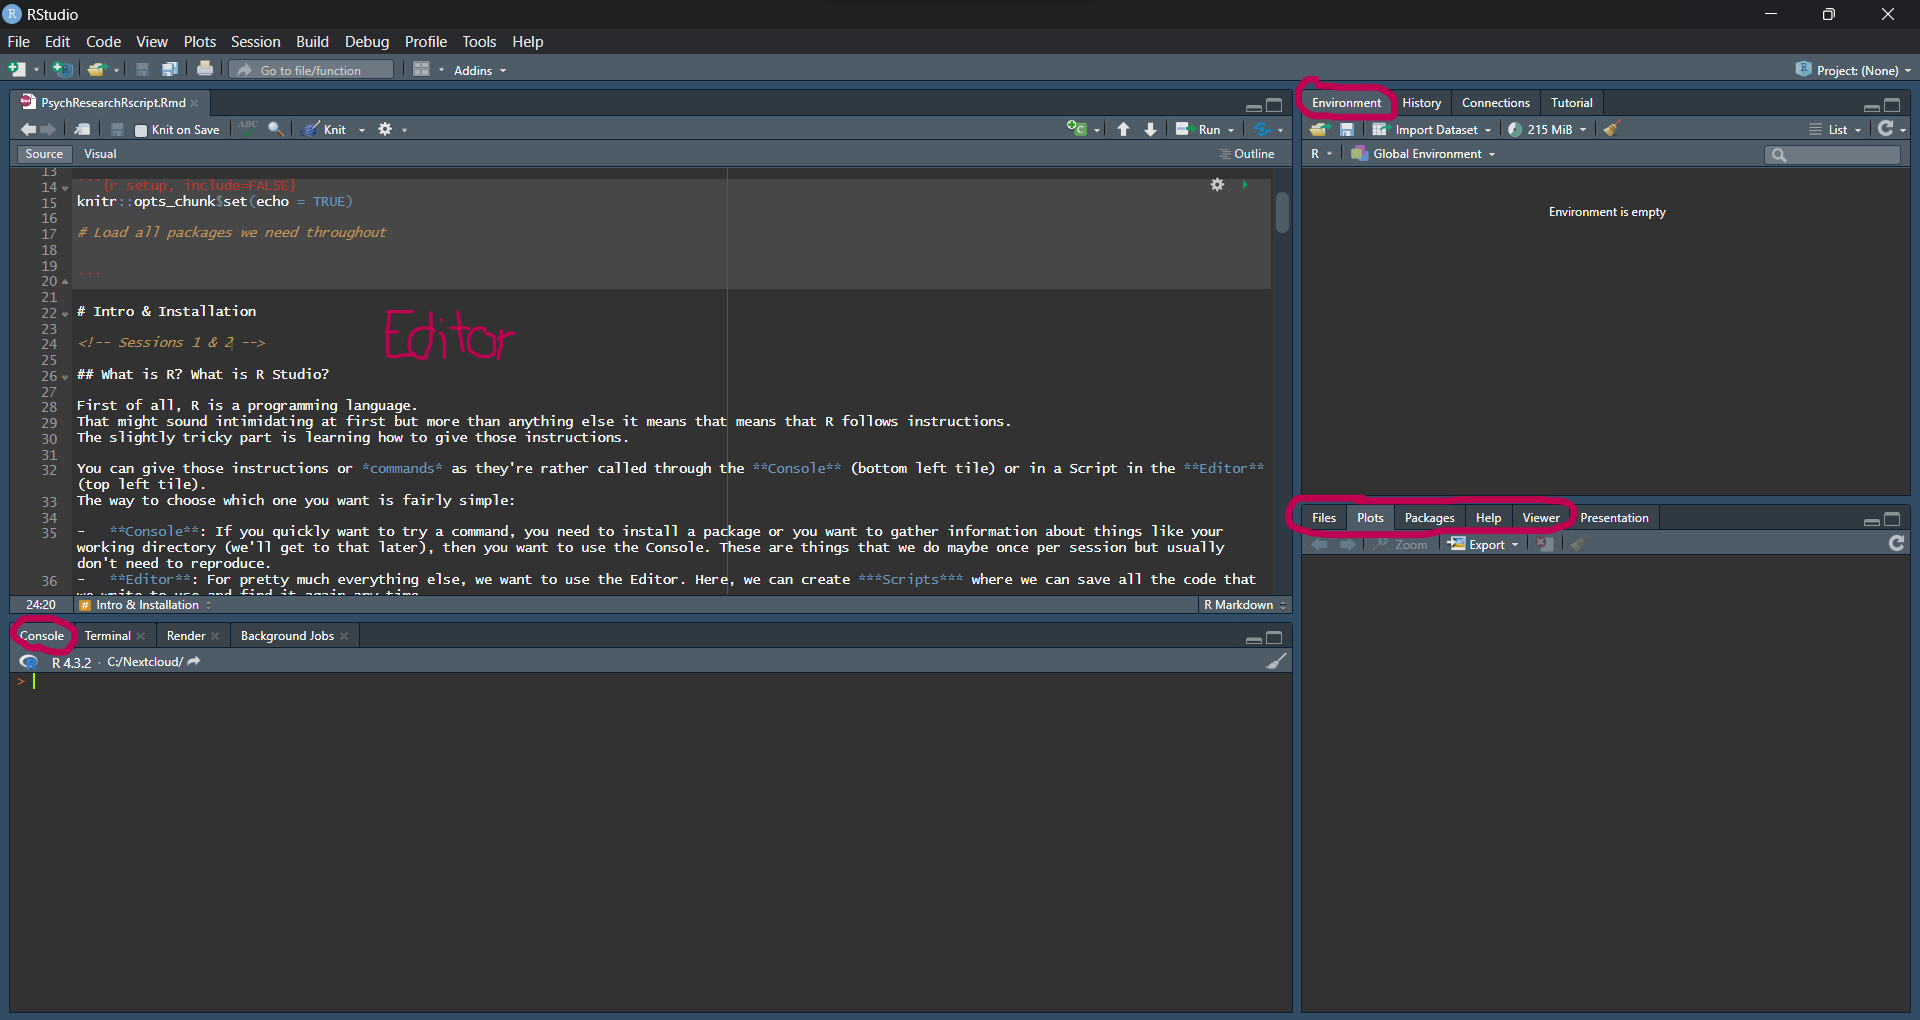
\includegraphics{./img/rstudio.png}
\caption{R Studio - typical layout}
\end{figure}

\section{Installing R and R Studio}\label{installing-r-and-r-studio}

\begin{itemize}
\tightlist
\item
  Download \& Install the newest R version 4.3.3 (2024-02-29 ucrt) at \url{https://cloud.r-project.org/}
\item
  Download and install R Studio at \url{https://posit.co/download/rstudio-desktop/}
\end{itemize}

R as a language can be used on its own.
However, it is not very modern, quite hard to use and frankly just no fun.
That's why we use R Studio as a user interface to run R.
Think of it as dipping your fingers in a pot of ink to write versus using a pen and paper - you will still write with the same ink, but the whole process is just nicer.

\subsection{Workflow}\label{workflow}

You can give instructions or \emph{commands} as they're rather called through the \textbf{Console} (bottom left tile) or in a Script in the \textbf{Editor} (top left tile).
The way to choose which one you want is fairly simple:

\begin{itemize}
\tightlist
\item
  \textbf{Console}: If you quickly want to try a command, you need to install a package or you want to gather information about things like your working directory (we'll get to that later), then you want to use the Console. These are things that we do maybe once per session but usually don't need to reproduce.
\item
  \textbf{Editor}: For pretty much everything else, we want to use the Editor. Here, we can create \textbf{\emph{Scripts}} where we can save all the code that we write to use and find again any time.
\end{itemize}

For most things - especially during the learning phase - it makes sense to write a Script in the Editor in order to be able to save and access the work.
To do so, simply click the 
\includegraphics[width=\textwidth,height=0.16667in]{./img/newfile.png} button and choose `R Script'.

Once we have a new script created, we can learn some basic things that R is capable of and save it to check out later.
Math

\begin{Shaded}
\begin{Highlighting}[]
\CommentTok{\# Basic Math}
\DecValTok{1}\SpecialCharTok{+}\DecValTok{2} 
\end{Highlighting}
\end{Shaded}

\begin{verbatim}
## [1] 3
\end{verbatim}

\begin{Shaded}
\begin{Highlighting}[]
\DecValTok{2{-}3}
\end{Highlighting}
\end{Shaded}

\begin{verbatim}
## [1] -1
\end{verbatim}

\begin{Shaded}
\begin{Highlighting}[]
\DecValTok{3}\SpecialCharTok{*}\DecValTok{4}
\end{Highlighting}
\end{Shaded}

\begin{verbatim}
## [1] 12
\end{verbatim}

\begin{Shaded}
\begin{Highlighting}[]
\DecValTok{4}\SpecialCharTok{/}\DecValTok{3}
\end{Highlighting}
\end{Shaded}

\begin{verbatim}
## [1] 1.333333
\end{verbatim}

\begin{Shaded}
\begin{Highlighting}[]
\DecValTok{5}\SpecialCharTok{\^{}}\DecValTok{2}
\end{Highlighting}
\end{Shaded}

\begin{verbatim}
## [1] 25
\end{verbatim}

\begin{Shaded}
\begin{Highlighting}[]
\CommentTok{\# Assigning Variables}
\NormalTok{a }\OtherTok{\textless{}{-}} \DecValTok{3}
\NormalTok{b }\OtherTok{\textless{}{-}} \DecValTok{4}
\NormalTok{a}\SpecialCharTok{{-}}\NormalTok{b}
\end{Highlighting}
\end{Shaded}

\begin{verbatim}
## [1] -1
\end{verbatim}

\begin{Shaded}
\begin{Highlighting}[]
\NormalTok{a}\SpecialCharTok{*}\NormalTok{b}\SpecialCharTok{+}\DecValTok{5}
\end{Highlighting}
\end{Shaded}

\begin{verbatim}
## [1] 17
\end{verbatim}

In this \texttt{code\ chunk}, R is essentially being used as a calculator to perform basic math.
While we want to make use of all the more powerful functions of R, it is important to grasp the basics and be able to use arithmetic for our purposes.
Next to the basic mathematical operators, there are many nifty mathematical functions, such as \texttt{sqrt()} - \emph{square root}, \texttt{sum()} or \texttt{pi}.

We also added \textbf{variables} containing values (here a and b hold values 3 and 4 respectively) that can be used in the calculations just like the values they contain.
As they only contain numbers, the variables a and b are called \textbf{numeric}.
We can check this property of a variable, e.g.~\texttt{a} using the function \texttt{class(a)}, which gives us ``numeric'' as output.

Usually when we fire up R, we don't just want to work with single values numeric but with \textbf{data frames} or \textbf{vectors} 
\includegraphics[width=\textwidth,height=0.20833in]{./img/vector.png} that can contain different classes of variables and several values respectively.

\begin{Shaded}
\begin{Highlighting}[]
\CommentTok{\# Vectors}
\NormalTok{c }\OtherTok{\textless{}{-}} \FunctionTok{c}\NormalTok{(}\DecValTok{6}\NormalTok{, }\DecValTok{7}\NormalTok{, }\DecValTok{8}\NormalTok{)}
\FunctionTok{class}\NormalTok{(c)}
\end{Highlighting}
\end{Shaded}

\begin{verbatim}
## [1] "numeric"
\end{verbatim}

\begin{Shaded}
\begin{Highlighting}[]
\NormalTok{d }\OtherTok{\textless{}{-}} \FunctionTok{c}\NormalTok{(}\StringTok{"sunny"}\NormalTok{, }\StringTok{"rainy"}\NormalTok{, }\StringTok{"foggy"}\NormalTok{)}
\FunctionTok{class}\NormalTok{(d)}
\end{Highlighting}
\end{Shaded}

\begin{verbatim}
## [1] "character"
\end{verbatim}

\begin{Shaded}
\begin{Highlighting}[]
\CommentTok{\# Data Frame}
\NormalTok{e }\OtherTok{\textless{}{-}} \FunctionTok{data.frame}\NormalTok{(c,d)}
\FunctionTok{class}\NormalTok{(e)}
\end{Highlighting}
\end{Shaded}

\begin{verbatim}
## [1] "data.frame"
\end{verbatim}

Notice that we did not just add all values one after the other, but followed a certain notation that begins with the function \texttt{c()}.
The c stands for ``combine'' or ``concatenate'' and tells R that all following values belong to the same variable.
There are several ways of adding variables to a data frame, but the \texttt{data.frame()} command is the simplest.

\begin{quote}
All values in a variable should have the same class.
Go ahead and try out \texttt{hm\ \textless{}-\ c(3,\ "sunny",\ 5.2)} and check the class.
What happened - did you expect that?
\end{quote}

When we have our data in a neat data frame, what we usually want to do is access either certain \textbf{rows} or \textbf{columns}.
To do so, base R uses square brackets \texttt{{[}{]}} behind the name of a data frame to indicate ``take this data, but only certain rows/columns/cells''.
Remember: The brackets understand the first input as rows and the second as columns - \emph{rows right away}.

\begin{Shaded}
\begin{Highlighting}[]
\NormalTok{e }
\end{Highlighting}
\end{Shaded}

\begin{verbatim}
##   c     d
## 1 6 sunny
## 2 7 rainy
## 3 8 foggy
\end{verbatim}

\begin{Shaded}
\begin{Highlighting}[]
\NormalTok{e[}\DecValTok{1}\NormalTok{, ]}
\end{Highlighting}
\end{Shaded}

\begin{verbatim}
##   c     d
## 1 6 sunny
\end{verbatim}

\begin{Shaded}
\begin{Highlighting}[]
\NormalTok{e[ , }\DecValTok{1}\NormalTok{]}
\end{Highlighting}
\end{Shaded}

\begin{verbatim}
## [1] 6 7 8
\end{verbatim}

\begin{Shaded}
\begin{Highlighting}[]
\NormalTok{weather }\OtherTok{\textless{}{-}}\NormalTok{ e[ , }\DecValTok{2}\NormalTok{]}
\NormalTok{weather}
\end{Highlighting}
\end{Shaded}

\begin{verbatim}
## [1] "sunny" "rainy" "foggy"
\end{verbatim}

\begin{Shaded}
\begin{Highlighting}[]
\NormalTok{e[}\DecValTok{1}\NormalTok{, }\DecValTok{1}\NormalTok{]}\SpecialCharTok{*}\NormalTok{e[}\DecValTok{2}\NormalTok{, }\DecValTok{1}\NormalTok{]}
\end{Highlighting}
\end{Shaded}

\begin{verbatim}
## [1] 42
\end{verbatim}

Our data set \texttt{e} contains three numbers in column c and different strings in column d.
We can select just the first row, or just the first column or either of the other rows and columns that we have in the data.
We can also re-assign the values, e.g.~to a new variable named ``weather'' or perform calculations on single cells in the data frame - only if they contain numerics, of course.

\begin{quote}
With square brackets we can only index rows and columns that are present in the data.
That maybe sounds obvious, but can easily lead to confusion because of error messages!
What happens when you try to index \texttt{e{[},3{]}}?
\end{quote}

While it is common practice to work with data frames and edit them according to our tasks and needs, using square brackets and base R can get a bit humdrum.
Luckily, many many people have developed many many packages that contain different functions, helping us in most tasks that we will need to tackle!

\section{Installing Packages}\label{installing-packages}

\begin{figure}
\centering
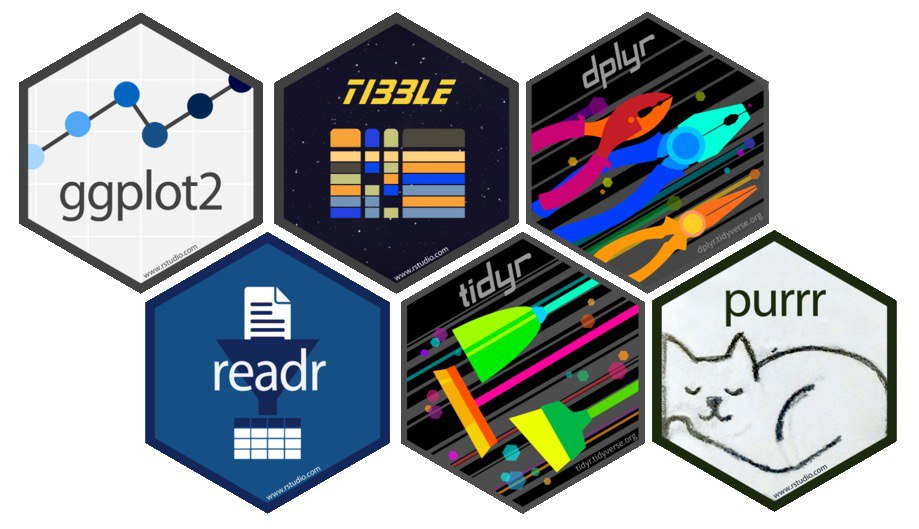
\includegraphics[width=\textwidth,height=0.625in]{./img/hexagons.png}
\caption{Hexagon Package logos}\label{id}
\end{figure}

Most packages are available on CRAN - the Comprehensive R Archive Network.
That being the case you can easily install the package you want to have with the command \texttt{install.packages("packagename")}.
It is important to note that the package name must be in quotes for the installation, while loading it into a script works without quotes using \texttt{library(packagename)}.

Packages usually serve quite specific purposes, e.g.~ones we will later get to know are \texttt{dplyr}, with which data handling is made a lot easier and more intuitive and \texttt{ggplot2}, which allows us to create beautiful, publication-ready plots and visualizations.
What is special about these two, among some others, is that they were developed by the same person (Hadley Wickham), and are made available in a sort of ``meta package'' - the \texttt{tidyverse}.
Installing and loading the \texttt{tidyverse} makes the functions from many different packages available at once.
This is quite convenient when we want to use a lot of those packages in the same session or script, but does also take a longer time to load and is sometimes not actually necessary.

To use this package of packages, please install the \texttt{tidyverse}, using \texttt{install.packages("tidyverse")} in the console and then load it into your script (or, again, directly in the console, bottom-left) with \texttt{library(tidyverse)}.
You can test whether it works by running \texttt{iris\ \%\textgreater{}\%\ pull(Sepal.Length)\ \%\textgreater{}\%\ mean()} in your console.
We will get to know the syntax in depth another time, but just so you know what's going on:
This line of code takes the data set \texttt{iris}, which is included in R by default, ``pulls'' the variable \texttt{Sepal.Length} out of the data and runs the \texttt{mean()} function on it, to calculate the average sepal length, which should be 5.8433333.

\begin{quote}
\begin{itemize}
\tightlist
\item
  R is a powerful language, R Studio is the user interface we use with it
\item
  R can be a calculator and perform basic and advanced math
\item
  We mostly work with variables and data frames
\item
  Packages make working with R easier and more fun!
\end{itemize}
\end{quote}

\begin{quote}
\begin{itemize}
\tightlist
\item
  \href{https://r-intro.tadaa-data.de/index.html}{Tadaa Data: R für Psychos (german)}
\item
  \href{https://www.kaggle.com/code/hamelg/intro-to-r-part-4-variables}{Intro to R}
\item
  \href{https://www.tidyverse.org/}{Tidyverse}
\end{itemize}
\end{quote}

\chapter{R Basics and how to read error messages}\label{r-basics-and-how-to-read-error-messages}

\begin{figure}
\centering
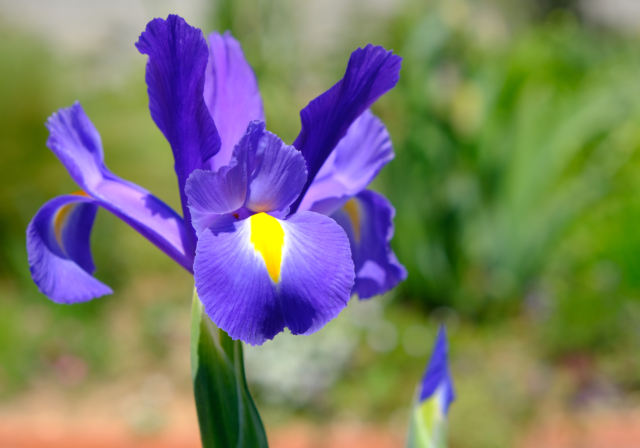
\includegraphics{img/iris.png}
\caption{Iris Flower}
\end{figure}

\section{Basics}\label{basics}

\begin{Shaded}
\begin{Highlighting}[]
\FunctionTok{library}\NormalTok{(dplyr)}
\end{Highlighting}
\end{Shaded}

R is an object-based language.
The great advantage of that is we can assign values, vectors, text, matrices or almost anything else to variables and access them more easily later.
To do that, we use the \(\leftarrow\) like so: \newline
\texttt{x\ \textless{}-\ c(1,\ 2,\ 3)}
Go ahead and try it out!
If you had too much fun assigning variables, you can remove them again from your work environment using the \texttt{rm()} command in the Console.
So, if you assign the values 1, 2 and 3 to \texttt{x}, you can type \texttt{rm(x)} into the console, hit enter and x has disappeared from your environment!

\begin{itemize}
\tightlist
\item
  Execute a line of code with \texttt{ctrl\ +\ enter} in the editor

  \begin{itemize}
  \tightlist
  \item
    In console you just need to press \texttt{enter}
  \end{itemize}
\item
  Text aka \emph{strings} need to be put in quotes so it can be recognized as such

  \begin{itemize}
  \tightlist
  \item
    \texttt{some\_text\ \textless{}-\ c("amazing",\ "wow")}
  \end{itemize}
\item
  Comments can and should be added to your code using the \texttt{\#}
\end{itemize}

\subsection{Basic Functions I}\label{basic-functions-i}

\begin{Shaded}
\begin{Highlighting}[]
\NormalTok{a }\OtherTok{\textless{}{-}} \FunctionTok{c}\NormalTok{(}\DecValTok{1}\NormalTok{, }\DecValTok{2}\NormalTok{, }\DecValTok{3}\NormalTok{, }\DecValTok{4}\NormalTok{)}
\NormalTok{b }\OtherTok{\textless{}{-}} \FunctionTok{c}\NormalTok{(}\DecValTok{5}\NormalTok{, }\DecValTok{7}\NormalTok{, }\DecValTok{9}\NormalTok{, }\DecValTok{11}\NormalTok{)}
\FunctionTok{mean}\NormalTok{(a)}
\end{Highlighting}
\end{Shaded}

\begin{verbatim}
## [1] 2.5
\end{verbatim}

\begin{Shaded}
\begin{Highlighting}[]
\FunctionTok{sd}\NormalTok{(b)}
\end{Highlighting}
\end{Shaded}

\begin{verbatim}
## [1] 2.581989
\end{verbatim}

\begin{Shaded}
\begin{Highlighting}[]
\FunctionTok{min}\NormalTok{(b)}
\end{Highlighting}
\end{Shaded}

\begin{verbatim}
## [1] 5
\end{verbatim}

\subsection{Basic Functions II}\label{basic-functions-ii}

\begin{Shaded}
\begin{Highlighting}[]
\FunctionTok{max}\NormalTok{(b)}
\end{Highlighting}
\end{Shaded}

\begin{verbatim}
## [1] 11
\end{verbatim}

\begin{Shaded}
\begin{Highlighting}[]
\NormalTok{a}\SpecialCharTok{+}\NormalTok{b}
\end{Highlighting}
\end{Shaded}

\begin{verbatim}
## [1]  6  9 12 15
\end{verbatim}

\begin{Shaded}
\begin{Highlighting}[]
\FunctionTok{sum}\NormalTok{(b)}
\end{Highlighting}
\end{Shaded}

\begin{verbatim}
## [1] 32
\end{verbatim}

\begin{Shaded}
\begin{Highlighting}[]
\FunctionTok{length}\NormalTok{(a)}
\end{Highlighting}
\end{Shaded}

\begin{verbatim}
## [1] 4
\end{verbatim}

\subsection{Basic Functions III}\label{basic-functions-iii}

\begin{Shaded}
\begin{Highlighting}[]
\NormalTok{c }\OtherTok{\textless{}{-}} \DecValTok{3}\SpecialCharTok{:}\DecValTok{9}
\NormalTok{c }\CommentTok{\# look at the variable}
\end{Highlighting}
\end{Shaded}

\begin{verbatim}
## [1] 3 4 5 6 7 8 9
\end{verbatim}

\begin{Shaded}
\begin{Highlighting}[]
\FunctionTok{range}\NormalTok{(c)}
\end{Highlighting}
\end{Shaded}

\begin{verbatim}
## [1] 3 9
\end{verbatim}

\begin{Shaded}
\begin{Highlighting}[]
\NormalTok{d }\OtherTok{\textless{}{-}} \FunctionTok{c}\NormalTok{(}\DecValTok{10}\SpecialCharTok{:}\DecValTok{15}\NormalTok{, }\DecValTok{20}\SpecialCharTok{:}\DecValTok{25}\NormalTok{)}
\end{Highlighting}
\end{Shaded}

\section{Basic Functions IV}\label{basic-functions-iv}

\begin{Shaded}
\begin{Highlighting}[]
\NormalTok{d }\CommentTok{\# look at the variable}
\end{Highlighting}
\end{Shaded}

\begin{verbatim}
##  [1] 10 11 12 13 14 15 20 21 22 23 24 25
\end{verbatim}

\begin{Shaded}
\begin{Highlighting}[]
\NormalTok{d[}\DecValTok{1}\NormalTok{] }\CommentTok{\# index}
\end{Highlighting}
\end{Shaded}

\begin{verbatim}
## [1] 10
\end{verbatim}

\begin{Shaded}
\begin{Highlighting}[]
\NormalTok{d[d}\SpecialCharTok{==}\DecValTok{10}\NormalTok{]}
\end{Highlighting}
\end{Shaded}

\begin{verbatim}
## [1] 10
\end{verbatim}

\begin{Shaded}
\begin{Highlighting}[]
\FunctionTok{which}\NormalTok{(d}\SpecialCharTok{==}\DecValTok{12}\NormalTok{)}
\end{Highlighting}
\end{Shaded}

\begin{verbatim}
## [1] 3
\end{verbatim}

\section{Exercise}\label{exercise}

Create a vector x with the numbers from 50 to 100 and 150 to 200.

Find its mean, standard deviation and its range.

What is the 77th number of vector x?

\subsection{Solution}\label{solution}

\begin{itemize}
\tightlist
\item
  \texttt{x\ \textless{}-\ c(50:100,\ 150:200)}\strut \\
\item
  \texttt{mean(x),\ sd(x),\ range(x)\ \%\textgreater{}\%\ round(2)}: \newline 125, 52.38, 50, 200

  \begin{itemize}
  \tightlist
  \item
    \texttt{\%\textgreater{}\%\ round(2)} takes the numbers and rounds them up to two decimal points
  \end{itemize}
\item
  \texttt{x{[}77{]}}: 175
\end{itemize}

\subsection{\texorpdfstring{Brainteaser }{Brainteaser }}\label{brainteaser}

We define two variables in the following way:

\begin{Shaded}
\begin{Highlighting}[]
\NormalTok{e }\OtherTok{\textless{}{-}} \DecValTok{1}\SpecialCharTok{:}\DecValTok{5}
\NormalTok{f }\OtherTok{\textless{}{-}} \DecValTok{2}\SpecialCharTok{:}\DecValTok{5}
\end{Highlighting}
\end{Shaded}

Let's say we want to access the number 5 in both variables.
How come \texttt{e{[}5{]}} works but \texttt{f{[}5{]}} does not?

\section{Logic}\label{logic}

\begin{itemize}
\tightlist
\item
  next to numeric and string variables: \emph{boolean}

  \begin{itemize}
  \tightlist
  \item
    either hold the value \textbf{TRUE} or \textbf{FALSE} (also 1 or 0 respectively)
  \end{itemize}
\item
  useful for filtering data

  \begin{itemize}
  \tightlist
  \item
    also for conditional operations and recoding
  \end{itemize}
\end{itemize}

\subsection{Logical Examples I}\label{logical-examples-i}

\begin{Shaded}
\begin{Highlighting}[]
\NormalTok{a }\OtherTok{\textless{}{-}} \DecValTok{4}\NormalTok{; b }\OtherTok{\textless{}{-}} \DecValTok{5}
\NormalTok{a }\SpecialCharTok{\textless{}}\NormalTok{ b }\CommentTok{\# smaller than}
\end{Highlighting}
\end{Shaded}

\begin{verbatim}
## [1] TRUE
\end{verbatim}

\begin{Shaded}
\begin{Highlighting}[]
\NormalTok{a }\SpecialCharTok{\textless{}=} \DecValTok{4} \CommentTok{\# smaller/ equal}
\end{Highlighting}
\end{Shaded}

\begin{verbatim}
## [1] TRUE
\end{verbatim}

\begin{Shaded}
\begin{Highlighting}[]
\NormalTok{a }\SpecialCharTok{\textgreater{}}\NormalTok{ b }\CommentTok{\# greater than}
\end{Highlighting}
\end{Shaded}

\begin{verbatim}
## [1] FALSE
\end{verbatim}

\begin{Shaded}
\begin{Highlighting}[]
\NormalTok{a }\SpecialCharTok{\textgreater{}=} \DecValTok{3} \CommentTok{\# greater/ equal}
\end{Highlighting}
\end{Shaded}

\begin{verbatim}
## [1] TRUE
\end{verbatim}

\subsection{Logical Examples II}\label{logical-examples-ii}

\begin{Shaded}
\begin{Highlighting}[]
\NormalTok{a }\SpecialCharTok{==}\NormalTok{ b }\CommentTok{\# double equal sign!!}
\end{Highlighting}
\end{Shaded}

\begin{verbatim}
## [1] FALSE
\end{verbatim}

\begin{Shaded}
\begin{Highlighting}[]
\NormalTok{a }\SpecialCharTok{!=}\NormalTok{ b}
\end{Highlighting}
\end{Shaded}

\begin{verbatim}
## [1] TRUE
\end{verbatim}

\begin{Shaded}
\begin{Highlighting}[]
\NormalTok{c }\OtherTok{\textless{}{-}} \ConstantTok{TRUE}
\NormalTok{c}
\end{Highlighting}
\end{Shaded}

\begin{verbatim}
## [1] TRUE
\end{verbatim}

\begin{Shaded}
\begin{Highlighting}[]
\SpecialCharTok{!}\NormalTok{c}
\end{Highlighting}
\end{Shaded}

\begin{verbatim}
## [1] FALSE
\end{verbatim}

\subsection{Putting it all together\ldots{}}\label{putting-it-all-together}

\subsubsection{Exercise}\label{exercise-1}

\textbf{We want to find out whether the average Petal Length and Sepal Length of iris flowers are different from each other.}

Use what you know to ``ask R'' if those values are unequal!

Hint: You will need logic, the mean()-function and square brackets. Use \textbf{names(iris)} to find all variable names in that data set.

\subsection{Solution}\label{solution-1}

\begin{itemize}
\tightlist
\item
  Square bracket indexing with the variable name in quotes \newline
  \texttt{iris{[}\ ,\ "Sepal.Length"{]}}\\
  \texttt{iris{[}\ ,\ "Petal.Length"{]}}
\item
  now we add the mean function around both like this:
  \texttt{mean(iris{[}\ ,\ "Sepal.Length"{]})}\\
  \texttt{mean(iris{[}\ ,\ "Sepal.Length"{]})}
\item
  Finally we compare the two with the != operator:
  \texttt{mean(iris{[}\ ,\ "Sepal.Length"{]})\ !=}
  \texttt{mean(iris{[}\ ,\ "Petal.Length"{]})}\\
  TRUE
\end{itemize}

\section{Reading Error Messages}\label{reading-error-messages}

Even the most advanced R coder will encounter the occasional error message.
While they are quite helpful and usually lead to being able to solve problems, it can be challenging to learn how to properly read the message in order to actually understand what the problem is.
Therefore, we will look at some of the most common wordings to decipher what R needs so it can understand what we want to do.

Think of error messages not as discouraging faults of your program but rather as invites to help you help R understand what you are trying to achieve.

\subsubsection*{\texorpdfstring{\emph{Error: unexpected `X' in ``Y''}}{Error: unexpected `X' in ``Y''}}\label{error-unexpected-x-in-y}
\addcontentsline{toc}{subsubsection}{\emph{Error: unexpected `X' in ``Y''}}

This message is fairly straightforward:
R expected a certain kind of symbol at the place where we put `X' and is now confused because our input did not match the expectation.

For most Europeans, for example, the most commonly used decimal separator will be a comma.
Since R is an american-built language, however, it expects decimals to be separated with a decimal point while commas indicate separate inputs to a function.
Therefore, when we accidentally input a decimal as `3,141', we will receive the error message \emph{Error: unexpected `,' in ``3,''} because R expected the input to be something like `3.141'.

\textbf{Fix: Replace the `x' in ``Y'' with something that R can understand.} Or alternatively: Make sure that we meant the input like that.

\subsubsection*{\texorpdfstring{\emph{Error: object `A' not found}}{Error: object `A' not found}}\label{error-object-a-not-found}
\addcontentsline{toc}{subsubsection}{\emph{Error: object `A' not found}}

This, too, is pretty understandable message:
The object that you are trying to access and use cannot be found by R.
The most common cause for this error message is probably simply that you misspelled the object name somewhere.
R is case-sensitive, so maybe object \emph{A} was defined as object \emph{a}?
Maybe the object \emph{vector} is spelled \emph{vcteor} in your function?

Moreover, sometimes our thoughts are two steps ahead of our code.
When figuring out how to get a program to work, sometimes we presume that a variable exists just because we need it and forget to define the variable up front.
The same goes if we try to access a variable in a data frame that was maybe defined in a different data frame or as its own vector - it simply cannot be found because we are having R look in the wrong place.

\textbf{Fix: Make sure the object name is spelled correctly and was defined prior to using it in a function, calculation or elsewhere.}

This error message also often appears with ``function xyz not found''.
In this case, we probably forgot to load the package first, which contains that function.
Thus, the fix will likely be to figure out which package contains the function we are trying to use and load it with the \texttt{library()} command.

\begin{itemize}
\item
  \begin{figure}
  \centering
  \includegraphics[width=\textwidth,height=2.08333in]{./img/nerfect.webp}
  \caption{Pobody's Nerfect}\label{id}
  \end{figure}
\end{itemize}

\subsection{\texorpdfstring{\emph{Error}: R does nothing after running a command}{Error: R does nothing after running a command}}\label{error-r-does-nothing-after-running-a-command}

\begin{itemize}
\item
  This is not an error message but still very common, especially at the beginning
\item
  Usually, there is a \texttt{\textgreater{}} symbol at the beginning of our console input line

  \begin{itemize}
  \tightlist
  \item
    If R is ``unfinished'' with a command, you see \texttt{+} instead
  \end{itemize}
\item
  This happens when R can`t work with the command because there is something missing

  \begin{itemize}
  \tightlist
  \item
    In most cases, this will be closing parentheses
  \end{itemize}
\item
  \(\rightarrow\) \textbf{Fix: Click in your console and use the \texttt{Esc} button to cancel the command. Then, look at the code you were trying to run and see if there is some closing statement such as \texttt{)} missing and try again.}
\item
  We have not talked about the \%\textgreater\%-pipe in depth, but you will hopefully start to love this tool and use it a lot
\item
  If we end a command with a \%\textgreater\% R will show the same behavior of not executing the code

  \begin{itemize}
  \tightlist
  \item
    \(\rightarrow\) R expects something else after the pipe, so when there's nothing, R is confused \includegraphics[width=\textwidth,height=1.04167in]{./img/waitforit.gif}
  \end{itemize}
\item
  When you need help figuring out how a function works, there are several ways to get it. Try typing \textbf{?magrittr::`\%\textgreater\%`} into your console and hit enter!
\end{itemize}

\section{Exercise}\label{exercise-2}

Below is some code that has a few problems.

Try to identify them and how they might be fixed. Feel free to test them out if you are not sure!

\texttt{Library(greatpackage)}

Solution

\begin{itemize}
\tightlist
\item
  \texttt{library} should not be capitalized
\item
  ``greatpackage'' does not exist and can thus not be loaded
\end{itemize}

\texttt{mean(coolvariable)}

Solution

coolvariable was not defined previously

\texttt{a\ \textless{}-\ c(1,\ 3,\ 6,\ 7}

Solution

the command is not finished, it needs a closing parentheses

\texttt{b\ \textless{}-\ c(2,\ 4;\ 6,\ 8)}

Solution

we need all commas to separate numbers in a vector, not a semicolon

\section{Wrap-Up \& Further Resources}\label{wrap-up-further-resources}

Functions work with input inside round brackets, e.g.~c(1, 2, 3)

a point \textbf{.} is a decimal separator in numbers; a comma \textbf{,} seperates input in functions

Logical operators compare data, e.g.~7 \textgreater{} 6 would output TRUE

\texttt{\#} allows comments in the code

Errors should be invitations to make your code more understandable for R

\(\rightarrow\) the better we understand the problem, the better we can fix it!

\href{https://stackoverflow.com/}{StackOverflow}

\href{https://katalog.uni-konstanz.de/libero/WebOpac.cls?VERSION=2&ACTION=DISPLAY&RSN=2222774&DATA=KON&TOKEN=nGIfSiZsIA5826&Z=1&SET=1}{Discovering Statistics Using R} Book by Andy Field, available from KIM

\chapter{Best Practice}\label{best-practice}

\section{What is Best Practice?}\label{what-is-best-practice}

\begin{itemize}
\tightlist
\item
  ``Many roads lead to Rome'': You can achieve most things in many different ways
\item
  \emph{Best Practice} refers to the best/ easiest/ clearest way of working with R
\end{itemize}

\subsection{Overview}\label{overview}

\begin{itemize}
\tightlist
\item
  Naming Variables
\item
  Creating data meaningfully
\item
  Working Directories
\item
  R Projects
\item
  Make R your own: 
\includegraphics[width=\textwidth,height=0.41667in]{./img/appearance.png}
\end{itemize}

\section{Naming Conventions}\label{naming-conventions}

R is a so-called \emph{object-oriented} language.
What that means for us is mostly that all our data exist as ``objects'' as far is R is concerned.
Just like in real life, we can \emph{do} stuff with those objects now, which is called using a \emph{function} or \emph{command}.
Which brings me to the importance of proper names for all your variables, data sets, functions\ldots{}
Everything.

If we go to the market and I tell you to get me an apple, you will probably be confused if there are many types of apples, maybe different colors, maybe different breeds.
Basically, if I don't specify which apple I want, you are not able to pick out the right one.
The same is true for R: If you try to call a function but fail to specify what object to use the function on, R is confused and throws you an error.

Now, this may seem pretty obvious but it is a pretty common source of errors, especially during the ``steep phase'' of the learning curve.
In R, \texttt{abc} is a different object than \texttt{ABC}, which is different from \texttt{a\_b\_c}, which is different from \texttt{A.B.C}. All of these variants are possible ways of naming your objects in R.
However, it makes everyone's life significantly easier to stick to some naming-guidelines.

\begin{itemize}
\tightlist
\item
  Preferably use \textbf{lower-case} variable names, e.g.~\texttt{gender} instead of \texttt{Gender} or \texttt{GENDER}.
\item
  Preferably use an \textbf{underscore} to differentiate between different words in your object names if necessary, e.g.~\texttt{music\_preference}.
\item
  \textbf{Avoid using numbers} in your names because likely either you or R will get confused with this at some point, e.g.~\texttt{raw\_data} instead of \texttt{data1}\footnote{Additionally, the 1 (one) and the l (lower-case L) can look very similar, which makes thing just even worse when trying to figure out an error.}.
\item
  Use \textbf{abbreviations} where useful, e.g.~\texttt{rt} instead of \texttt{reaction\_times}.
\item
  Use \textbf{names that will still make sense} to you in the future, i.e.~avoid names like \texttt{asdf\_data} or \texttt{blibblobfundata}. The best case scenario would be that your variable names also makes sense to other people if they try to understand your code!
\end{itemize}

I will admit that some of these pieces of advice are more opinionated personal experience than objective facts.
The more you work with variables and maybe also code from other people, you may form your own opinions on what the best naming conventions are for you.
I strongly suggest finding a way that works for you and sticking with it.
As I described above, I personally will try to stick to \emph{lower\_snake\_case} to name my variables because it is usually very clear, easy to read by humans and computers and would also be usable in any other programming language.

Another thing that can take some time to get used to is avoiding white spaces in file names and any other names, for that matter.
R has problems finding files with names such as ``My file with a really specific name.bib'', which can easily be avoided by sticking to snake\_case: ``My\_file\_with\_a\_really\_specific\_name.bib''.
The same goes for variables: In my first class, we discovered that it is possible in R to set a variable name with a space.
Just because it's possible does not mean anybody should do it. Ever.

You can try it out: Enter \texttt{"hi\ there"\ \textless{}-\ 5} in your console to assign the value 5 to a variable named \texttt{hi\ there}.
You will see it appear in your working environment, but accessing the variable is virtually impossible.
If you just type \texttt{hi\ there} in the console and hit Enter, R will give you an error à la \emph{``unexpected symbol''}.
But if you type \texttt{"hi\ there"}, it will echo the text back to you.

\begin{figure}
\centering
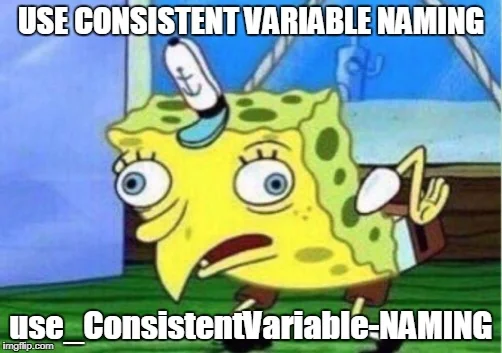
\includegraphics[width=\textwidth,height=4.16667in]{./img/varname.webp}
\caption{Naming Conventions}\label{id}
\end{figure}

\url{https://www.reddit.com/r/ProgrammerHumor/comments/6stwag/can_you_stick_to_any_naming_convention/}

\subsection{Exercise: Name Examples}\label{exercise-name-examples}

\begin{itemize}
\tightlist
\item
  \texttt{great\ variable}

  \begin{itemize}
  \tightlist
  \item
    Spaces can technically work but are a hassle to access
  \end{itemize}
\item
  \texttt{Areallysuperinsanelyverylongvariablename}

  \begin{itemize}
  \tightlist
  \item
    Variables are supposed to \emph{reduce} workload
  \end{itemize}
\item
  \texttt{Howaboutthis\$}

  \begin{itemize}
  \tightlist
  \item
    Special characters should be avoided
  \end{itemize}
\item
  \texttt{age\_grouped}

  \begin{itemize}
  \tightlist
  \item
  \end{itemize}
\item
  \texttt{GenderRecoded}

  \begin{itemize}
  \tightlist
  \item
  \end{itemize}
\item
  \texttt{aMAZING¯vARIABLE¯nAME}

  \begin{itemize}
  \tightlist
  \item
    Please just no.
  \end{itemize}
\end{itemize}

\section{Scenario: Creating Data meaningfully}\label{scenario-creating-data-meaningfully}

Imagine we are going to measure some test scores at a school that are supposed to reflect the kids' IQ (mean 100, sd 15).
In order to prepare for data analysis, we want to simulate what the data might look like beforehand.

We are going to measure their age and IQ score and we will be assessing class 7a and 7b.

\subsection{Exercise: Creating Data meaningfully}\label{exercise-creating-data-meaningfully}

Create \textbf{two data frames} - one for each class.
They should each contain \textbf{n = 20 entries} (for 20 kids) and \textbf{2 variables i.e.~age and iq score}.
We assume \textbf{age is a random number from 12 to 15} and \textbf{iq follows normal distribution with mean = 100, sd = 15}.

Afterwards, add a variable to code the \textbf{class} to each data frame and add them together \textbf{underneath each other}.
Use the functions on the board and look in the R help if you need more input on how to use them.

\subsection{Solution}\label{solution-2}

\begin{Shaded}
\begin{Highlighting}[]
\CommentTok{\# Create the dataframes}
\NormalTok{scores7a }\OtherTok{\textless{}{-}} \FunctionTok{data.frame}\NormalTok{(}\AttributeTok{age =} \FunctionTok{sample}\NormalTok{(}\AttributeTok{x =} \DecValTok{12}\SpecialCharTok{:}\DecValTok{15}\NormalTok{, }\AttributeTok{size =} \DecValTok{20}\NormalTok{, }\AttributeTok{replace =}\NormalTok{ T),}
                       \AttributeTok{iq =} \FunctionTok{rnorm}\NormalTok{(}\AttributeTok{n =} \DecValTok{20}\NormalTok{, }\AttributeTok{mean =} \DecValTok{100}\NormalTok{, }\AttributeTok{sd =} \DecValTok{15}\NormalTok{))}

\NormalTok{scores7b }\OtherTok{\textless{}{-}} \FunctionTok{data.frame}\NormalTok{(}\AttributeTok{age =} \FunctionTok{sample}\NormalTok{(}\AttributeTok{x =} \DecValTok{12}\SpecialCharTok{:}\DecValTok{15}\NormalTok{, }\AttributeTok{size =} \DecValTok{20}\NormalTok{, }\AttributeTok{replace =}\NormalTok{ T),}
                       \AttributeTok{iq =} \FunctionTok{rnorm}\NormalTok{(}\AttributeTok{n =} \DecValTok{20}\NormalTok{, }\AttributeTok{mean =} \DecValTok{100}\NormalTok{, }\AttributeTok{sd =} \DecValTok{15}\NormalTok{))}
\CommentTok{\# Notice anything about the code?}

\FunctionTok{str}\NormalTok{(scores7a); }\FunctionTok{str}\NormalTok{(scores7b)}
\end{Highlighting}
\end{Shaded}

\begin{verbatim}
## 'data.frame':    20 obs. of  2 variables:
##  $ age: int  15 12 12 12 15 12 13 14 12 15 ...
##  $ iq : num  101.1 98.9 107.2 90.1 107.8 ...
\end{verbatim}

\begin{verbatim}
## 'data.frame':    20 obs. of  2 variables:
##  $ age: int  13 12 12 14 15 13 12 13 12 12 ...
##  $ iq : num  98.2 101.6 120.2 99.3 74.2 ...
\end{verbatim}

\begin{Shaded}
\begin{Highlighting}[]
\CommentTok{\# Add information about the class}
\NormalTok{scores7a}\SpecialCharTok{$}\NormalTok{class }\OtherTok{\textless{}{-}} \StringTok{"7a"}
\NormalTok{scores7b}\SpecialCharTok{$}\NormalTok{class }\OtherTok{\textless{}{-}} \StringTok{"7b"}

\CommentTok{\# create big dataframe}
\NormalTok{allscores }\OtherTok{\textless{}{-}} \FunctionTok{rbind}\NormalTok{(scores7a, scores7b)}

\CommentTok{\# Check the overall data frame for plausibility}
\FunctionTok{str}\NormalTok{(allscores)}
\end{Highlighting}
\end{Shaded}

\begin{verbatim}
## 'data.frame':    40 obs. of  3 variables:
##  $ age  : int  15 12 12 12 15 12 13 14 12 15 ...
##  $ iq   : num  101.1 98.9 107.2 90.1 107.8 ...
##  $ class: chr  "7a" "7a" "7a" "7a" ...
\end{verbatim}

\begin{Shaded}
\begin{Highlighting}[]
\FunctionTok{table}\NormalTok{(allscores}\SpecialCharTok{$}\NormalTok{class)}
\end{Highlighting}
\end{Shaded}

\begin{verbatim}
## 
## 7a 7b 
## 20 20
\end{verbatim}

\section{Working Directories}\label{working-directories}

\begin{itemize}
\tightlist
\item
  A working directory corresponds to the folder on your computer that you are \textbf{working in}

  \begin{itemize}
  \tightlist
  \item
    If you save a script, it will be saved there
  \end{itemize}
\item
  We usually work with data from other sources or different files

  \begin{itemize}
  \tightlist
  \item
    e.g.~WEXTOR data or bibfiles for bibliography
  \end{itemize}
\item
  Check your working directory: \texttt{getwd()}
\item
  Manually set your working directory: \texttt{setwd()}

  \begin{itemize}
  \tightlist
  \item
    Any file you want to use, e.g.~containing data will be searched in that folder
  \end{itemize}
\end{itemize}

\subsection{Try it out!}\label{try-it-out}

Execute the getwd() command in the console.
Which folder is R working in, is it the one you expected?

\subsection{Cautionary Tale}\label{cautionary-tale}

\begin{itemize}
\tightlist
\item
  The file path in \texttt{getwd()} will always be \emph{absolute} \(\rightarrow\) full file path from \emph{your} computer

  \begin{itemize}
  \tightlist
  \item
    Sharing is difficult
  \item
    Working with that script on your other computer is difficult
  \item
    Nobody else can (easily) reproduce your code
  \end{itemize}
\item
  It is easy to forget which folder you're working on and which one you want to be working on

  \begin{itemize}
  \tightlist
  \item
    So R won't find files you're looking for and throw errors
  \end{itemize}
\end{itemize}

\section{R Projects}\label{r-projects}

\begin{itemize}
\tightlist
\item
  Solution: Create an R Project for your project!

  \begin{itemize}
  \tightlist
  \item
    Automatically sets your working directory to the folder you put the project in
  \item
    Makes sharing your project easy
  \item
    Saves you time and frustration, trust me
  \end{itemize}
\end{itemize}

\subsection{Let's try that out!}\label{lets-try-that-out}

Under \texttt{File} \(\rightarrow\) \texttt{New\ project...}

\subsection{Homework: Put it to the test}\label{homework-put-it-to-the-test}

\begin{enumerate}
\def\labelenumi{\arabic{enumi}.}
\tightlist
\item
  Create a subfolder called ``data'' in your R project.
\item
  Download the file ``mindfulness\_data.Rds'' from ILIAS and save it in that folder.
\item
  Now try to load it into your script and check whether it worked by typing:
\end{enumerate}

\begin{Shaded}
\begin{Highlighting}[]
\NormalTok{mindful }\OtherTok{\textless{}{-}} \FunctionTok{readRDS}\NormalTok{(}\StringTok{"./data/mindfulness\_data.Rds"}\NormalTok{) }\CommentTok{\# relative filepath}
\FunctionTok{str}\NormalTok{(mindful)}
\end{Highlighting}
\end{Shaded}

\begin{verbatim}
## tibble [601 x 6] (S3: tbl_df/tbl/data.frame)
##  $ observing : num [1:601] 3.9 3.8 5 3.5 3.7 3.2 3.9 3 3.6 3.1 ...
##  $ describing: num [1:601] 3 2.9 3.5 3 3.3 3.1 2.9 2.9 3 3 ...
##  $ accepting : num [1:601] 3.7 4.6 1.7 3.9 4 3.3 1.7 3.1 2.2 4.1 ...
##  $ acting    : num [1:601] 2.7 3.8 2.8 3 3.3 4 2.4 3.4 3 3 ...
##  $ age       : num [1:601] 38 26 53 56 18 34 70 24 31 43 ...
##  $ gender    : Factor w/ 3 levels "male","female",..: 2 1 2 1 1 1 2 2 1 1 ...
\end{verbatim}

\section{Make R your own: Appearance}\label{make-r-your-own-appearance}

\begin{itemize}
\tightlist
\item
  There are many different ``themes'' for R Studio

  \begin{itemize}
  \tightlist
  \item
    Control not only what the interface looks like but also how code is displayed
  \end{itemize}
\item
  Under \texttt{Tools} \(\rightarrow\) \texttt{Global\ Options} \(\rightarrow\) \texttt{Appearance}
\end{itemize}

\subsection{Why?}\label{why}

\begin{itemize}
\tightlist
\item
  Honestly? Because It's fun.
\item
  If a program is no fun, you won't like using it

  \begin{itemize}
  \tightlist
  \item
    And if you don't like using it, you won't get the practice you need!
  \end{itemize}
\end{itemize}

\section{Not-so-secret keyboard shortcuts to make your life easier}\label{not-so-secret-keyboard-shortcuts-to-make-your-life-easier}

\begin{longtable}[]{@{}ll@{}}
\toprule\noalign{}
Function & Shortcut PC / Mac \\
\midrule\noalign{}
\endhead
\bottomrule\noalign{}
\endlastfoot
Run current line & Ctrl + Enter / Cmd + Return \\
Add \textless- & Alt + - / Option + - \\
Add \%\textgreater\% & Ctrl + Shift + M / Cmd + Shift + M \\
Show help & F1 \\
Options for auto-fill & Tab \\
Create New Script & Ctrl + Shift + N / Cmd + Shift + N \\
Comment out line & Ctrl + Shift + C / Cmd + Shift + C \\
Save your script & Ctrl + S / Cmd + S \\
\end{longtable}

\section{Wrap-Up \& Further Resources}\label{wrap-up-further-resources-1}

\begin{quote}
Stick to naming conventions for R objects and related files

Make sure your working directory is correct

Use R projects to organize your scripts easily

Make R fun and appealing to use FOR YOU!
\end{quote}

\href{https://thedavidchen.github.io/post/rstudio-why-use-projects/}{R Projects: A quick overview}

\href{https://bookdown.org/daniel_dauber_io/r4np_book/starting-your-r-projects.html}{Starting your R projects}

\href{https://martinctc.github.io/blog/rstudio-projects-and-working-directories-a-beginner's-guide/}{RStudio Projects and Directories} (rather thorough)

\chapter{\texorpdfstring{Into the \texttt{tidyverse}: Data munging with \texttt{dplyr}}{Into the tidyverse: Data munging with dplyr}}\label{into-the-tidyverse-data-munging-with-dplyr}

\section{\texorpdfstring{Working with packages }{Working with packages }}\label{working-with-packages}

\begin{itemize}
\tightlist
\item
  install packages with \texttt{install.packages()}

  \begin{itemize}
  \tightlist
  \item
    Only once in the console!
  \end{itemize}
\item
  load packages with \texttt{library()}

  \begin{itemize}
  \tightlist
  \item
    Every time you load a script or start a new session
  \item
    Usually in the script, but also in the console
  \end{itemize}
\item
  Specific function from a package: \texttt{package::function()}

  \begin{itemize}
  \tightlist
  \item
    Use if you just need that one function once and don't want load the entire package
  \item
    Or to explicitly show the according package
  \item
    Or the function name is also in other packages (e.g.~``filter'' is usually \texttt{dplyr::filter}, but sometimes \texttt{stats::filter})
  \end{itemize}
\end{itemize}

\subsection{Incomplete List of Useful Packages}\label{incomplete-list-of-useful-packages}

\subsubsection{For Reference}\label{for-reference}

\begin{longtable}[]{@{}ll@{}}
\toprule\noalign{}
Package Name & General Purpose \\
\midrule\noalign{}
\endhead
\bottomrule\noalign{}
\endlastfoot
psych & Advanced statistical testing / modeling e.g.~factor analysis \\
tibble & Alternative for creating data frames \\
tidyr & Clean up daata \& simple reshaping \\
dropR & Dropout analysis (by experimental condition) \\
foreign & Handling data from SPSS \\
corrplot & Create correlation plots/ matrices \\
\end{longtable}

\subsection{The tidyverse}\label{the-tidyverse}

``The tidyverse is an opinionated \textbf{collection of R packages designed for data science}. All packages share an underlying design philosophy, grammar, and data structures.'' \url{tidyverse.org}

\begin{itemize}
\tightlist
\item
  The features are very intuitive and clear
\item
  It is easy and makes sense to combine several features of those packages
\item
  We will focus on aspects of \emph{literal everyday use}:

  \begin{itemize}
  \tightlist
  \item
    Clean up data aka. data wrangling \(\rightarrow\) { \texttt{dplyr} }
  \item
    Visualize data for overview or reporting \(\rightarrow\) \texttt{ggplot2}
  \end{itemize}
\end{itemize}

\section{\texorpdfstring{What is \texttt{dplyr}?}{What is dplyr?}}\label{what-is-dplyr}

\begin{figure}
\centering

\includegraphics[width=\textwidth,height=0.83333in]{./img/dplyr.png}
\caption{dplyr logo}
\end{figure}

\begin{itemize}
\item
  Probably the best and most important package in R
\item
  Powerful tool for editing data in data frames
\item
  Great way to keep your workflow clear and reproducible
\item
  Very intuitively named functions
\item
  \texttt{install.packages("dplyr")} \(\rightarrow\) \texttt{library(dplyr)}
\end{itemize}

\subsection{\texorpdfstring{Most important \texttt{dplyr} functions}{Most important dplyr functions}}\label{most-important-dplyr-functions}

\begin{itemize}
\item
  \texttt{select()}: select certain columns by name
\item
  \texttt{filter()}: filter values from a column/variable
\item
  \texttt{rename()}: rename a variable
\item
  \texttt{mutate()}: change values of a column (new or existing)
\item
  \texttt{\%\textgreater{}\%}: ``pipe'' brings data from previous operation to the next (Shortcut: Strg + Shift + M)
\item
  Cheatsheet: \url{https://github.com/rstudio/cheatsheets/blob/main/data-transformation.pdf}
\end{itemize}

\section{Intro to the exercise}\label{intro-to-the-exercise}

\begin{figure}
\centering
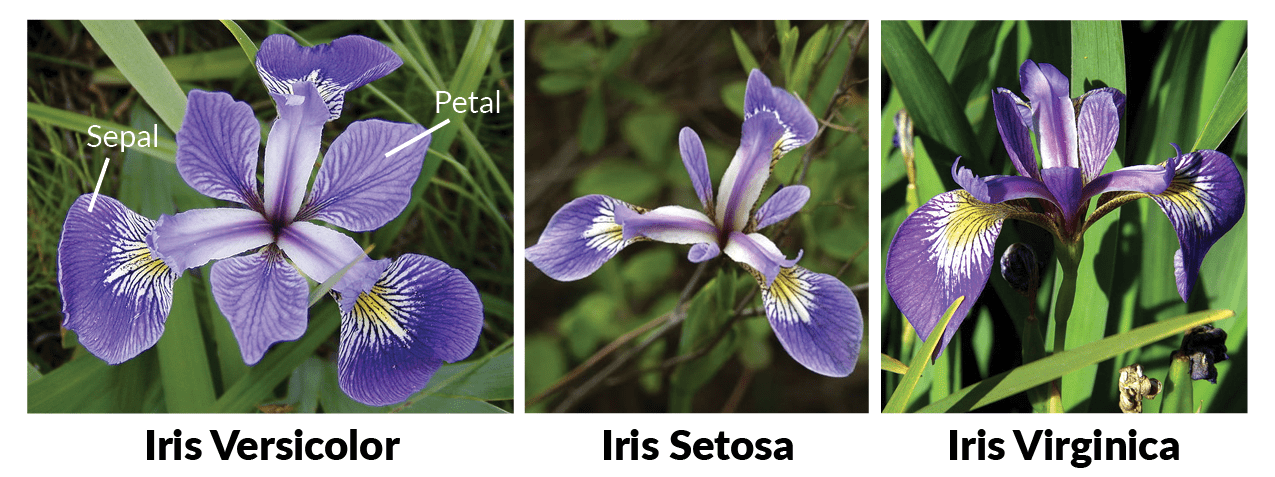
\includegraphics[width=\textwidth,height=1.5625in]{./img/iris-setosa.png}
\caption{Iris Arten}
\end{figure}

\begin{itemize}
\tightlist
\item
  Remember the \texttt{iris} data set?

  \begin{itemize}
  \tightlist
  \item
    contains information on iris flowers of different species
  \end{itemize}
\end{itemize}

\begin{Shaded}
\begin{Highlighting}[]
\FunctionTok{glimpse}\NormalTok{(iris)}
\end{Highlighting}
\end{Shaded}

\begin{verbatim}
## Rows: 150
## Columns: 5
## $ Sepal.Length <dbl> 5.1, 4.9, 4.7, 4.6, 5.0, 5.4, 4.6, 5.0, 4.4, 4.9, 5.4, 4.~
## $ Sepal.Width  <dbl> 3.5, 3.0, 3.2, 3.1, 3.6, 3.9, 3.4, 3.4, 2.9, 3.1, 3.7, 3.~
## $ Petal.Length <dbl> 1.4, 1.4, 1.3, 1.5, 1.4, 1.7, 1.4, 1.5, 1.4, 1.5, 1.5, 1.~
## $ Petal.Width  <dbl> 0.2, 0.2, 0.2, 0.2, 0.2, 0.4, 0.3, 0.2, 0.2, 0.1, 0.2, 0.~
## $ Species      <fct> setosa, setosa, setosa, setosa, setosa, setosa, setosa, s~
\end{verbatim}

\subsection{Imagine\ldots{}}\label{imagine}

\begin{itemize}
\tightlist
\item
  We only want data from species ``virginica''
\item
  We are interested in in sepal length
\item
  We want to adjust variable names
\end{itemize}

\subsection{First Example}\label{first-example}

\begin{Shaded}
\begin{Highlighting}[]
\NormalTok{iris\_virginica }\OtherTok{\textless{}{-}}\NormalTok{ iris }\SpecialCharTok{\%\textgreater{}\%} \CommentTok{\# 1. create new data set as copy}
  \FunctionTok{filter}\NormalTok{(Species }\SpecialCharTok{==} \StringTok{"virginica"}\NormalTok{) }\SpecialCharTok{\%\textgreater{}\%} \CommentTok{\# 2. only virginica}
  \FunctionTok{select}\NormalTok{(Petal.Length, Species)  }\SpecialCharTok{\%\textgreater{}\%} \CommentTok{\# 3. select columns }
  \FunctionTok{rename}\NormalTok{(}\AttributeTok{plength =}\NormalTok{ Petal.Length) }\CommentTok{\# 4. rename variable/column}

\FunctionTok{head}\NormalTok{(iris\_virginica)}
\end{Highlighting}
\end{Shaded}

\begin{verbatim}
##   plength   Species
## 1     6.0 virginica
## 2     5.1 virginica
## 3     5.9 virginica
## 4     5.6 virginica
## 5     5.8 virginica
## 6     6.6 virginica
\end{verbatim}

\begin{Shaded}
\begin{Highlighting}[]
\FunctionTok{str}\NormalTok{(iris\_virginica)}
\end{Highlighting}
\end{Shaded}

\begin{verbatim}
## 'data.frame':    50 obs. of  2 variables:
##  $ plength: num  6 5.1 5.9 5.6 5.8 6.6 4.5 6.3 5.8 6.1 ...
##  $ Species: Factor w/ 3 levels "setosa","versicolor",..: 3 3 3 3 3 3 3 3 3 3 ...
\end{verbatim}

\subsection{Filter}\label{filter}

\begin{figure}
\centering
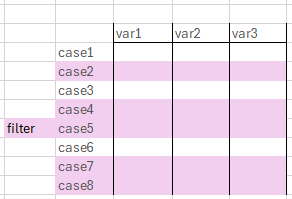
\includegraphics[width=\textwidth,height=1.04167in]{./img/filter.png}
\caption{filter scheme}
\end{figure}

\begin{itemize}
\tightlist
\item
  Filters data by a \textbf{value in a variable}

  \begin{itemize}
  \tightlist
  \item
    With filter we \textbf{keep only certain rows} in our data
  \end{itemize}
\item
  Needs \textbf{logical operators} as input

  \begin{itemize}
  \tightlist
  \item
    ``keep only cases where variable x has value abc''
  \item
    Can also be used with the ! to drop certain cases
  \item
    Drop NAs: \texttt{data\ \%\textgreater{}\%\ filter(!is.na(variable))}
  \end{itemize}
\end{itemize}

\subsection{Select}\label{select}

\begin{figure}
\centering
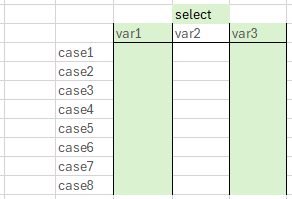
\includegraphics[width=\textwidth,height=1.04167in]{./img/select.png}
\caption{select scheme}
\end{figure}

\begin{itemize}
\tightlist
\item
  Selects \textbf{variables based on their names}

  \begin{itemize}
  \tightlist
  \item
    With select we \textbf{keep only certain columns} in our data
  \end{itemize}
\item
  Needs \textbf{variable names} as input

  \begin{itemize}
  \tightlist
  \item
    ``keep only variables with this name''
  \item
    Can also be used with the ! to drop certain variables
  \end{itemize}
\item
  Cave: if we want to extract one variable to calculate something, you will want to use \texttt{pull()} instead

  \begin{itemize}
  \tightlist
  \item
    Check \texttt{iris\ \%\textgreater{}\%\ select(Species)\ \%\textgreater{}\%\ class()} and \texttt{iris\ \%\textgreater{}\%\ pull(Species)\ \%\textgreater{}\%\ class()}
  \end{itemize}
\end{itemize}

\subsection{Mutate}\label{mutate}

\begin{itemize}
\tightlist
\item
  We also want the species to be capitalized in our data
\item
  We also want to add a new binary variable for whether a flower's petals are longer than 5.5 cm (1) or not (0)

  \begin{itemize}
  \tightlist
  \item
    for this, we use the \texttt{ifelse()} function:
  \item
    Needs a logical as first input, then what to do if it's true, last what to do if it's false
  \end{itemize}
\item
  Mutate takes a \textbf{variable name as input} (existing or new) and some \textbf{function or calculation} to be done on that variable
\end{itemize}

\begin{Shaded}
\begin{Highlighting}[]
\NormalTok{iris\_virginica }\OtherTok{\textless{}{-}}\NormalTok{ iris\_virginica }\SpecialCharTok{\%\textgreater{}\%} 
  \FunctionTok{mutate}\NormalTok{(}\AttributeTok{Species =} \FunctionTok{toupper}\NormalTok{(Species),}
         \AttributeTok{bigboi =} \FunctionTok{ifelse}\NormalTok{(plength }\SpecialCharTok{\textgreater{}} \FloatTok{5.5}\NormalTok{, }\DecValTok{1}\NormalTok{, }\DecValTok{0}\NormalTok{))}
\FunctionTok{head}\NormalTok{(iris\_virginica)}
\end{Highlighting}
\end{Shaded}

\begin{verbatim}
##   plength   Species bigboi
## 1     6.0 VIRGINICA      1
## 2     5.1 VIRGINICA      0
## 3     5.9 VIRGINICA      1
## 4     5.6 VIRGINICA      1
## 5     5.8 VIRGINICA      1
## 6     6.6 VIRGINICA      1
\end{verbatim}

\begin{Shaded}
\begin{Highlighting}[]
\FunctionTok{table}\NormalTok{(iris\_virginica}\SpecialCharTok{$}\NormalTok{Species)}
\end{Highlighting}
\end{Shaded}

\begin{verbatim}
## 
## VIRGINICA 
##        50
\end{verbatim}

\section{Exercise}\label{exercise-3}

Imagine we want to edit the iris data set for our american colleagues, who are interested in the petal width of the \textbf{setosa} and \textbf{versicolor} species.

\begin{enumerate}
\def\labelenumi{\arabic{enumi}.}
\tightlist
\item
  Create a new dataset from \texttt{iris} with a meaningful name
\item
  \texttt{select()} the variables of interest
\item
  \texttt{filter()} the species that we want

  \begin{itemize}
  \tightlist
  \item
    Use \%in\% to filter by more than one value, or think about a reverse approach\ldots!
  \end{itemize}
\item
  \texttt{rename()} the Petal.Width variable to be named pwidth
\item
  Use \texttt{mutate()} to add a new variable named ``pwidth\_inch'', which contains the petal width in inches

  \begin{itemize}
  \tightlist
  \item
    Calculation: pwidth / 2.54 (2.54 cm = 1 inch)
  \end{itemize}
\end{enumerate}

\subsection{Solution}\label{solution-3}

\begin{Shaded}
\begin{Highlighting}[]
\NormalTok{iris\_twospec }\OtherTok{\textless{}{-}}\NormalTok{ iris }\SpecialCharTok{\%\textgreater{}\%} 
  \FunctionTok{select}\NormalTok{(Petal.Width, Species) }\SpecialCharTok{\%\textgreater{}\%} 
  \FunctionTok{filter}\NormalTok{(Species }\SpecialCharTok{\%in\%} \FunctionTok{c}\NormalTok{(}\StringTok{"setosa"}\NormalTok{, }\StringTok{"versicolor"}\NormalTok{)) }\SpecialCharTok{\%\textgreater{}\%} 
  \CommentTok{\# or: filter(Species != "virginica")}
  \CommentTok{\# or: filter(Species == c("setosa" | "versicolor"))}
  \FunctionTok{rename}\NormalTok{(}\AttributeTok{pwidth =}\NormalTok{ Petal.Width) }\SpecialCharTok{\%\textgreater{}\%} 
  \FunctionTok{mutate}\NormalTok{(}\AttributeTok{pwidth\_inch =}\NormalTok{ pwidth }\SpecialCharTok{/} \FloatTok{2.54}\NormalTok{)}

\FunctionTok{head}\NormalTok{(iris\_twospec, }\DecValTok{8}\NormalTok{)}
\end{Highlighting}
\end{Shaded}

\begin{verbatim}
##   pwidth Species pwidth_inch
## 1    0.2  setosa  0.07874016
## 2    0.2  setosa  0.07874016
## 3    0.2  setosa  0.07874016
## 4    0.2  setosa  0.07874016
## 5    0.2  setosa  0.07874016
## 6    0.4  setosa  0.15748031
## 7    0.3  setosa  0.11811024
## 8    0.2  setosa  0.07874016
\end{verbatim}

\begin{figure}
\centering

\includegraphics{./img/hadley-meme.webp}
\caption{Hadley Wickham}
\end{figure}

Hadley Wickham, developer of the tidyverse

\section{\texorpdfstring{On a Tangent: \texttt{magrittr} pipe \%\textgreater\%}{On a Tangent: magrittr pipe \%\textgreater\%}}\label{on-a-tangent-magrittr-pipe}

\begin{itemize}
\tightlist
\item
  The pipe keeps our code readable and tidy
\item
  It allows us to keep edits in separate lines, but we still only have to run one command for every task we need
\item
  It's easy to add new commands by using another pipe operator, or to leave edits out but commenting out the respective line of code
\item
  Most things can be achieved with or without pipe
\end{itemize}

\subsection{Example}\label{example}

\begin{Shaded}
\begin{Highlighting}[]
\CommentTok{\# With pipe {-} clear}
\NormalTok{iris\_edit }\OtherTok{\textless{}{-}}\NormalTok{ iris }\SpecialCharTok{\%\textgreater{}\%}
 \FunctionTok{filter}\NormalTok{(Petal.Length }\SpecialCharTok{\textgreater{}} \DecValTok{3}\NormalTok{) }\SpecialCharTok{\%\textgreater{}\%} \CommentTok{\# only big petals}
 \FunctionTok{select}\NormalTok{(Species, Petal.Length, Sepal.Length) }\SpecialCharTok{\%\textgreater{}\%}  \CommentTok{\# only those columns}
 \FunctionTok{mutate}\NormalTok{(}\AttributeTok{random\_calculation =}\NormalTok{ Petal.Length }\SpecialCharTok{*}\NormalTok{ Sepal.Length) }\CommentTok{\# calculate random new variable}

\CommentTok{\# Without pipe {-} a lot of typing, prone to error, annoying to debug}
\NormalTok{iris\_edit2 }\OtherTok{\textless{}{-}} \FunctionTok{filter}\NormalTok{(iris, Petal.Length }\SpecialCharTok{\textgreater{}} \DecValTok{3}\NormalTok{)}
\NormalTok{iris\_edit2 }\OtherTok{\textless{}{-}} \FunctionTok{select}\NormalTok{(iris\_edit2, Species, Petal.Length, Sepal.Length)}
\NormalTok{iris\_edit2 }\OtherTok{\textless{}{-}} \FunctionTok{mutate}\NormalTok{(iris\_edit2, }\AttributeTok{random\_calculation =}\NormalTok{ Petal.Length }\SpecialCharTok{*}\NormalTok{ Sepal.Length)}

\CommentTok{\# Are the two versions equal?}
\FunctionTok{all.equal}\NormalTok{(iris\_edit, iris\_edit2)}
\end{Highlighting}
\end{Shaded}

\begin{verbatim}
## [1] TRUE
\end{verbatim}

\subsection{\texorpdfstring{Brainteaser }{Brainteaser }}\label{brainteaser-1}

\begin{itemize}
\item
  In the part with pipe we used the \texttt{iris} data to edit and assigned it to \texttt{iris\_edit}
\item
  In the part without pipe we used \texttt{iris} in the first line, but afterwards we used \texttt{iris\_edit2} for assignment and edit
\item
  Why is that?
\end{itemize}

\subsection{How to pipe for base-R}\label{how-to-pipe-for-base-r}

\begin{itemize}
\item
  Pipe helps us not to drown in parentheses when conducting analyses, e.g.~calculating a mean after filtering

  \begin{itemize}
  \tightlist
  \item
    It makes code longer but still easier to read
  \end{itemize}
\item
\begin{Shaded}
\begin{Highlighting}[]
\CommentTok{\# Without pipe}
\FunctionTok{round}\NormalTok{(}\FunctionTok{mean}\NormalTok{(iris}\SpecialCharTok{$}\NormalTok{Petal.Length[iris}\SpecialCharTok{$}\NormalTok{Species }\SpecialCharTok{==} \StringTok{"setosa"}\NormalTok{]), }\AttributeTok{digits =} \DecValTok{2}\NormalTok{)}
\end{Highlighting}
\end{Shaded}

\begin{verbatim}
## [1] 1.46
\end{verbatim}
\item
\begin{Shaded}
\begin{Highlighting}[]
\CommentTok{\# With pipe}
\NormalTok{iris }\SpecialCharTok{\%\textgreater{}\%} 
\FunctionTok{filter}\NormalTok{(Species }\SpecialCharTok{==} \StringTok{"setosa"}\NormalTok{) }\SpecialCharTok{\%\textgreater{}\%} 
\FunctionTok{pull}\NormalTok{(Petal.Length) }\SpecialCharTok{\%\textgreater{}\%}
\FunctionTok{mean}\NormalTok{() }\SpecialCharTok{\%\textgreater{}\%} \FunctionTok{round}\NormalTok{(}\AttributeTok{digits =} \DecValTok{2}\NormalTok{)}
\end{Highlighting}
\end{Shaded}

\begin{verbatim}
## [1] 1.46
\end{verbatim}
\end{itemize}

\subsection{\texorpdfstring{Brainteaser }{Brainteaser }}\label{brainteaser-2}

We want to edit the iris data to rename a Petal.Length to pl and mutate it to be multiplied by ten.

Why does the first version work, but not the second one?

\begin{Shaded}
\begin{Highlighting}[]
\CommentTok{\# Version 1}
\NormalTok{iris }\SpecialCharTok{\%\textgreater{}\%} 
  \FunctionTok{mutate}\NormalTok{(}\AttributeTok{Petal.Length =}\NormalTok{ Petal.Length }\SpecialCharTok{*} \DecValTok{10}\NormalTok{) }\SpecialCharTok{\%\textgreater{}\%} 
  \FunctionTok{rename}\NormalTok{(}\AttributeTok{pl =}\NormalTok{ Petal.Length) }\SpecialCharTok{\%\textgreater{}\%} 
  \FunctionTok{glimpse}\NormalTok{()}

\CommentTok{\# Version 2}
\NormalTok{iris }\SpecialCharTok{\%\textgreater{}\%} 
  \FunctionTok{rename}\NormalTok{(}\AttributeTok{pl =}\NormalTok{ Petal.Length) }\SpecialCharTok{\%\textgreater{}\%} 
  \FunctionTok{mutate}\NormalTok{(}\AttributeTok{Petal.Length =}\NormalTok{ Petal.Length }\SpecialCharTok{*} \DecValTok{10}\NormalTok{) }\SpecialCharTok{\%\textgreater{}\%} 
  \FunctionTok{glimpse}\NormalTok{()}
\end{Highlighting}
\end{Shaded}

\section{group\_by \& summarize}\label{group_by-summarize}

\begin{itemize}
\tightlist
\item
  With the dplyr-workflow, we can easily output group statistics
\item
  Keywords: \textbf{group\_by()} \& \textbf{summarize()}
\item
  The code is built like any other dplyr workflow with pipes ( \%\textgreater\% ) in between each:

  \begin{enumerate}
  \def\labelenumi{\arabic{enumi}.}
  \tightlist
  \item
    Define/ name the data frame
  \item
    group\_by(\emph{variable\_name})
  \item
    in summarize, define a name for the statistic, use a =, use a function like mean() for the measure
  \end{enumerate}
\end{itemize}

\subsection{Example: group\_by \& summarize}\label{example-group_by-summarize}

\begin{Shaded}
\begin{Highlighting}[]
\FunctionTok{names}\NormalTok{(Orange) }\CommentTok{\# use different default data set}
\end{Highlighting}
\end{Shaded}

\begin{verbatim}
## [1] "Tree"          "age"           "circumference"
\end{verbatim}

\begin{Shaded}
\begin{Highlighting}[]
\NormalTok{Orange }\SpecialCharTok{\%\textgreater{}\%} 
  \FunctionTok{group\_by}\NormalTok{(Tree) }\SpecialCharTok{\%\textgreater{}\%} 
  \FunctionTok{summarize}\NormalTok{(}\AttributeTok{m\_age =} \FunctionTok{mean}\NormalTok{(age),}
            \AttributeTok{m\_circumference =} \FunctionTok{mean}\NormalTok{(circumference),}
            \AttributeTok{n =} \FunctionTok{n}\NormalTok{())}
\end{Highlighting}
\end{Shaded}

\begin{verbatim}
## # A tibble: 5 x 4
##   Tree  m_age m_circumference     n
##   <ord> <dbl>           <dbl> <int>
## 1 3      922.            94       7
## 2 1      922.            99.6     7
## 3 5      922.           111.      7
## 4 2      922.           135.      7
## 5 4      922.           139.      7
\end{verbatim}

\subsection{Exercise: group\_by \& summarize}\label{exercise-group_by-summarize}

Follow the structure to group the iris data set by Species and output a summary with the mean values of all four other variables in the data.
Also include the grouped n.

\subsection{Solution}\label{solution-4}

\begin{Shaded}
\begin{Highlighting}[]
\NormalTok{iris }\SpecialCharTok{\%\textgreater{}\%} 
  \FunctionTok{group\_by}\NormalTok{(Species) }\SpecialCharTok{\%\textgreater{}\%} 
  \FunctionTok{summarize}\NormalTok{(}\AttributeTok{m\_plength =} \FunctionTok{mean}\NormalTok{(Petal.Length),}
            \AttributeTok{m\_pwidth =} \FunctionTok{mean}\NormalTok{(Petal.Width),}
            \AttributeTok{m\_slength =} \FunctionTok{mean}\NormalTok{(Sepal.Length),}
            \AttributeTok{m\_swidth =} \FunctionTok{mean}\NormalTok{(Sepal.Width),}
            \AttributeTok{n =} \FunctionTok{n}\NormalTok{())}
\end{Highlighting}
\end{Shaded}

\begin{verbatim}
## # A tibble: 3 x 6
##   Species    m_plength m_pwidth m_slength m_swidth     n
##   <fct>          <dbl>    <dbl>     <dbl>    <dbl> <int>
## 1 setosa          1.46    0.246      5.01     3.43    50
## 2 versicolor      4.26    1.33       5.94     2.77    50
## 3 virginica       5.55    2.03       6.59     2.97    50
\end{verbatim}

\section{Wrap-Up \& Further Resources}\label{wrap-up-further-resources-2}

Packages make working with R easier

\texttt{dplyr} is a powerful tool for editing data (\emph{select, filter, mutate\ldots{}})

The pipe \%\textgreater\% makes your code clearer and ``follows the thought process''

\href{https://r4ds.hadley.nz/}{R for Data Science} Book

\href{https://dplyr.tidyverse.org/}{dplyr vignette}

\href{https://www.youtube.com/watch?v=npOf6aXdguY&ab_channel=RichardOnData}{YouTube: 20 R Packages that you should know} - you for sure don't need them all, but there are some nice inspirations for working with packages in there

\begin{figure}
\centering

\includegraphics[width=\textwidth,height=4.16667in]{./img/idiotic.png}
\caption{Which idiot\ldots{}}\label{id}
\end{figure}

\chapter{Working with existing Data}\label{working-with-existing-data}

Please also install the \emph{wobblynameR} package (only available on GitHub). For that you need the \emph{devtools} package first:

\begin{enumerate}
\def\labelenumi{\arabic{enumi}.}
\tightlist
\item
  install.packages(``devtools'')
\item
  devtools::install\_github(``the-tave/wobblynameR'')
\end{enumerate}

\section{First Steps: Seminar Data}\label{first-steps-seminar-data}

\begin{itemize}
\tightlist
\item
  Download the data frame from ILIAS and save it in the data subfolder in your R-Project.
\item
  Use the ``Import Dataset'' Menu under the \emph{Environment} tab 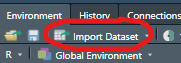
\includegraphics[width=\textwidth,height=0.41667in]{./img/import_dataset.png}

  \begin{itemize}
  \tightlist
  \item
    In that menu, we can select our data file \& choose some basic aspects of reading in that data
  \end{itemize}
\end{itemize}

Make sure you have the right package installed for reading in specific data types! Here: Please install the readr package with install.packages(``readr'')

\subsection{Reading in the data}\label{reading-in-the-data}

\subsubsection{Generated Code}\label{generated-code}

\begin{Shaded}
\begin{Highlighting}[]
\FunctionTok{library}\NormalTok{(readr)}
\NormalTok{PsychResearchR\_data }\OtherTok{\textless{}{-}} \FunctionTok{read\_delim}\NormalTok{(}\StringTok{"data/PsychResearchR\_data.csv"}\NormalTok{, }
    \AttributeTok{delim =} \StringTok{";"}\NormalTok{, }\AttributeTok{escape\_double =} \ConstantTok{FALSE}\NormalTok{, }\AttributeTok{trim\_ws =} \ConstantTok{TRUE}\NormalTok{)}
\FunctionTok{View}\NormalTok{(PsychResearchR\_data)}
\end{Highlighting}
\end{Shaded}

\subsection{\texorpdfstring{Basic Edits }{Basic Edits }}\label{basic-edits}

\begin{enumerate}
\def\labelenumi{\arabic{enumi}.}
\tightlist
\item
  Choose an appropriate name, e.g.~\texttt{raw}
\item
  Put all \emph{library commands} at the top of the script so you are ready to conduct all analyses
\item
  You do not need the \emph{View()} command in your script
\item
  If you are not sure about the state of your data, look at it first!

  \begin{itemize}
  \tightlist
  \item
    View() opens the whole data in new tab; glimpse(), str() and head() give you a rough overview; names() shows you all variable names
  \end{itemize}
\item
  Some edits are already possible in the menu! Column types can (and sometimes should) be adjusted, e.g.~recognizing dates
\item
  Create a new dataset as a copy in which you do all further edits! E.g. \texttt{seminar} with proper varname prefix
\end{enumerate}

\subsection{\texorpdfstring{Basic Edits }{Basic Edits }}\label{basic-edits-1}

\subsubsection{Result}\label{result}

\begin{Shaded}
\begin{Highlighting}[]
\FunctionTok{library}\NormalTok{(readr)}
\FunctionTok{library}\NormalTok{(wobblynameR)}

\NormalTok{raw }\OtherTok{\textless{}{-}} \FunctionTok{read\_delim}\NormalTok{(}\StringTok{"./data/PsychResearchR\_data.csv"}\NormalTok{, }
    \AttributeTok{delim =} \StringTok{";"}\NormalTok{, }\AttributeTok{escape\_double =} \ConstantTok{FALSE}\NormalTok{, }
    \AttributeTok{col\_types =} \FunctionTok{cols}\NormalTok{(}\AttributeTok{.wx.5.start\_date =} \FunctionTok{col\_date}\NormalTok{(}\AttributeTok{format =} \StringTok{"\%m/\%d/\%y"}\NormalTok{),}
                     \AttributeTok{.wx.7.end\_date =} \FunctionTok{col\_date}\NormalTok{(}\AttributeTok{format =} \StringTok{"\%m/\%d/\%y"}\NormalTok{), }
                     \AttributeTok{...32 =} \FunctionTok{col\_skip}\NormalTok{()),}
    \AttributeTok{trim\_ws =} \ConstantTok{TRUE}\NormalTok{)}
\end{Highlighting}
\end{Shaded}

\begin{verbatim}
## New names:
## * `` -> `...32`
\end{verbatim}

\begin{Shaded}
\begin{Highlighting}[]
\CommentTok{\# Add "v" as varname prefix to all variables}
\NormalTok{seminar }\OtherTok{\textless{}{-}} \FunctionTok{namepref0}\NormalTok{(raw, }\StringTok{"v"}\NormalTok{)}
\end{Highlighting}
\end{Shaded}

\subsection{Choosing how to read in the data}\label{choosing-how-to-read-in-the-data}

\begin{longtable}[]{@{}ll@{}}
\toprule\noalign{}
Data Source & R command \\
\midrule\noalign{}
\endhead
\bottomrule\noalign{}
\endlastfoot
WEXTOR (CSV) & \texttt{readr::read\_delim("data.csv",\ delim\ =\ ";")} \\
Excel (XLSX) & \texttt{xlsx::read.xlsx("data.xlsx",\ sheetIndex\ =\ 1)} \\
R Data Source (RDS) & \texttt{readRDS("data.Rds")} \\
SPSS (SAV) & \texttt{foreign::read.spss("data.sav")} \\
\end{longtable}

\section{\texorpdfstring{Working with the data: Codebook}{Working with the data:   Codebook}}\label{working-with-the-data-codebook}

\begin{itemize}
\tightlist
\item
  What variables are in the data? -\textgreater{} \texttt{names(seminar)}

  \begin{itemize}
  \tightlist
  \item
    v.wx.1.id, v.wx.2.ip, v.wx.3.experimental\_condition, v.wx.4.start\_time, v.wx.5.start\_date, v.wx.6.end\_time, v.wx.7.end\_date, v.wx.8.session\_length, v.wx.page\_trail, v.wx.pages\_visited, v.wx.user\_agent, v01\_gender, v02\_age, v03\_prog\_exp, v04\_bodyheight, v05\_skill\_tech, v06\_loc, v07\_genre, v08\_loudness, v09\_smoke, v10\_motivation, v11\_soul, v12\_soul\_phil, vrt\_1, vrt\_2, vrt\_3, vvi\_1, vvi\_2, vvi\_3, vz0\_browser\_screen\_h, vz0\_browser\_screen\_w
  \end{itemize}
\item
  What can they tell us? Which analyses might be of interest?
\end{itemize}

\section{\texorpdfstring{Working with the data: Descriptives}{Working with the data:   Descriptives}}\label{working-with-the-data-descriptives}

\begin{itemize}
\tightlist
\item
  In any report, we need to give our readers/ listeners/\ldots{} an overview of the data

  \begin{itemize}
  \tightlist
  \item
    We need to know the sample to judge the results!
  \item
    A sample of e.g.~10 female psychology students probably shows different results -generally speaking - than a sample of 10 male soldiers
  \end{itemize}
\item
  What are descriptives?

  \begin{itemize}
  \tightlist
  \item
    Mean
  \item
    Median
  \item
    Mode
  \item
    Variability (standard deviation)
  \item
    Data Visualization\ldots{}
  \end{itemize}
\end{itemize}

\subsection{group\_by \& summarize}\label{group_by-summarize-1}

\begin{itemize}
\tightlist
\item
  With the dplyr-workflow, we can easily output group statistics
\item
  Keywords: \textbf{group\_by()} \& \textbf{summarize()}
\item
  The code is built like any other dplyr workflow with pipes ( \%\textgreater\% ) in between each:

  \begin{enumerate}
  \def\labelenumi{\arabic{enumi}.}
  \tightlist
  \item
    Define/ name the data frame
  \item
    group\_by(\emph{variable\_name})
  \item
    in summarize, define a name for the statistic, use a =, use a function like mean() for the measure
  \end{enumerate}
\end{itemize}

\subsection{Example: group\_by \& summarize}\label{example-group_by-summarize-1}

\begin{Shaded}
\begin{Highlighting}[]
\NormalTok{iris }\SpecialCharTok{\%\textgreater{}\%} 
  \FunctionTok{group\_by}\NormalTok{(Species) }\SpecialCharTok{\%\textgreater{}\%} 
  \FunctionTok{summarize}\NormalTok{(}\AttributeTok{m\_plength =} \FunctionTok{mean}\NormalTok{(Petal.Length),}
            \AttributeTok{med\_pwidth =} \FunctionTok{median}\NormalTok{(Petal.Width),}
            \AttributeTok{m\_slength =} \FunctionTok{mean}\NormalTok{(Sepal.Length),}
            \AttributeTok{mode\_swidth =} \FunctionTok{getmode}\NormalTok{(Sepal.Width),}
            \AttributeTok{n =} \FunctionTok{n}\NormalTok{())}
\end{Highlighting}
\end{Shaded}

\begin{verbatim}
## # A tibble: 3 x 6
##   Species    m_plength med_pwidth m_slength mode_swidth     n
##   <fct>          <dbl>      <dbl>     <dbl>       <dbl> <int>
## 1 setosa          1.46        0.2      5.01         3.4    50
## 2 versicolor      4.26        1.3      5.94         3      50
## 3 virginica       5.55        2        6.59         3      50
\end{verbatim}

\subsection{Exercise: group\_by \& summarize}\label{exercise-group_by-summarize-1}

Follow the structure to group the edited seminar data by belief in the soul and output a summary with

\begin{itemize}
\tightlist
\item
  mean age
\item
  mean technological skill
\item
  mode music genre
\item
  median volume of music
\item
  grouped n (function \emph{n()})
\end{itemize}

\subsection{Solution}\label{solution-5}

\begin{Shaded}
\begin{Highlighting}[]
\NormalTok{seminar }\SpecialCharTok{\%\textgreater{}\%} 
  \FunctionTok{group\_by}\NormalTok{(v11\_soul) }\SpecialCharTok{\%\textgreater{}\%} 
  \FunctionTok{summarize}\NormalTok{(}\AttributeTok{m\_age =} \FunctionTok{mean}\NormalTok{(v02\_age),}
            \AttributeTok{m\_tech\_skill =} \FunctionTok{mean}\NormalTok{(v05\_skill\_tech),}
            \AttributeTok{mode\_music =} \FunctionTok{getmode}\NormalTok{(v07\_genre),}
            \AttributeTok{median\_volume =} \FunctionTok{median}\NormalTok{(v08\_loudness),}
            \AttributeTok{n =} \FunctionTok{n}\NormalTok{())}
\end{Highlighting}
\end{Shaded}

\begin{verbatim}
## # A tibble: 3 x 6
##   v11_soul m_age m_tech_skill mode_music median_volume     n
##   <chr>    <dbl>        <dbl> <chr>              <dbl> <int>
## 1 dunno     23.4         29.4 techno              89       5
## 2 no        22           45   pop                 74.5     2
## 3 yes       22.5         42   rock                67.5     6
\end{verbatim}

\section{Wrap-Up \& Further Resources}\label{wrap-up-further-resources-3}

Reading in data works with commands like readRDS() but also the ``Import Dataset'' Menu

Use the menu for WEXTOR data to get an overview and reproducible code

Get/ create a codebook for your data

Always report descriptive data

dplyr's \texttt{group\_by()} and \texttt{summarize()} can output grouped descriptives

\href{https://www.datafiles.samhsa.gov/get-help/format-specific-issues/how-do-i-read-data-r}{Reading in Data in Different Formats}

\href{https://statsandr.com/blog/descriptive-statistics-in-r/}{Stats and R: Descriptives}

\chapter{Loops and Conditionals}\label{loops-and-conditionals}

\section{What is a loop?}\label{what-is-a-loop}

\begin{itemize}
\tightlist
\item
  Loops are automations that take care of repetitive tasks

  \begin{itemize}
  \tightlist
  \item
    Typically, we might go through data row by row and perform a task
  \end{itemize}
\item
  Loops can have different forms:

  \begin{itemize}
  \tightlist
  \item
    \textbf{for}: loop over a pre-defined set of values, such as a number sequence
  \item
    \textbf{while}: define constraints and keep loop running as long as they are met
  \item
    \textbf{repeat}: loop repeats until broken (\emph{I do not recommend this ever!})
  \end{itemize}
\item
  For is most common, while is nice for more advanced simulations
\end{itemize}

\subsection{What are conditionals?}\label{what-are-conditionals}

\begin{itemize}
\tightlist
\item
  Conditionals define different actions for different conditions
\item
  They follow intuitive language:

  \begin{itemize}
  \tightlist
  \item
    \textbf{if}: define action to take when condition is met (logical)
  \item
    \textbf{else if}: defince action for another condition
  \item
    \textbf{else}: define action for everything else
  \end{itemize}
\item
  \textbf{ifelse} is the shortcut-function we already got to know for recoding with \texttt{mutate()}

  \begin{itemize}
  \tightlist
  \item
    defines exactly 1 condition, 1 action, 1 alternative
  \item
    expandable version of ifelse is case\_when
  \end{itemize}
\end{itemize}

\section{Exercise: What should I use?}\label{exercise-what-should-i-use}

\begin{enumerate}
\def\labelenumi{\arabic{enumi}.}
\tightlist
\item
  I want to print numbers from 1 to 7!

  \begin{itemize}
  \tightlist
  \item
    for loop (but realistically \emph{1:7} ;) )
  \end{itemize}
\item
  I need to simulate more data as long as my sample size is smaller than 200!

  \begin{itemize}
  \tightlist
  \item
    while loop
  \end{itemize}
\item
  I want to print the age of only the females in my sample!

  \begin{itemize}
  \tightlist
  \item
    if/ else
  \end{itemize}
\end{enumerate}

\section{for-loop}\label{for-loop}

\begin{itemize}
\tightlist
\item
  In a for loop, we need to define the range \emph{for} which the loop should run
\item
  We define an \emph{iterating variable} that will change each time the loop runs and take on all values of the defined range

  \begin{itemize}
  \tightlist
  \item
    Typically, we call this variable ``i''
  \end{itemize}
\item
  We define the range in round brackets and all actions the loop should take in curly brackets
\end{itemize}

\subsection{Example}\label{example-1}

\begin{Shaded}
\begin{Highlighting}[]
\ControlFlowTok{for}\NormalTok{(i }\ControlFlowTok{in} \DecValTok{1}\SpecialCharTok{:}\DecValTok{4}\NormalTok{)\{}
  \FunctionTok{print}\NormalTok{(}\FunctionTok{paste}\NormalTok{(}\StringTok{"The iteration is"}\NormalTok{, i))}
\NormalTok{\}}
\end{Highlighting}
\end{Shaded}

\begin{verbatim}
## [1] "The iteration is 1"
## [1] "The iteration is 2"
## [1] "The iteration is 3"
## [1] "The iteration is 4"
\end{verbatim}

\subsection{Conditionals: If - else}\label{conditionals-if---else}

\begin{Shaded}
\begin{Highlighting}[]
\ControlFlowTok{if}\NormalTok{(variable }\SpecialCharTok{==} \StringTok{"value"}\NormalTok{)\{}
  \FunctionTok{print}\NormalTok{(}\StringTok{"Do something"}\NormalTok{)}
\NormalTok{\} }\ControlFlowTok{else} \ControlFlowTok{if}\NormalTok{(variable }\SpecialCharTok{==} \StringTok{"other\_value"}\NormalTok{)\{}
  \FunctionTok{print}\NormalTok{(}\StringTok{"Do some other thing"}\NormalTok{)}
\NormalTok{\} }\ControlFlowTok{else}\NormalTok{ \{}
  \FunctionTok{print}\NormalTok{(}\StringTok{"Do anything else"}\NormalTok{)}
\NormalTok{\}}
\end{Highlighting}
\end{Shaded}

\subsection{Conditionals: If - else}\label{conditionals-if---else-1}

\subsubsection{Checking numbers \textbar{}}\label{checking-numbers}

We want to test whether numbers in a loop are divisible by 3. If they are, we will display ``Divisible by 3'', and if not, we will simply output the iteration number like before.

For that we will use the modulo \%\% , which gives us the rest of a division. Let's try it out!

\subsubsection{Checking numbers \textbar\textbar{}}\label{checking-numbers-1}

\begin{Shaded}
\begin{Highlighting}[]
\ControlFlowTok{for}\NormalTok{(i }\ControlFlowTok{in} \DecValTok{1}\SpecialCharTok{:}\DecValTok{4}\NormalTok{)\{}
  \ControlFlowTok{if}\NormalTok{(i }\SpecialCharTok{\%\%} \DecValTok{3} \SpecialCharTok{==} \DecValTok{0}\NormalTok{)\{}
    \FunctionTok{print}\NormalTok{(}\StringTok{"Divisible by 3!"}\NormalTok{)}
\NormalTok{  \} }\ControlFlowTok{else}\NormalTok{ \{}
    \FunctionTok{print}\NormalTok{(i) }
\NormalTok{  \}}
\NormalTok{\}}
\end{Highlighting}
\end{Shaded}

\begin{verbatim}
## [1] 1
## [1] 2
## [1] "Divisible by 3!"
## [1] 4
\end{verbatim}

\subsection{Exercise}\label{exercise-4}

Use a for-loop to display your favorite numbers.
The numbers should be between 10 and 25.

If the number is divisible completely by 5, you should output ``Divisible by 5!'', if not please output the iteration number only.

\subsection{Solution}\label{solution-6}

\begin{Shaded}
\begin{Highlighting}[]
\ControlFlowTok{for}\NormalTok{(i }\ControlFlowTok{in} \DecValTok{10}\SpecialCharTok{:}\DecValTok{25}\NormalTok{)\{}
  \ControlFlowTok{if}\NormalTok{(i }\SpecialCharTok{\%\%} \DecValTok{5} \SpecialCharTok{==} \DecValTok{0}\NormalTok{)\{}
    \FunctionTok{print}\NormalTok{(}\StringTok{"Divisible by 5!"}\NormalTok{)}
\NormalTok{  \} }\ControlFlowTok{else}\NormalTok{ \{}
    \FunctionTok{print}\NormalTok{(i) }
\NormalTok{  \}}
\NormalTok{\}}
\end{Highlighting}
\end{Shaded}

\begin{verbatim}
## [1] "Divisible by 5!"
## [1] 11
## [1] 12
## [1] 13
## [1] 14
## [1] "Divisible by 5!"
## [1] 16
## [1] 17
## [1] 18
## [1] 19
## [1] "Divisible by 5!"
## [1] 21
## [1] 22
## [1] 23
## [1] 24
## [1] "Divisible by 5!"
\end{verbatim}

\section{Same function, different variables}\label{same-function-different-variables}

\begin{Shaded}
\begin{Highlighting}[]
\ControlFlowTok{for}\NormalTok{(i }\ControlFlowTok{in} \FunctionTok{c}\NormalTok{(}\StringTok{"Sepal.Length"}\NormalTok{, }\StringTok{"Sepal.Width"}\NormalTok{, }\StringTok{"Petal.Length"}\NormalTok{, }\StringTok{"Petal.Width"}\NormalTok{))\{}
  \FunctionTok{print}\NormalTok{(}\FunctionTok{mean}\NormalTok{(iris[ , i]))}
\NormalTok{\}}
\end{Highlighting}
\end{Shaded}

\begin{verbatim}
## [1] 5.843333
## [1] 3.057333
## [1] 3.758
## [1] 1.199333
\end{verbatim}

Brainteaser : What is the class() of i here?

\begin{itemize}
\tightlist
\item
  character
\end{itemize}

\subsection{More sophisticated}\label{more-sophisticated}

\begin{Shaded}
\begin{Highlighting}[]
\NormalTok{vector }\OtherTok{\textless{}{-}} \FunctionTok{c}\NormalTok{(}\StringTok{"Sepal.Length"}\NormalTok{, }\StringTok{"Sepal.Width"}\NormalTok{, }\StringTok{"Petal.Length"}\NormalTok{, }\StringTok{"Petal.Width"}\NormalTok{)}

\ControlFlowTok{for}\NormalTok{(i }\ControlFlowTok{in} \DecValTok{1}\SpecialCharTok{:}\FunctionTok{length}\NormalTok{(vector))\{}
  \FunctionTok{print}\NormalTok{(}\FunctionTok{paste}\NormalTok{(}\StringTok{"The mean value of"}\NormalTok{, vector[i], }\StringTok{"is"}\NormalTok{, }
              \FunctionTok{round}\NormalTok{(}\FunctionTok{mean}\NormalTok{(iris[ , vector[i]]), }\DecValTok{2}\NormalTok{)))}
\NormalTok{\}}
\end{Highlighting}
\end{Shaded}

\begin{verbatim}
## [1] "The mean value of Sepal.Length is 5.84"
## [1] "The mean value of Sepal.Width is 3.06"
## [1] "The mean value of Petal.Length is 3.76"
## [1] "The mean value of Petal.Width is 1.2"
\end{verbatim}

Brainteaser : And what is the class() of i now?

\begin{itemize}
\tightlist
\item
  integer (numeric)
\end{itemize}

\subsection{With saving values}\label{with-saving-values}

\begin{Shaded}
\begin{Highlighting}[]
\NormalTok{vector }\OtherTok{\textless{}{-}} \FunctionTok{c}\NormalTok{(}\StringTok{"Sepal.Length"}\NormalTok{, }\StringTok{"Sepal.Width"}\NormalTok{, }\StringTok{"Petal.Length"}\NormalTok{, }\StringTok{"Petal.Width"}\NormalTok{)}
\NormalTok{means }\OtherTok{\textless{}{-}} \FunctionTok{rep}\NormalTok{(}\ConstantTok{NA}\NormalTok{, }\FunctionTok{length}\NormalTok{(vector)) }\CommentTok{\# create "empty" vector to fill}

\ControlFlowTok{for}\NormalTok{(i }\ControlFlowTok{in} \DecValTok{1}\SpecialCharTok{:}\FunctionTok{length}\NormalTok{(vector))\{}
  \FunctionTok{print}\NormalTok{(}\FunctionTok{paste}\NormalTok{(}\StringTok{"The mean value of"}\NormalTok{, vector[i], }\StringTok{"is"}\NormalTok{, }
              \FunctionTok{round}\NormalTok{(}\FunctionTok{mean}\NormalTok{(iris[ , vector[i]]), }\DecValTok{2}\NormalTok{)))}
\NormalTok{  means[i] }\OtherTok{\textless{}{-}} \FunctionTok{round}\NormalTok{(}\FunctionTok{mean}\NormalTok{(iris[ , vector[i]]), }\DecValTok{2}\NormalTok{)}
\NormalTok{\}}
\end{Highlighting}
\end{Shaded}

\begin{verbatim}
## [1] "The mean value of Sepal.Length is 5.84"
## [1] "The mean value of Sepal.Width is 3.06"
## [1] "The mean value of Petal.Length is 3.76"
## [1] "The mean value of Petal.Width is 1.2"
\end{verbatim}

\subsection{Exercise: Seminar Data}\label{exercise-seminar-data}

Please download an edited version of our seminar data from ILIAS. You will find it under \emph{data} as a zip folder. The dataset in it should have ``.Rds'' as a file ending. Read it in using:

\begin{Shaded}
\begin{Highlighting}[]
\NormalTok{seminar }\OtherTok{\textless{}{-}} \FunctionTok{readRDS}\NormalTok{(}\StringTok{"./data/seminar\_data.Rds"}\NormalTok{)}
\end{Highlighting}
\end{Shaded}

\textbf{Create a for-loop that saves the means of age, body height and technological skill from that seminar data in a vector named ``seminar\_means''.}

Hint: I renamed the variables to make them nicer to work with, so check out names(seminar)!

\subsection{Solution}\label{solution-7}

\begin{Shaded}
\begin{Highlighting}[]
\NormalTok{vector }\OtherTok{\textless{}{-}} \FunctionTok{c}\NormalTok{(}\StringTok{"v02\_age"}\NormalTok{, }\StringTok{"v04\_bodyheight"}\NormalTok{, }\StringTok{"v05\_skill\_tech"}\NormalTok{)}
\NormalTok{seminar\_means }\OtherTok{\textless{}{-}} \FunctionTok{rep}\NormalTok{(}\ConstantTok{NA}\NormalTok{, }\FunctionTok{length}\NormalTok{(vector)) }\CommentTok{\# create "empty" vector to fill}

\ControlFlowTok{for}\NormalTok{(i }\ControlFlowTok{in} \DecValTok{1}\SpecialCharTok{:}\FunctionTok{length}\NormalTok{(vector))\{}
\NormalTok{  seminar\_means[i] }\OtherTok{\textless{}{-}} \FunctionTok{round}\NormalTok{(}\FunctionTok{mean}\NormalTok{(seminar[ , vector[i]]), }\DecValTok{2}\NormalTok{)}
\NormalTok{\}}
\end{Highlighting}
\end{Shaded}

\subsection{Checking What's Going On}\label{checking-whats-going-on}

\subsubsection{browser()}\label{browser}

\begin{itemize}
\tightlist
\item
  In order to break our loop and enter a ``debugging'' mode, we can add browser() to any loop like so:
\end{itemize}

\begin{Shaded}
\begin{Highlighting}[]
\NormalTok{vector }\OtherTok{\textless{}{-}} \FunctionTok{c}\NormalTok{(}\StringTok{"v02\_age"}\NormalTok{, }\StringTok{"v04\_bodyheight"}\NormalTok{, }\StringTok{"v05\_skill\_tech"}\NormalTok{)}
\NormalTok{seminar\_means }\OtherTok{\textless{}{-}} \FunctionTok{rep}\NormalTok{(}\ConstantTok{NA}\NormalTok{, }\FunctionTok{length}\NormalTok{(vector)) }\CommentTok{\# create "empty" vector to fill}

\ControlFlowTok{for}\NormalTok{(i }\ControlFlowTok{in} \DecValTok{1}\SpecialCharTok{:}\FunctionTok{length}\NormalTok{(vector))\{}
\NormalTok{  seminar\_means[i] }\OtherTok{\textless{}{-}} \FunctionTok{round}\NormalTok{(}\FunctionTok{mean}\NormalTok{(seminar[ , vector[i]]), }\DecValTok{2}\NormalTok{)}
  \FunctionTok{browser}\NormalTok{()}
\NormalTok{\}}
\end{Highlighting}
\end{Shaded}

\begin{itemize}
\item
  The loop will run the first iteration until browser is called and then pause
\item
  It allows you to check in the console whether all variables look the way you want them to without having to wait for the loop to run

  \begin{itemize}
  \tightlist
  \item
    Or if there are errors/ warnings, you can check \emph{when} they occur by moving the browser() to a different location in the code
  \end{itemize}
\item
  To continue with the next iteration while in browser, type ``c'' into the console, ``Q'' to quit

  \begin{itemize}
  \tightlist
  \item
    The Esc key will also terminate the browser
  \end{itemize}
\item
  \textbf{Make sure you exit it} before continuing with anything else
\end{itemize}

\section{Loop with Conditional}\label{loop-with-conditional}

In our seminar data, the \textbf{average body height is 167.23 cm}. We want to create a loop that goes through all rows (all seminar students) and outputs their height and whether it is above or below average.

What do we need for that?

\subsection{Elements}\label{elements}

\begin{itemize}
\tightlist
\item
  For each person:
\item
  Check \emph{if} their body height is above average

  \begin{itemize}
  \tightlist
  \item
    If yes: Output ``This person is taller than average with \ldots{}''
  \item
    Else: Output ``This person is less tall than average with\ldots{}''
  \end{itemize}
\item
  Then paste the person's body height
\item
  Loop that over each person!
\end{itemize}

\subsection{Solution}\label{solution-8}

\begin{Shaded}
\begin{Highlighting}[]
\ControlFlowTok{for}\NormalTok{(i }\ControlFlowTok{in} \DecValTok{1}\SpecialCharTok{:}\FunctionTok{nrow}\NormalTok{(seminar))\{}
  \ControlFlowTok{if}\NormalTok{(seminar}\SpecialCharTok{$}\NormalTok{v04\_bodyheight[i] }\SpecialCharTok{\textgreater{}} \FunctionTok{mean}\NormalTok{(seminar}\SpecialCharTok{$}\NormalTok{v04\_bodyheight)) \{}
    \FunctionTok{print}\NormalTok{(}\FunctionTok{paste}\NormalTok{(}\StringTok{"This person is taller than average with"}\NormalTok{, seminar}\SpecialCharTok{$}\NormalTok{v04\_bodyheight[i], }\StringTok{"cm."}\NormalTok{))}
\NormalTok{  \} }\ControlFlowTok{else}\NormalTok{ \{}
    \FunctionTok{print}\NormalTok{(}\FunctionTok{paste}\NormalTok{(}\StringTok{"This person is less tall than average with"}\NormalTok{, seminar}\SpecialCharTok{$}\NormalTok{v04\_bodyheight[i], }\StringTok{"cm."}\NormalTok{))}
\NormalTok{  \}}
\NormalTok{\}}
\end{Highlighting}
\end{Shaded}

\begin{verbatim}
## [1] "This person is taller than average with 168 cm."
## [1] "This person is less tall than average with 160 cm."
## [1] "This person is taller than average with 171 cm."
## [1] "This person is less tall than average with 166 cm."
## [1] "This person is taller than average with 169 cm."
## [1] "This person is less tall than average with 164 cm."
## [1] "This person is less tall than average with 161 cm."
## [1] "This person is less tall than average with 166 cm."
## [1] "This person is taller than average with 183 cm."
## [1] "This person is taller than average with 172 cm."
## [1] "This person is less tall than average with 160 cm."
## [1] "This person is less tall than average with 164 cm."
## [1] "This person is taller than average with 170 cm."
\end{verbatim}

\subsection{And a more complicated outlook\ldots{}}\label{and-a-more-complicated-outlook}

\subsubsection{What happens here?}\label{what-happens-here}

\begin{Shaded}
\begin{Highlighting}[]
\ControlFlowTok{for}\NormalTok{(i }\ControlFlowTok{in} \DecValTok{1}\SpecialCharTok{:}\FunctionTok{nrow}\NormalTok{(seminar))\{}
  \ControlFlowTok{if}\NormalTok{(seminar}\SpecialCharTok{$}\NormalTok{v11\_soul[i] }\SpecialCharTok{==} \StringTok{"yes"}\NormalTok{)\{ }\CommentTok{\# Check soul belief}
\NormalTok{    text1 }\OtherTok{\textless{}{-}} \StringTok{"This person belives in the soul and"}
\NormalTok{  \} }\ControlFlowTok{else} \ControlFlowTok{if}\NormalTok{ (seminar}\SpecialCharTok{$}\NormalTok{v11\_soul[i] }\SpecialCharTok{==} \StringTok{"no"}\NormalTok{) \{}
\NormalTok{    text1 }\OtherTok{\textless{}{-}} \StringTok{"This person does not belive in the soul and"}
\NormalTok{  \} }\ControlFlowTok{else}\NormalTok{ \{ text1 }\OtherTok{\textless{}{-}} \StringTok{"This person is unsure about the soul and"}\NormalTok{ \}}
  
  \ControlFlowTok{if}\NormalTok{(seminar}\SpecialCharTok{$}\NormalTok{v12\_soul\_phil[i] }\SpecialCharTok{==} \StringTok{"monism"}\NormalTok{)\{  }\CommentTok{\# Check mind{-}body{-}philosophy}
\NormalTok{    text2 }\OtherTok{\textless{}{-}} \StringTok{"believes the m{-}b{-}relationship is monistic."}
\NormalTok{  \} }\ControlFlowTok{else} \ControlFlowTok{if}\NormalTok{ (seminar}\SpecialCharTok{$}\NormalTok{v12\_soul\_phil[i] }\SpecialCharTok{==} \StringTok{"dualism"}\NormalTok{) \{}
\NormalTok{    text2 }\OtherTok{\textless{}{-}} \StringTok{"believes the m{-}b{-}relationship is dualistic."}
\NormalTok{  \} }\ControlFlowTok{else}\NormalTok{ \{ text2 }\OtherTok{\textless{}{-}} \StringTok{"is unsure of the m{-}b{-}relationship."}\NormalTok{ \}}
  
  \FunctionTok{print}\NormalTok{(}\FunctionTok{paste}\NormalTok{(text1, text2)) }\CommentTok{\# Print text}
\NormalTok{\}}
\end{Highlighting}
\end{Shaded}

\subsection{Result}\label{result-1}

\begin{verbatim}
## [1] "This person belives in the soul and believes the m-b-relationship is dualistic."
## [1] "This person belives in the soul and is unsure of the m-b-relationship."
## [1] "This person belives in the soul and believes the m-b-relationship is monistic."
## [1] "This person is unsure about the soul and is unsure of the m-b-relationship."
## [1] "This person belives in the soul and is unsure of the m-b-relationship."
## [1] "This person does not belive in the soul and believes the m-b-relationship is monistic."
## [1] "This person is unsure about the soul and is unsure of the m-b-relationship."
## [1] "This person is unsure about the soul and is unsure of the m-b-relationship."
## [1] "This person does not belive in the soul and is unsure of the m-b-relationship."
## [1] "This person belives in the soul and believes the m-b-relationship is monistic."
## [1] "This person is unsure about the soul and believes the m-b-relationship is dualistic."
## [1] "This person belives in the soul and believes the m-b-relationship is dualistic."
## [1] "This person is unsure about the soul and is unsure of the m-b-relationship."
\end{verbatim}

\section{Wrap-Up \& Further Resources}\label{wrap-up-further-resources-4}

For-Loops must have a defined sequence to run over, e.g.~1 to 4

For-loops are the most common in R and are fit for most tasks

Loops are a powerful tool to e.g.~easily perform the same task many times

Conditionals give you control over different operations depending on your data

In combination, loops and conditionals are most useful

Don't forget to play and create fun loops!

\href{https://www.w3schools.com/r/r_for_loop.asp/}{For loops (W3 Schools)}

\href{https://www.r-bloggers.com/2015/12/how-to-write-the-first-for-loop-in-r/}{For loops (R bloggers)}

\href{https://www.datamentor.io/r-programming/for-loop}{For loops (DataMentor)} Here are also links the the other types of loop and a visualization

\href{https://www.datacamp.com/tutorial/tutorial-on-loops-in-r}{Loops in R (datacamp)}Very thorough! :)

\href{https://sjspielman.github.io/datascience_for_biologists/exercises/dplyr.html}{dplyr Exercises} Great to keep practicing over the holidays :)

\href{https://lightbot.com/hour-of-code.html}{Lightbot}

\begin{figure}
\centering

\includegraphics[width=\textwidth,height=6.25in]{./img/forbeep.png}
\caption{For Loop Meme}\label{id}
\end{figure}

\chapter{\texorpdfstring{Into the \texttt{tidyverse}: Pretty plots with \texttt{ggplot2}}{Into the tidyverse: Pretty plots with ggplot2}}\label{into-the-tidyverse-pretty-plots-with-ggplot2}

\section{\texorpdfstring{Data Visalization }{Data Visalization }}\label{data-visalization}

\begin{itemize}
\tightlist
\item
  What is data visualization?
\item
  When and why do we need it?
\item
  What do we want to accomplish?
\end{itemize}

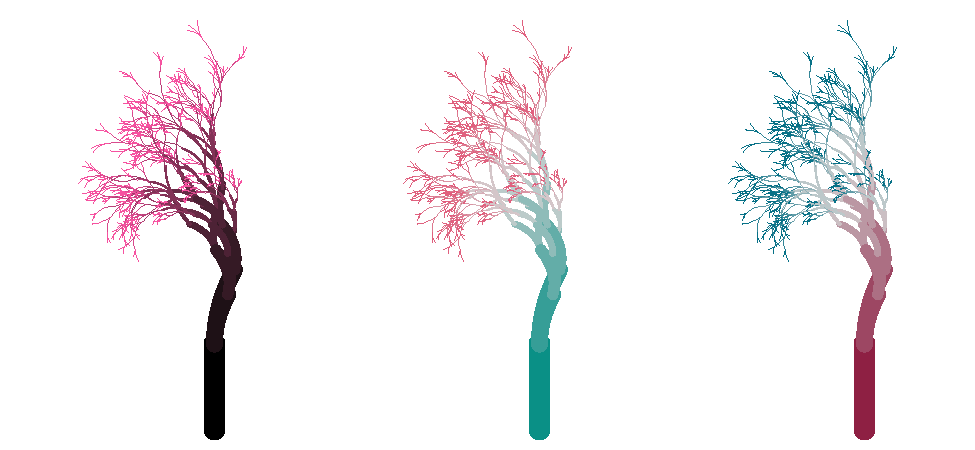
\includegraphics{_main_files/figure-latex/unnamed-chunk-45-1.pdf}

\subsection{\texorpdfstring{Data Viz has many many applications }{Data Viz has many many applications }}\label{data-viz-has-many-many-applications}

\begin{itemize}
\tightlist
\item
  Our readers/ listeners can follow us better with data viz
\item
  Statistics are much easier to understand with a visual representation
\item
  Mostly, we want to be able to \emph{see} our data ¯\textbackslash\_(ツ)\_/¯

  \begin{itemize}
  \tightlist
  \item
    Having a visual representation can be helpful in understanding relationships between variables
  \item
    Many common statistics make assumptions about the \emph{distribution} of our data, so we need to check/test that!
  \end{itemize}
\end{itemize}

\subsection{Example: Sine \& Cosine}\label{example-sine-cosine}

\begin{itemize}
\tightlist
\item
  \ldots are trigonometric angle functions with a special relationship
\item
  This relationship cannot be found with common statistics - the correlation
\end{itemize}

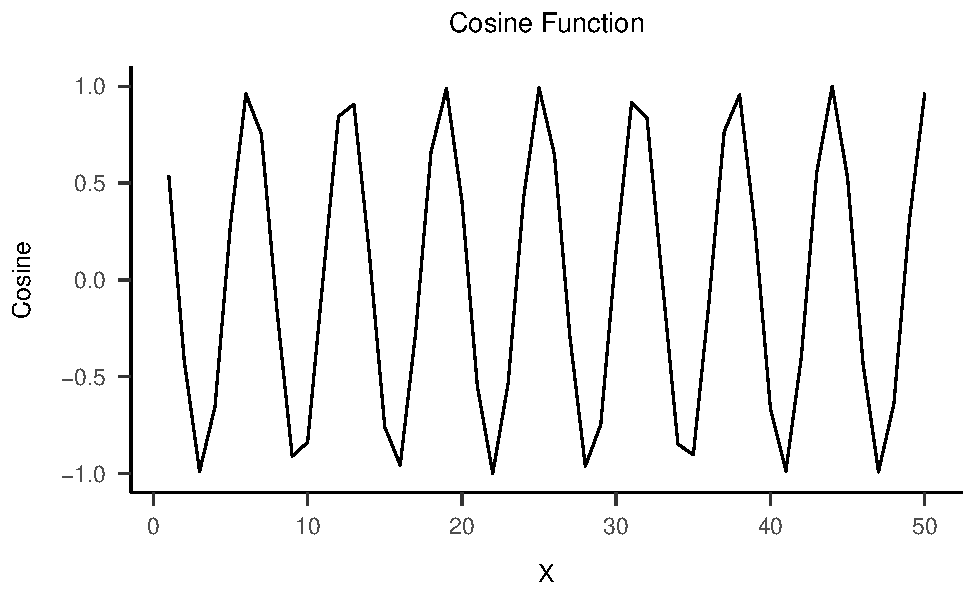
\includegraphics{_main_files/figure-latex/unnamed-chunk-46-1.pdf}

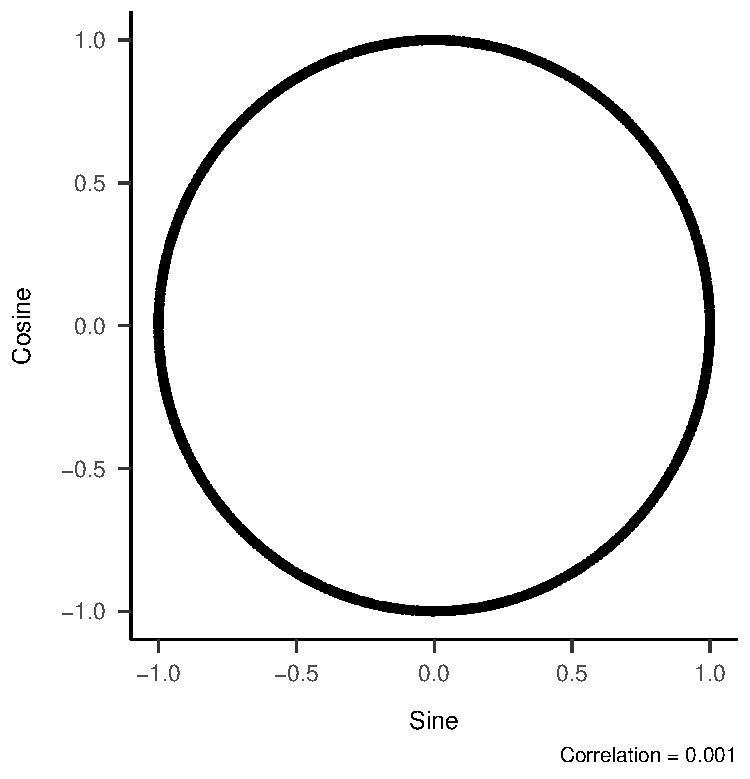
\includegraphics{_main_files/figure-latex/unnamed-chunk-47-1.pdf}

\begin{itemize}
\tightlist
\item
  Data Viz helps us not to make wrong assumptions about our data!
\end{itemize}

\section{\texorpdfstring{What is \texttt{ggplot2}?}{What is ggplot2?}}\label{what-is-ggplot2}

\begin{itemize}
\item
  Probably the best data visualization package in R
\item
  Powerful tool for visualizing data
\item
  Part of the \texttt{tidyverse} ♥
\end{itemize}

\begin{itemize}
\tightlist
\item
  \texttt{library(ggplot2)}
\end{itemize}

\subsection{\texorpdfstring{Most important \texttt{ggplot2} functions}{Most important ggplot2 functions}}\label{most-important-ggplot2-functions}

\subsubsection{\texorpdfstring{\texttt{ggplot()}}{ggplot()}}\label{ggplot}

\begin{itemize}
\tightlist
\item
  The main function for ``opening the canvas''
\item
  This function prepares R for the plot definition
\item
  Commonly, we define the data set and which variables to plot in this function
\item
  Needs the \emph{aesthetics} function \texttt{aes()} as input
\item
  It's important to remember that the package is
  called \emph{ggplot\textbf{2}} while the function call is \emph{ggplot}!
\end{itemize}

\subsection{\texorpdfstring{\texttt{geom\_XYZ()}}{geom\_XYZ()}}\label{geom_xyz}

\begin{itemize}
\tightlist
\item
  Defines the actual type of plot = \emph{geometric objects}
\item
  When data is pre-defined, this function does not \emph{need} additional input
\item
  Can handle some ``pretty makers'', such as \texttt{alpha}, which defines color opacity
\item
  \emph{geom\_bar, geom\_boxplot, geom\_density, geom\_jitter, geom\_histogram}
\end{itemize}

\section{Example: Basic Bar Plot}\label{example-basic-bar-plot}

\begin{Shaded}
\begin{Highlighting}[]
\FunctionTok{ggplot}\NormalTok{(iris) }\SpecialCharTok{+} 
  \FunctionTok{geom\_bar}\NormalTok{(}\FunctionTok{aes}\NormalTok{(}\AttributeTok{x =}\NormalTok{ Petal.Width)) }
\end{Highlighting}
\end{Shaded}

\begin{flushleft}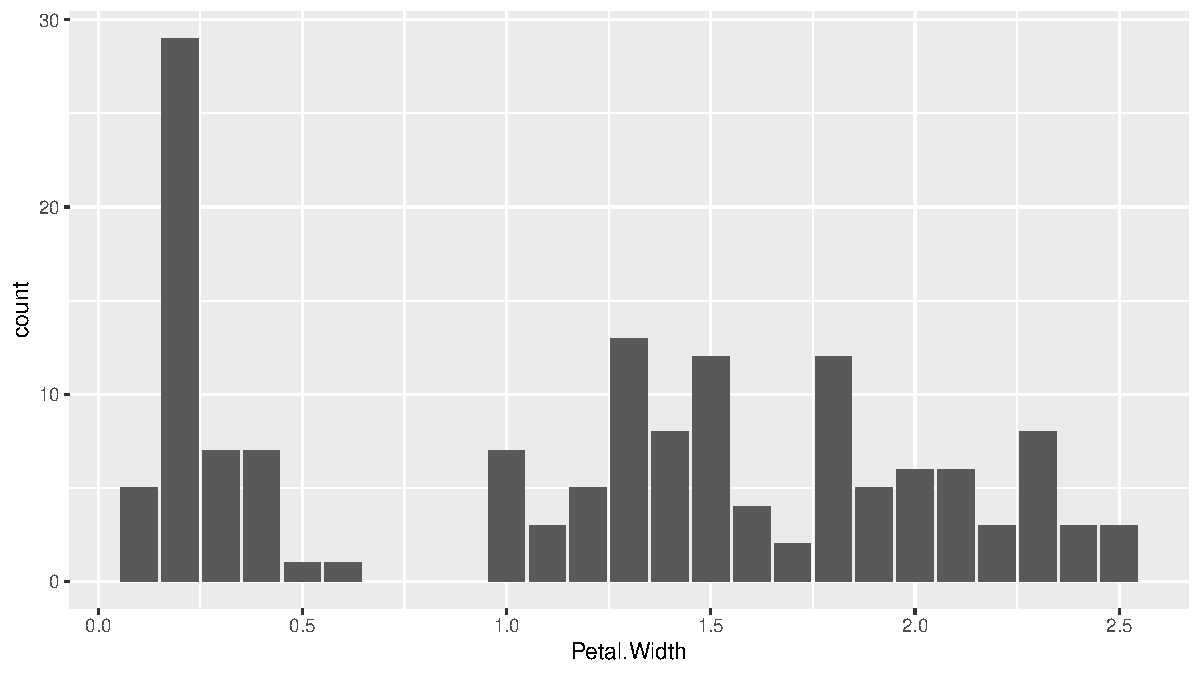
\includegraphics{_main_files/figure-latex/unnamed-chunk-48-1} \end{flushleft}

\subsection{Making Plots Prettier}\label{making-plots-prettier}

\begin{itemize}
\tightlist
\item
  color

  \begin{itemize}
  \tightlist
  \item
    visual property of the geometric object
  \item
    which color for the outlines
  \item
    \texttt{colors()}
  \end{itemize}
\item
  fill

  \begin{itemize}
  \tightlist
  \item
    visual property of the geometric object
  \item
    which color to fill
  \end{itemize}
\item
  labs
\item
  theme

  \begin{itemize}
  \tightlist
  \item
    \texttt{install.packages("papaja")} \(\rightarrow\) \texttt{library(papaja)}
  \end{itemize}
\end{itemize}

\subsection{Example: Bar Plot with color and fill}\label{example-bar-plot-with-color-and-fill}

\begin{Shaded}
\begin{Highlighting}[]
\FunctionTok{ggplot}\NormalTok{(iris) }\SpecialCharTok{+} 
  \FunctionTok{geom\_bar}\NormalTok{(}\FunctionTok{aes}\NormalTok{(}\AttributeTok{x =}\NormalTok{ Petal.Width), }\AttributeTok{color =} \StringTok{"deepskyblue3"}\NormalTok{, }\AttributeTok{fill =} \StringTok{"deepskyblue"}\NormalTok{)}
\end{Highlighting}
\end{Shaded}

\begin{flushleft}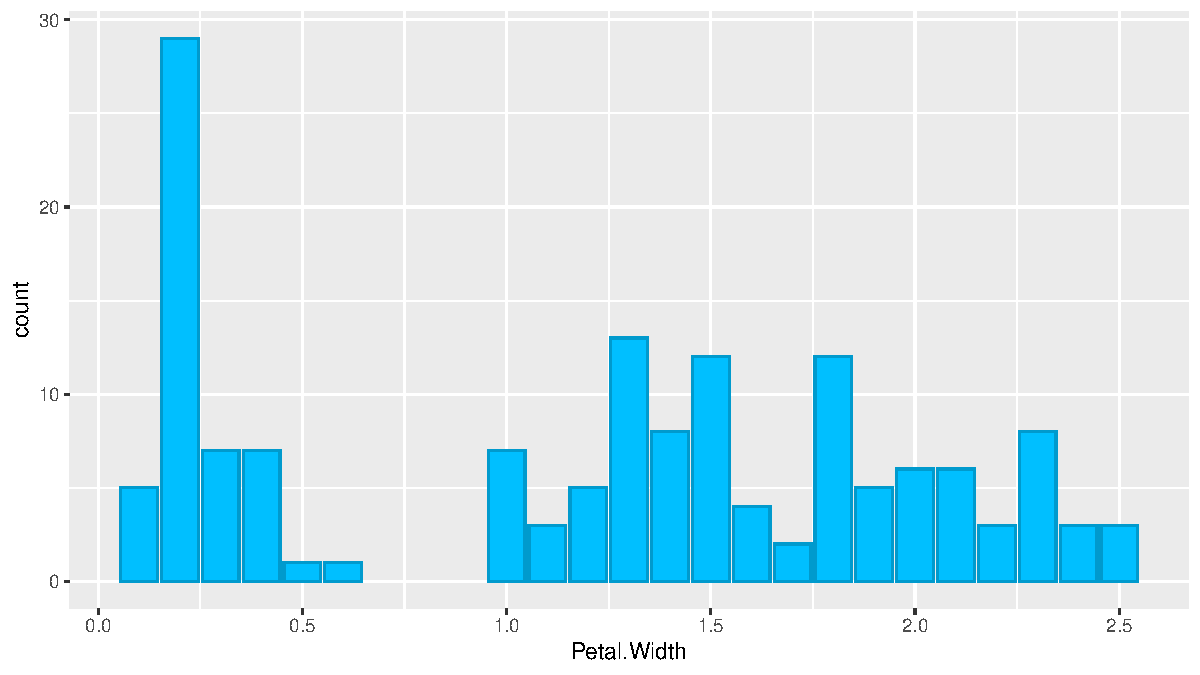
\includegraphics{_main_files/figure-latex/unnamed-chunk-49-1} \end{flushleft}

\begin{itemize}
\tightlist
\item
  What could cause this distribution?
\end{itemize}

\subsection{Example: Bar Plot with color and fill}\label{example-bar-plot-with-color-and-fill-1}

\begin{Shaded}
\begin{Highlighting}[]
\FunctionTok{ggplot}\NormalTok{(iris) }\SpecialCharTok{+} 
  \FunctionTok{geom\_bar}\NormalTok{(}\FunctionTok{aes}\NormalTok{(}\AttributeTok{x =}\NormalTok{ Petal.Width, }\AttributeTok{color =}\NormalTok{ Species, }\AttributeTok{fill =}\NormalTok{ Species))}
\end{Highlighting}
\end{Shaded}

\begin{flushleft}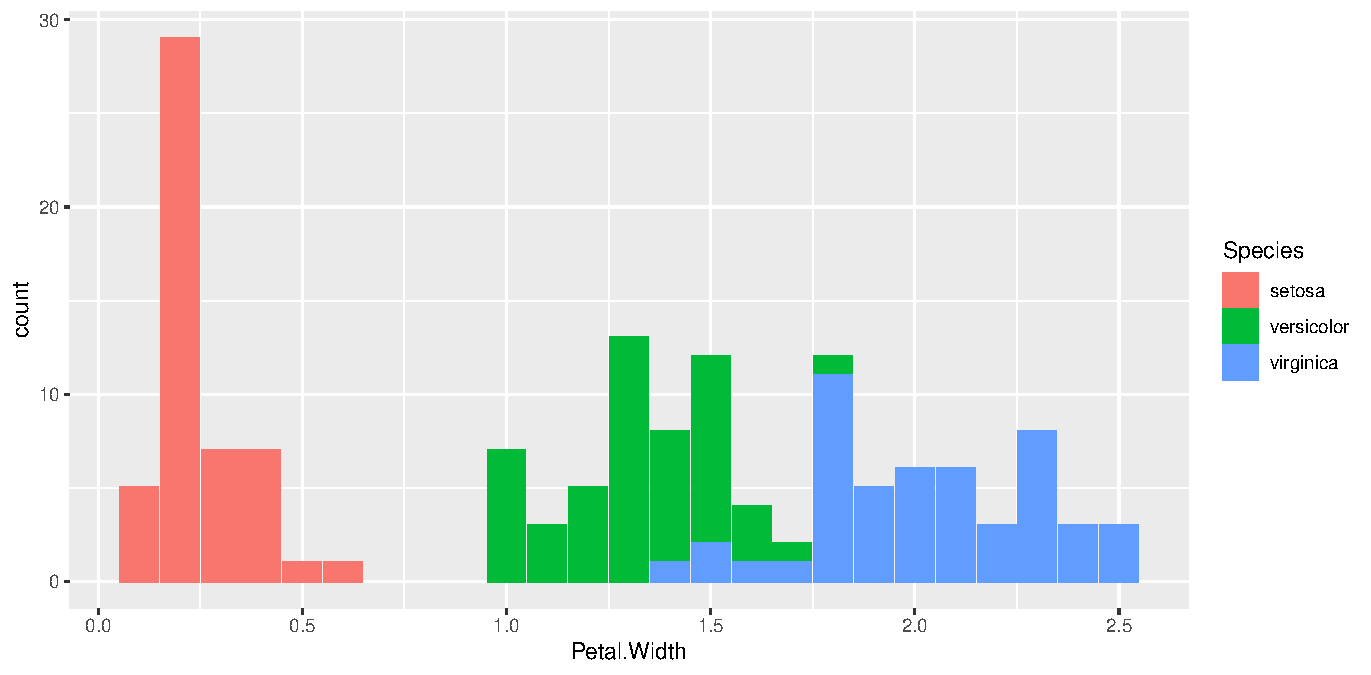
\includegraphics{_main_files/figure-latex/unnamed-chunk-50-1} \end{flushleft}

\begin{itemize}
\tightlist
\item
  What do you notice about the code compared to before?
\end{itemize}

\subsection{Static vs.~Dynamic Aesthetics}\label{static-vs.-dynamic-aesthetics}

\begin{itemize}
\tightlist
\item
  \textbf{Static Aesthetics}: Fixed values applied to all elements of the plot

  \begin{itemize}
  \tightlist
  \item
    Example: \emph{color = ``deepskyblue3''}
  \item
    Means every element will have the same color.
  \end{itemize}
\item
  \textbf{Dynamic Aesthetics}: These map a variable in your data to an aesthetic, which allows different elements to have different colors based on the data

  \begin{itemize}
  \tightlist
  \item
    Example: \emph{aes(color = Species)}
  \item
    Means the color will vary according to the Species variable in the data set.
  \end{itemize}
\end{itemize}

\subsection{Exercise}\label{exercise-5}

Create a \textbf{density plot} that shows \emph{Sepal.Length} from the \texttt{iris} data set.
\emph{Fill} in the color depending on the Species and \emph{color} the outlines with ``white''.
Make sure everything is visible and legible, so try to use an \emph{alpha} of around 0.6.

\begin{Shaded}
\begin{Highlighting}[]
\FunctionTok{ggplot}\NormalTok{(data) }\SpecialCharTok{+} 
  \FunctionTok{geom\_XYZ}\NormalTok{(}\FunctionTok{aes}\NormalTok{(), }\AttributeTok{alpha =}\NormalTok{ ?)}
\end{Highlighting}
\end{Shaded}

\subsection{Solution}\label{solution-9}

\begin{Shaded}
\begin{Highlighting}[]
\FunctionTok{ggplot}\NormalTok{(iris) }\SpecialCharTok{+} 
  \FunctionTok{geom\_density}\NormalTok{(}\FunctionTok{aes}\NormalTok{(}\AttributeTok{x =}\NormalTok{ Sepal.Length, }\AttributeTok{fill =}\NormalTok{ Species), }
               \AttributeTok{color =} \StringTok{"white"}\NormalTok{, }\AttributeTok{alpha =}\NormalTok{ .}\DecValTok{6}\NormalTok{)}
\end{Highlighting}
\end{Shaded}

\begin{flushleft}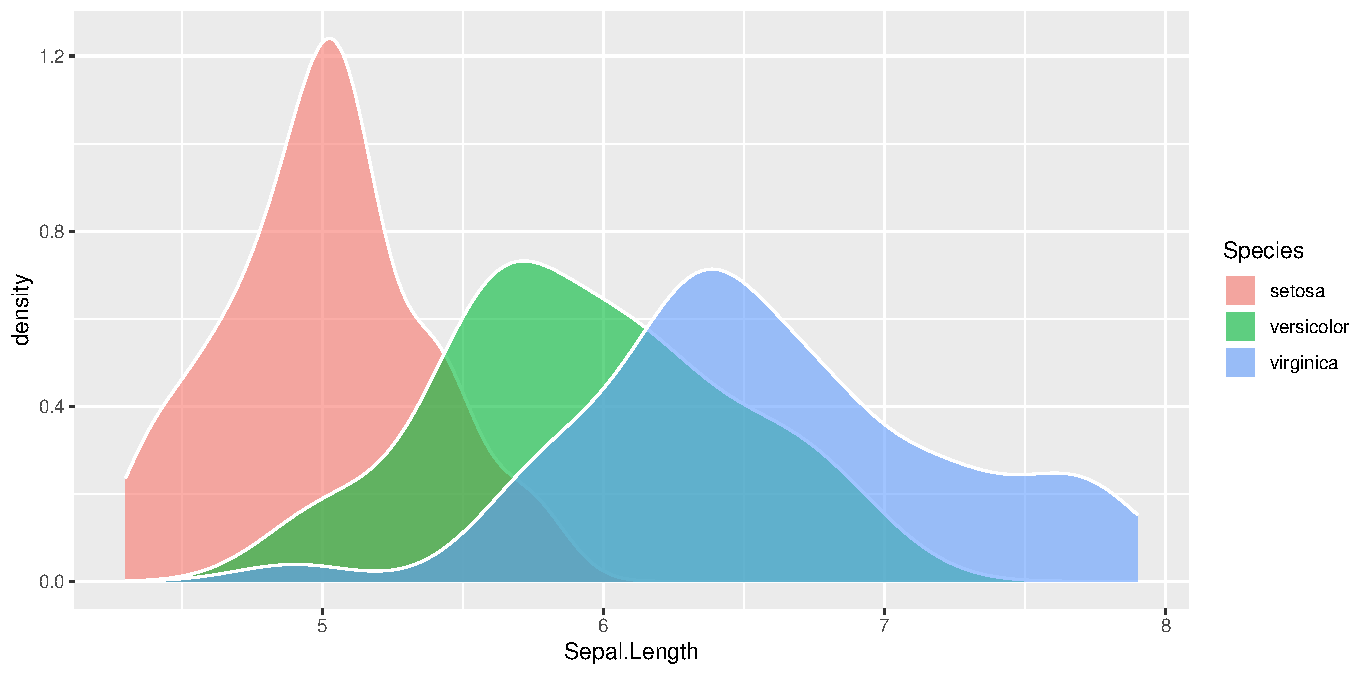
\includegraphics{_main_files/figure-latex/unnamed-chunk-52-1} \end{flushleft}

\section{Adding labels and themes}\label{adding-labels-and-themes}

\begin{itemize}
\tightlist
\item
  A good plot should be self explanatory and clear
\item
  We need labels to tell others what our plot shows

  \begin{itemize}
  \tightlist
  \item
    Especially when using color for another variable, it needs to be clear what each color means
  \end{itemize}
\item
  Also the gray-ish default background is ok, but neither very pretty nor very clear

  \begin{itemize}
  \tightlist
  \item
    It is sometimes advisable to keep grid lines visible, but sometimes they can be distracting and unnecessary
  \item
    ggplot2 has a lot of built-in theme options, but there are many packages that provide their own themes
  \item
    Usually \emph{my preference} is \texttt{papaja::theme\_apa()}, which adheres to APA guidelines
  \end{itemize}
\end{itemize}

\subsection{Same example with added theme}\label{same-example-with-added-theme}

\begin{Shaded}
\begin{Highlighting}[]
\FunctionTok{ggplot}\NormalTok{(iris) }\SpecialCharTok{+} 
  \FunctionTok{geom\_bar}\NormalTok{(}\FunctionTok{aes}\NormalTok{(}\AttributeTok{x =}\NormalTok{ Petal.Width, }\AttributeTok{color =}\NormalTok{ Species, }\AttributeTok{fill =}\NormalTok{ Species)) }\SpecialCharTok{+}
  \FunctionTok{theme\_apa}\NormalTok{()}
\end{Highlighting}
\end{Shaded}

\begin{flushleft}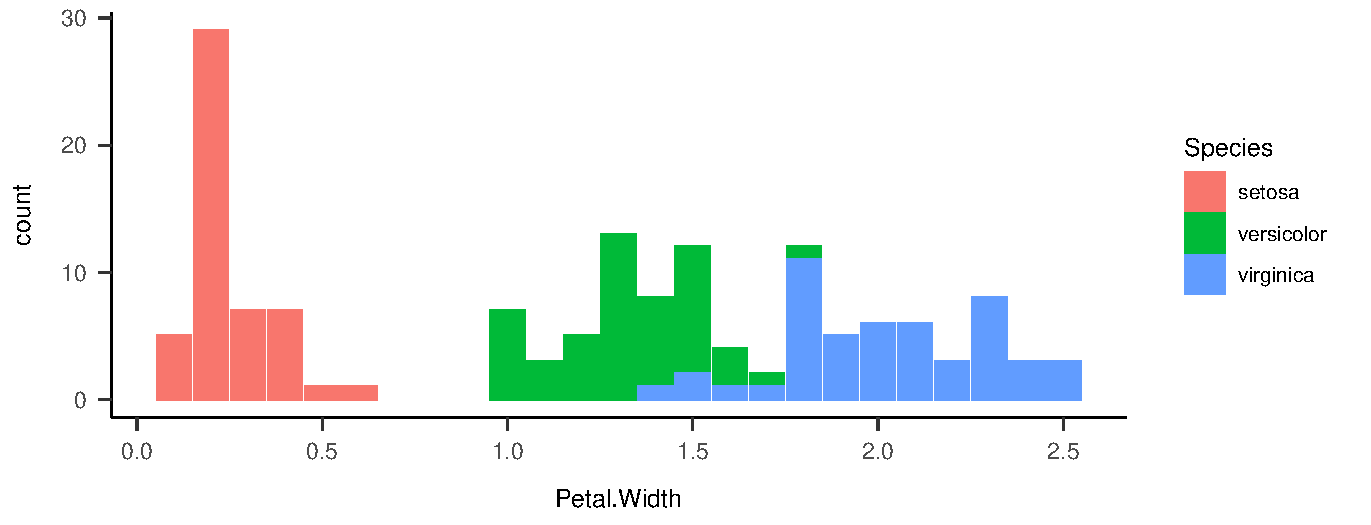
\includegraphics{_main_files/figure-latex/unnamed-chunk-53-1} \end{flushleft}

\begin{itemize}
\tightlist
\item
  What labels should we use in this plot?
\end{itemize}

\subsection{Same example with added theme and labels}\label{same-example-with-added-theme-and-labels}

\begin{Shaded}
\begin{Highlighting}[]
\FunctionTok{ggplot}\NormalTok{(iris) }\SpecialCharTok{+} 
  \FunctionTok{geom\_bar}\NormalTok{(}\FunctionTok{aes}\NormalTok{(}\AttributeTok{x =}\NormalTok{ Petal.Width, }\AttributeTok{color =}\NormalTok{ Species, }\AttributeTok{fill =}\NormalTok{ Species)) }\SpecialCharTok{+}
  \FunctionTok{theme\_apa}\NormalTok{() }\SpecialCharTok{+}
  \FunctionTok{labs}\NormalTok{(}\AttributeTok{x =} \StringTok{"Petal Width"}\NormalTok{, }\AttributeTok{y =} \StringTok{"Flower Count"}\NormalTok{,}
       \AttributeTok{title =} \StringTok{"Size of Iris Flowers"}\NormalTok{)}
\end{Highlighting}
\end{Shaded}

\begin{flushleft}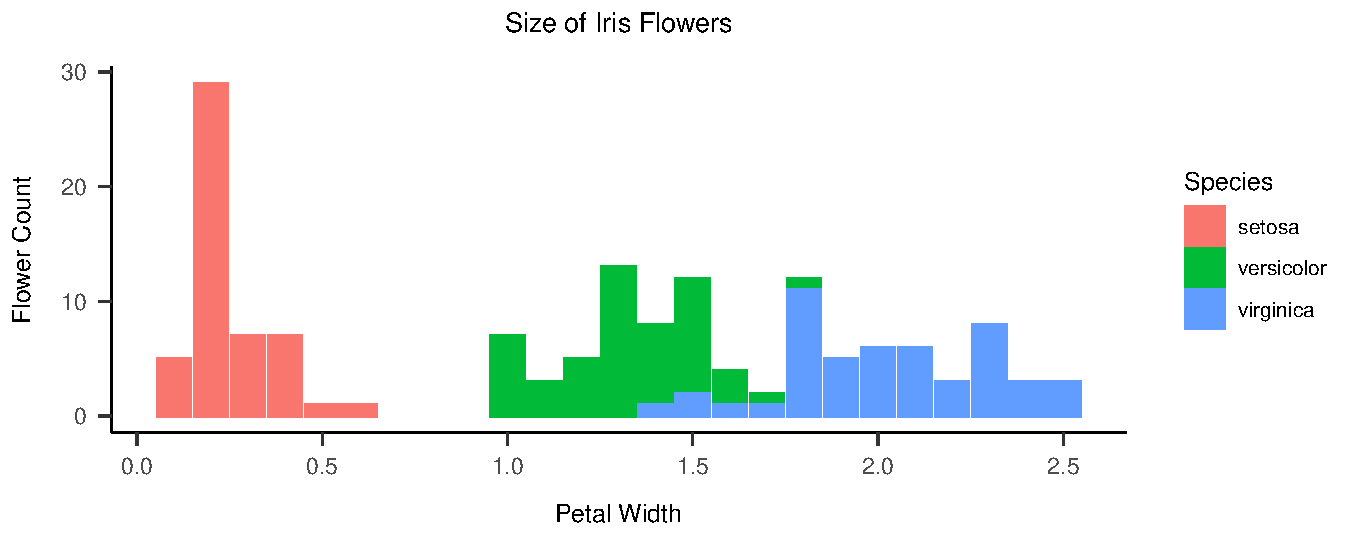
\includegraphics{_main_files/figure-latex/unnamed-chunk-54-1} \end{flushleft}

\section{Bivariate Visualizations}\label{bivariate-visualizations}

\begin{itemize}
\tightlist
\item
  The bar plot shows the distribution of a single variable

  \begin{itemize}
  \tightlist
  \item
    We can add color to show groups
  \end{itemize}
\item
  Showing the relationship of two variables to each other is crucial for understanding our data

  \begin{itemize}
  \tightlist
  \item
    We can still add color to make existing groups clearer or add a third variable
  \end{itemize}
\item
  For a broad overview of which visualization (and statistic) to use for which type of data, visit the \href{https://the-tave.shinyapps.io/Statistics-Picker/}{Statistics Picker} (currently only available in German)

  \begin{itemize}
  \tightlist
  \item
    Most common are boxplots, scatterplots \& line graphs
  \end{itemize}
\end{itemize}

\subsection{Boxplot Example}\label{boxplot-example}

As suggested by one of you, we will look at the relationship of preferred music genre and music volume in our course:

\begin{Shaded}
\begin{Highlighting}[]
\CommentTok{\# seminar \textless{}{-} readRDS("./data/seminar\_data.Rds")}
\FunctionTok{ggplot}\NormalTok{(seminar, }\FunctionTok{aes}\NormalTok{(}\AttributeTok{x=}\NormalTok{v07\_genre, }\AttributeTok{y=}\NormalTok{v08\_loudness, }\AttributeTok{colour=}\NormalTok{v07\_genre, }\AttributeTok{fill=}\NormalTok{v07\_genre)) }\SpecialCharTok{+}
  \FunctionTok{geom\_boxplot}\NormalTok{(}\AttributeTok{alpha =} \FloatTok{0.7}\NormalTok{) }\SpecialCharTok{+} \FunctionTok{theme\_apa}\NormalTok{() }\SpecialCharTok{+}
  \FunctionTok{labs}\NormalTok{(}\AttributeTok{x =} \StringTok{"Preferred Music Genre"}\NormalTok{, }\AttributeTok{y =} \StringTok{"Loudness (arbitrary units)"}\NormalTok{, }
       \AttributeTok{color =} \StringTok{"Genre"}\NormalTok{, }\AttributeTok{fill =} \StringTok{"Genre"}\NormalTok{)}
\end{Highlighting}
\end{Shaded}

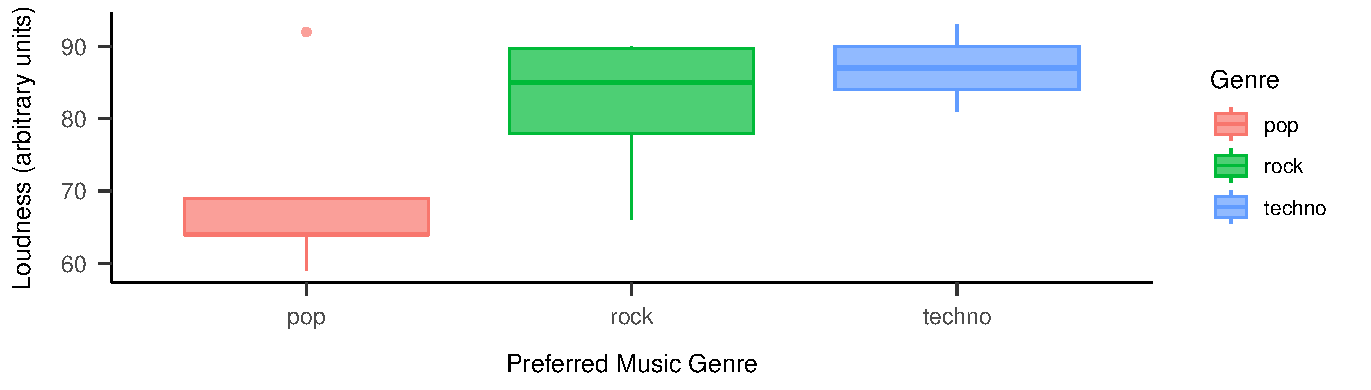
\includegraphics{_main_files/figure-latex/unnamed-chunk-55-1.pdf}

\subsection{Exercise: Boxplot}\label{exercise-boxplot}

Create a \textbf{box plot} that shows \emph{Sepal.Length} from the \texttt{iris} data set grouped by the \emph{Species}.
\emph{Fill} and \emph{color} depending on the Species.
Make sure everything is visible and legible, so try to use an \emph{alpha} of around 0.7.
Try to add \emph{labels} and a \emph{theme}.

\subsection{Solution: Boxplot}\label{solution-boxplot}

\begin{Shaded}
\begin{Highlighting}[]
\FunctionTok{ggplot}\NormalTok{(iris) }\SpecialCharTok{+} 
  \FunctionTok{geom\_boxplot}\NormalTok{(}\FunctionTok{aes}\NormalTok{(}\AttributeTok{x =}\NormalTok{ Species, }\AttributeTok{y =}\NormalTok{ Sepal.Length,}
                   \AttributeTok{color =}\NormalTok{ Species, }\AttributeTok{fill =}\NormalTok{ Species), }\AttributeTok{alpha =}\NormalTok{ .}\DecValTok{6}\NormalTok{) }\SpecialCharTok{+}
  \FunctionTok{theme\_minimal}\NormalTok{() }\SpecialCharTok{+} \FunctionTok{labs}\NormalTok{(}\AttributeTok{x =} \StringTok{"Species"}\NormalTok{, }\AttributeTok{y =} \StringTok{"Sepal Length"}\NormalTok{)}
\end{Highlighting}
\end{Shaded}

\begin{flushleft}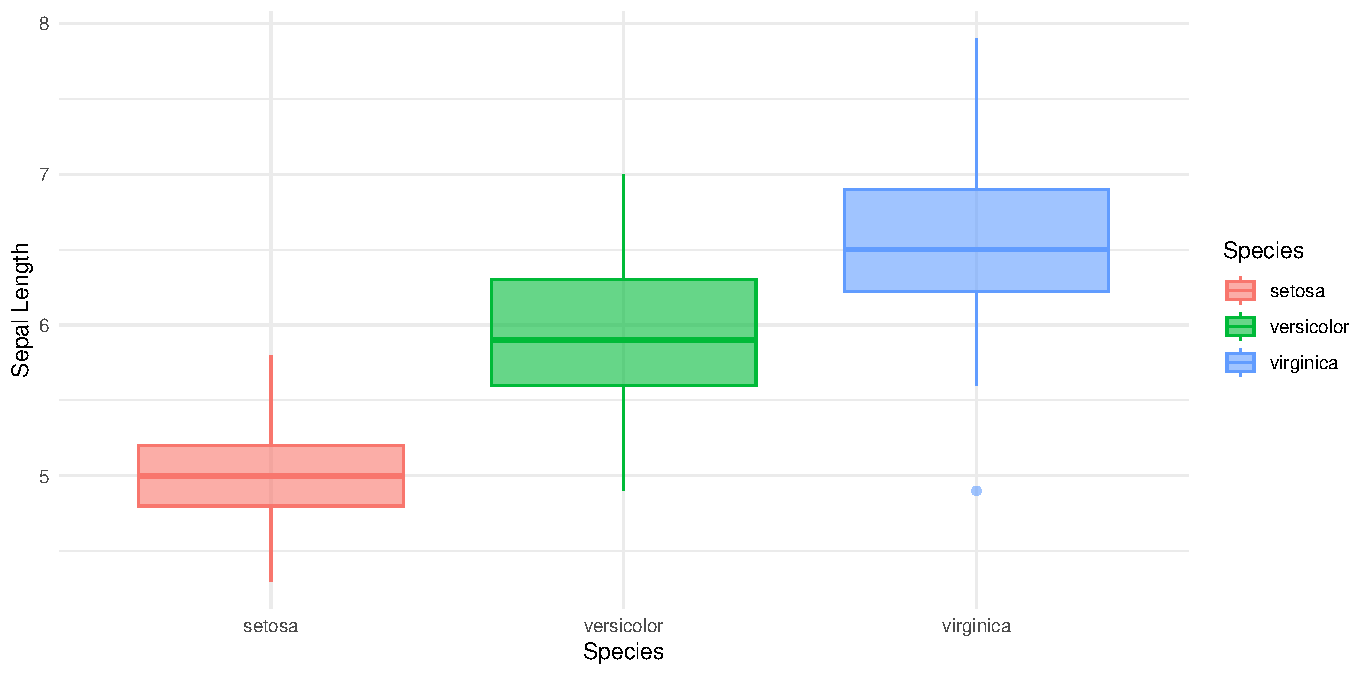
\includegraphics{_main_files/figure-latex/unnamed-chunk-56-1} \end{flushleft}

\subsection{Inspiration: colors and palettes}\label{inspiration-colors-and-palettes}

\begin{itemize}
\tightlist
\item
  These plots have all used the default colors from ggplot2
\item
  There are many options for customization, either:

  \begin{itemize}
  \tightlist
  \item
    Use the ``brewer'' palettes from \texttt{ggplot2} with \texttt{scale\_color\_brewer()} or \texttt{scale\_fill\_brewer()}
  \item
    Choose single colors (static aesthetics), check \texttt{colors()} for R color names
  \item
    Create a color palette with all colors that you need and use it with \texttt{scale\_color\_manual()} or \texttt{scale\_fill\_manual()}
  \item
    Use a predefined color palette from packages like \texttt{viridis} or \texttt{unikn} or \texttt{RColorBrewer}\ldots{}
  \end{itemize}
\item
  Have fun with it!
\end{itemize}

\subsection{Use: colors and palettes}\label{use-colors-and-palettes}

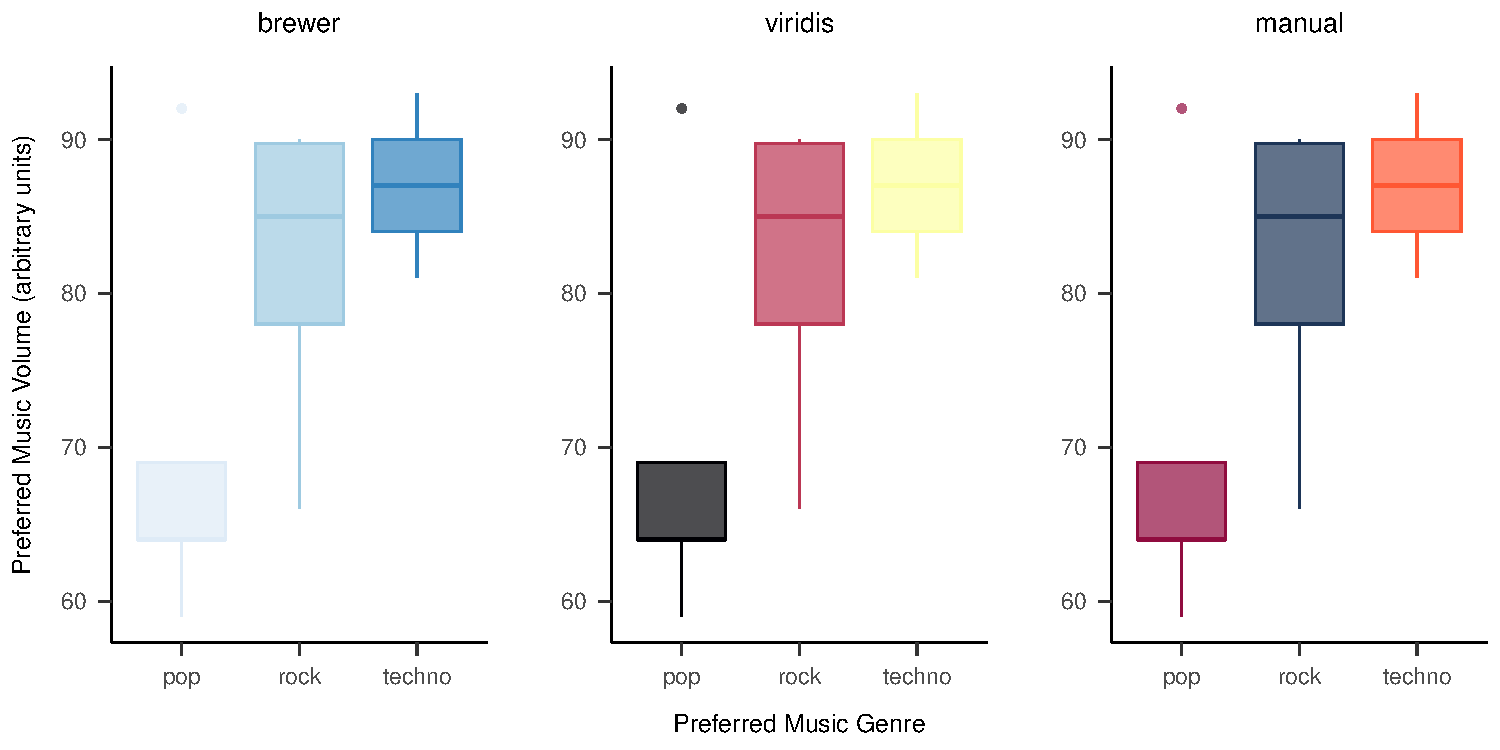
\includegraphics{_main_files/figure-latex/unnamed-chunk-57-1.pdf}

\begin{itemize}
\tightlist
\item
  Showing plots together like this is easy with \texttt{cowplot::plot\_grid()}!
\end{itemize}

\section{Wrap-Up \& Further Resources}\label{wrap-up-further-resources-5}

\texttt{ggplot2} is a powerful tool for visualizing data

Plot commands are added together with + and executed as one

A basic plot is created with ggplot() + geom\_XYZ(), e.g.~geom\_bar

color \& fill give you nice color options (static \& dynamic)

labs() adds labels to the plot (i.e.~x, y, title, \ldots)

Themes control the background of the plot, e.g.~papaja::theme\_apa() or theme\_minimal()

Color palettes are a great way of elevating a visualization

\href{https://ggplot2.tidyverse.org/articles/ggplot2.html}{ggplot2 vignette}

\href{https://r-graphics.org/}{R Graphics Cookbook}

\href{https://hneth.github.io/unikn/index.html}{unikn}

\href{https://sjmgarnier.github.io/viridisLite/reference/viridis.html}{viridis}

\href{https://www.rdocumentation.org/packages/papaja/versions/0.1.2}{papaja}

\href{https://www.cedricscherer.com/2019/08/05/a-ggplot2-tutorial-for-beautiful-plotting-in-r/}{Beautiful Plotting Guide} Very extensive, I still profit from this guide a lot :)

\href{http://www.sthda.com/english/wiki/ggplot2-colors-how-to-change-colors-automatically-and-manually}{More color palettes explained}

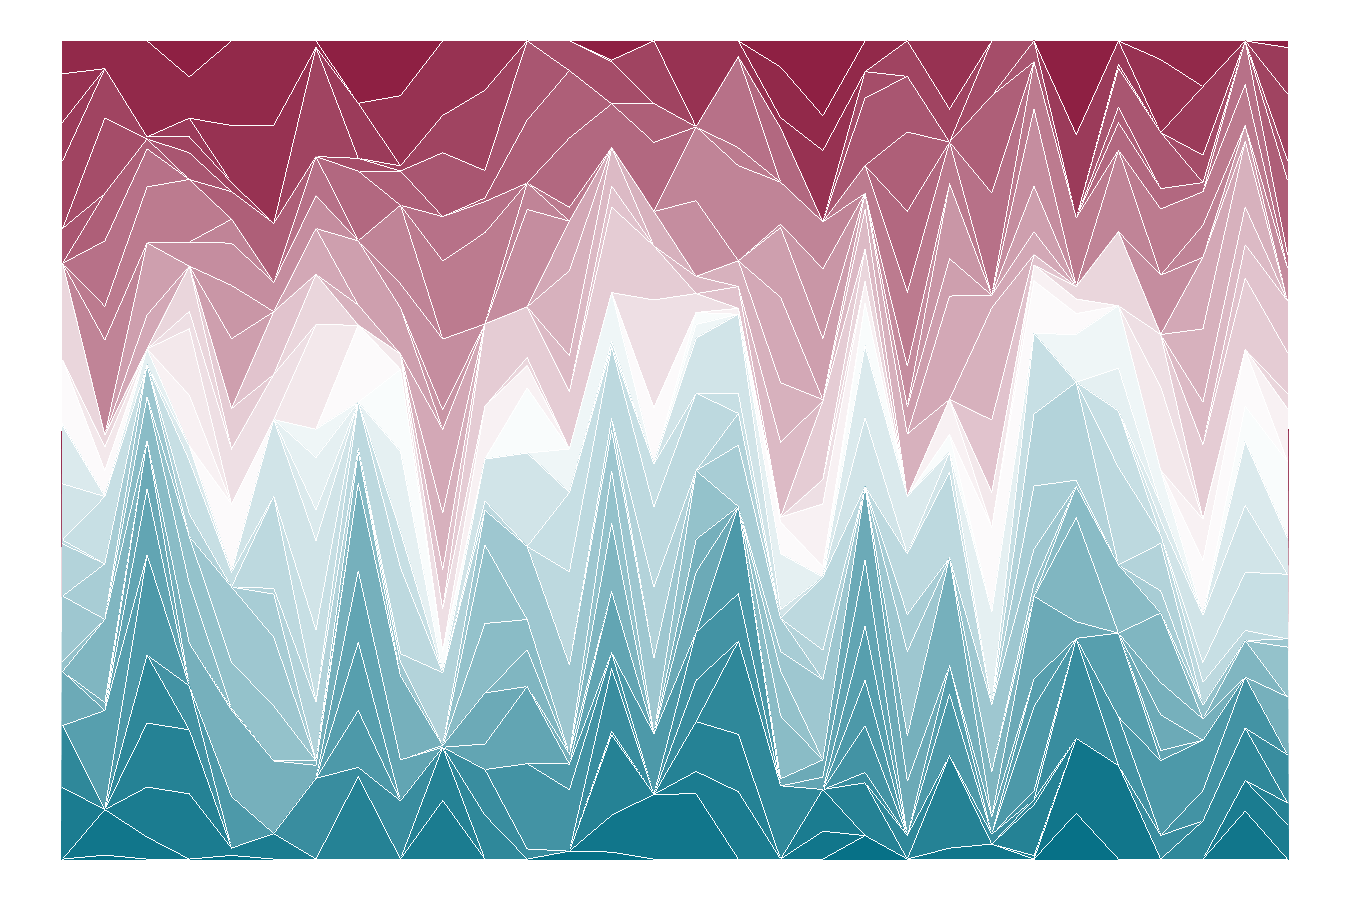
\includegraphics{_main_files/figure-latex/unikn-plot-1.pdf}

\chapter{\texorpdfstring{Creating and interpreting statistics: Chi\(^2\) \& t-test \& ANOVA}{Creating and interpreting statistics: Chi\^{}2 \& t-test \& ANOVA}}\label{creating-and-interpreting-statistics-chi2-t-test-anova}

\begin{itemize}
\tightlist
\item
  Re-cap of statistics: t-test, Chi\(^2\) and ANOVA
\item
  Learn how to calculate in R
\item
  Learn how to check assumptions
\item
  Go over examples (inspired by your thesis analyses )
\end{itemize}

\section{\texorpdfstring{Statistics Re-cap I}{Statistics Re-cap  I}}\label{statistics-re-cap-i}

What do you remember from statistics:

\begin{itemize}
\tightlist
\item
  What is Chi\(^2\) / \(\chi^2\)?
\item
  What is the t-test?
\item
  What is an ANOVA?
\item
  What do they have in common \& what differentiates them?
\end{itemize}

\subsection{\texorpdfstring{Statistics Re-cap II}{Statistics Re-cap  II}}\label{statistics-re-cap-ii}

They measure \emph{group differences}

\begin{itemize}
\tightlist
\item
  \(\chi^2\) \(\rightarrow\) nominal data
\item
  t-Test \(\rightarrow\) one or two \emph{groups} with a continuous attribute
\item
  ANOVA \(\rightarrow\) three or more groups with one (or more) continuous attribute(s)
\end{itemize}

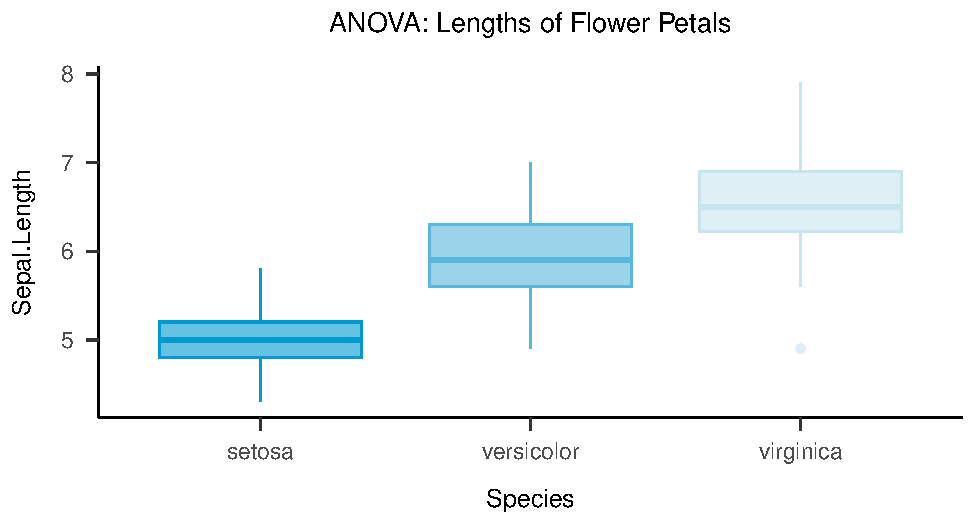
\includegraphics{_main_files/figure-latex/unnamed-chunk-60-1.pdf}

\subsection{Pre-Requisites}\label{pre-requisites}

\begin{itemize}
\tightlist
\item
  Load the seminar data using \texttt{seminar\ \textless{}-\ readRDS("./data/seminar\_data.Rds")}

  \begin{itemize}
  \tightlist
  \item
    Please make sure you are using the R dataset from the
    zip folder in ILIAS, not the original csv file we first used!
  \end{itemize}
\item
  Add a ``dummy variable'' (only two possible values 0 and 1)
  for believing in a soul, where 1 means \emph{yes} and 0 means \emph{no or unsure}

  \begin{itemize}
  \tightlist
  \item
    \texttt{seminar\$soul\_dummy\ \textless{}-}
    \texttt{ifelse(seminar\$v11\_soul\ ==\ "yes",\ 1,\ 0)}
  \end{itemize}
\end{itemize}

\section{\texorpdfstring{\(\chi^2\)}{\textbackslash chi\^{}2}}\label{chi2}

\begin{itemize}
\tightlist
\item
  \(\chi^2\) Test for Independence: Determines if there is an association between \textbf{two categorical variables} in a contingency table

  \begin{itemize}
  \tightlist
  \item
    compares the observed frequencies in each category of a contingency table to the frequencies expected if the variables were independent
  \end{itemize}
\end{itemize}

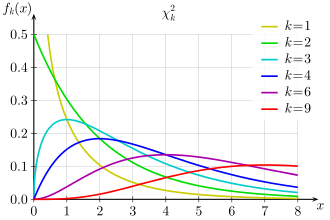
\includegraphics{./img/chidist.png}k

\subsection{Calculation:}\label{calculation}

\begin{itemize}
\item
  \[\chi^2 = \sum \frac{(O_i - E_i)^2}{E_i}\]
\item
  \(O_i\) is the observed frequency in each category
\item
  \(E_i\) is the expected frequency in each category, calculated as: \[E_i = \frac{(row \ total) \times (column \ total)}{grand \ total}\]
\item
  Example: Believing in the soul by gender
\item
\begin{verbatim}
##        
##          0  1 Sum
##   man    1  1   2
##   woman  6  5  11
##   Sum    7  6  13
\end{verbatim}
\end{itemize}

\subsection{How to in R}\label{how-to-in-r}

\begin{itemize}
\item
  The \texttt{chisq.test()} function only needs (categorical!) \emph{x, y} as input

  \begin{itemize}
  \tightlist
  \item
    Especially with a small sample, we can add the parameter \emph{simulate.p.value = T}, which bootstraps the analysis 2000 times
  \end{itemize}
\item
\begin{Shaded}
\begin{Highlighting}[]
\FunctionTok{chisq.test}\NormalTok{(seminar}\SpecialCharTok{$}\NormalTok{v01\_gender, seminar}\SpecialCharTok{$}\NormalTok{soul\_dummy, }\AttributeTok{simulate.p.value =}\NormalTok{ T)}
\end{Highlighting}
\end{Shaded}

\begin{verbatim}
## 
##    Pearson's Chi-squared test with simulated p-value (based on 2000
##    replicates)
## 
## data:  seminar$v01_gender and seminar$soul_dummy
## X-squared = 0.014069, df = NA, p-value = 1
\end{verbatim}
\end{itemize}

\subsection{\texorpdfstring{Exercise }{Exercise  }}\label{exercise-6}

We want to explore whether \textbf{belief in the soul (dummy)} is associated with \textbf{music preference}.

Calculate a simple chisq.test and interpret the results.

\subsection{\texorpdfstring{Solution }{Solution  }}\label{solution-10}

\begin{Shaded}
\begin{Highlighting}[]
\FunctionTok{chisq.test}\NormalTok{(seminar}\SpecialCharTok{$}\NormalTok{v07\_genre, seminar}\SpecialCharTok{$}\NormalTok{soul\_dummy)}
\end{Highlighting}
\end{Shaded}

\begin{verbatim}
## Warning in chisq.test(seminar$v07_genre, seminar$soul_dummy): Chi-squared
## approximation may be incorrect
\end{verbatim}

\begin{verbatim}
## 
##  Pearson's Chi-squared test
## 
## data:  seminar$v07_genre and seminar$soul_dummy
## X-squared = 2.1357, df = 2, p-value = 0.3437
\end{verbatim}

\begin{Shaded}
\begin{Highlighting}[]
\FunctionTok{addmargins}\NormalTok{(}\FunctionTok{table}\NormalTok{(seminar}\SpecialCharTok{$}\NormalTok{v07\_genre, seminar}\SpecialCharTok{$}\NormalTok{soul\_dummy))}
\end{Highlighting}
\end{Shaded}

\begin{verbatim}
##         
##           0  1 Sum
##   pop     2  3   5
##   rock    3  3   6
##   techno  2  0   2
##   Sum     7  6  13
\end{verbatim}

\begin{itemize}
\tightlist
\item
  Interpretation?
\end{itemize}

\section{t-Test}\label{t-test}

\begin{itemize}
\item
  There are 3 broad categories of t-test:
\item
  \textbf{one-sample} t-test:

  \begin{itemize}
  \tightlist
  \item
    Test one sample against a known mean value
  \end{itemize}
\item
  \textbf{two-sample} t-test (independent):

  \begin{itemize}
  \tightlist
  \item
    Test two sample-means against each other (independent samples)
  \end{itemize}
\item
  \textbf{paired two-sample} t-test:

  \begin{itemize}
  \tightlist
  \item
    Test two dependent sample-means against each other (e.g.~repeated measures)
  \end{itemize}
\end{itemize}

\subsection{\texorpdfstring{Test statistic \emph{t}}{Test statistic t}}\label{test-statistic-t}

\begin{itemize}
\tightlist
\item
  Test statistic T has a known distribution that depends on the \textbf{degrees of freedom}, calculated as n-1
\item
  Most (probable) T values are around 0

  \begin{itemize}
  \tightlist
  \item
    The further away the T value is from 0, the less likely it is caused by chance alone \(\rightarrow\) \emph{significance}
  \end{itemize}
\end{itemize}

\begin{figure}
\centering
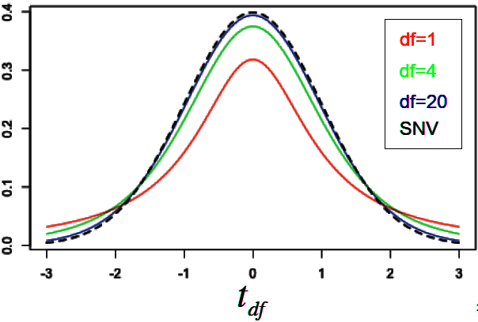
\includegraphics{./img/tdist.png}
\caption{T distribution}
\end{figure}

\subsection{\texorpdfstring{Test statistic \emph{t}}{Test statistic t}}\label{test-statistic-t-1}

\begin{itemize}
\item
  One sample: \[ t = \frac{\bar{X} - \mu}{\frac{s}{\sqrt{n}}} \]
\item
  Two sample: \[t = \frac{\bar{X}_1 - \bar{X}_2}{\sqrt{\frac{s_1^2}{n_1} + \frac{s_2^2}{n_2}}} \]
\end{itemize}

\subsection{How to in R}\label{how-to-in-r-1}

\begin{itemize}
\tightlist
\item
  The basic function is \texttt{t.test()} for any type of t.test
\item
  One sample needs inputs \emph{x, mu} (if x is from a data set you should specify \emph{data})
\item
  Two sample needs either

  \begin{itemize}
  \tightlist
  \item
    \emph{x, y} (if from data set, \emph{data}) or
  \item
    \emph{x \textasciitilde{} group} (if from data set, \emph{data})
  \end{itemize}
\item
  Paired test needs \emph{paired = T}
\item
  One-sided test needs \emph{alternative = `greater'} (assumes first group mean to be larger than second; otherwise ``less'')
\end{itemize}

\subsection{Examples}\label{examples}

\begin{Shaded}
\begin{Highlighting}[]
\CommentTok{\# One sided {-} "greater" assumes that mean(x) is larger than mean(y)}
\FunctionTok{t.test}\NormalTok{(}\AttributeTok{x =} \DecValTok{10}\SpecialCharTok{:}\DecValTok{20}\NormalTok{, }\AttributeTok{y =} \DecValTok{0}\SpecialCharTok{:}\DecValTok{10}\NormalTok{, }\AttributeTok{alternative =} \StringTok{"greater"}\NormalTok{)}
\end{Highlighting}
\end{Shaded}

\begin{verbatim}
## 
##  Welch Two Sample t-test
## 
## data:  10:20 and 0:10
## t = 7.0711, df = 20, p-value = 3.713e-07
## alternative hypothesis: true difference in means is greater than 0
## 95 percent confidence interval:
##  7.56088     Inf
## sample estimates:
## mean of x mean of y 
##        15         5
\end{verbatim}

\begin{Shaded}
\begin{Highlighting}[]
\CommentTok{\# Two sided using formula \textasciitilde{} Does seminar motivation differ}
\CommentTok{\# depending on the soul{-}belief of students?}
\FunctionTok{t.test}\NormalTok{(v10\_motivation }\SpecialCharTok{\textasciitilde{}}\NormalTok{ soul\_dummy, }\AttributeTok{data =}\NormalTok{ seminar)}
\end{Highlighting}
\end{Shaded}

\begin{verbatim}
## 
##  Welch Two Sample t-test
## 
## data:  v10_motivation by soul_dummy
## t = 0.1625, df = 6.833, p-value = 0.8756
## alternative hypothesis: true difference in means between group 0 and group 1 is not equal to 0
## 95 percent confidence interval:
##  -31.14063  35.71206
## sample estimates:
## mean in group 0 mean in group 1 
##        68.28571        66.00000
\end{verbatim}

\subsection{\texorpdfstring{Exercise }{Exercise }}\label{exercise-7}

We want to test whether the \textbf{gender} stereotype that men are \textbf{more skilled with technology} appears in our seminar sample.

Perform a one-sided two-sample t-test and interpret the results.

Hint: The grouping variable ``v01\_gender'' is sorted alphabetically - so choose the ``alternative'' accordingly!

\subsection{\texorpdfstring{Solution }{Solution }}\label{solution-11}

\begin{Shaded}
\begin{Highlighting}[]
\FunctionTok{t.test}\NormalTok{(v05\_skill\_tech }\SpecialCharTok{\textasciitilde{}}\NormalTok{ v01\_gender, }\AttributeTok{data =}\NormalTok{ seminar, }\AttributeTok{alternative =} \StringTok{"greater"}\NormalTok{)}
\end{Highlighting}
\end{Shaded}

\begin{verbatim}
## 
##  Welch Two Sample t-test
## 
## data:  v05_skill_tech by v01_gender
## t = 0.38715, df = 1.2774, p-value = 0.3766
## alternative hypothesis: true difference in means between group man and group woman is greater than 0
## 95 percent confidence interval:
##  -109.5565       Inf
## sample estimates:
##   mean in group man mean in group woman 
##                46.5                36.0
\end{verbatim}

\begin{itemize}
\tightlist
\item
  Interpretation?

  \begin{itemize}
  \tightlist
  \item
    There are no significant gender differences in technological skill.
  \end{itemize}
\end{itemize}

\section{ANOVA}\label{anova}

\begin{figure}
\centering
\includesvg{./img/anova.svg}
\caption{ANOVA principle}
\end{figure}

\begin{itemize}
\tightlist
\item
  Like a t-test for more than two groups
\item
  Why do we not just calculate several t-tests?

  \begin{itemize}
  \tightlist
  \item
    \(\alpha\) inflation!
  \item
    Significance level of 0.05 means that 1/20 tests will be significant by pure chance, so more tests makes it more likely that we hit that chance and make an alpha error (falsely reject null hypothesis)
  \end{itemize}
\end{itemize}

\subsection{How to - theoretically}\label{how-to---theoretically}

\begin{enumerate}
\def\labelenumi{\arabic{enumi}.}
\tightlist
\item
  Check Assumptions

  \begin{itemize}
  \tightlist
  \item
    Data should be normally distribution \& variance in groups should be similar (homogeneous)
  \end{itemize}
\item
  Sum of Squares: Sum of Squares total, within \& between (\emph{R does this for us})

  \begin{itemize}
  \tightlist
  \item
    F-fraction as the measure of variance explained by the grouping variable in comparison to other variability in the dependent variable
  \end{itemize}
\item
  Interpretation and post-hoc tests

  \begin{itemize}
  \tightlist
  \item
    If there are any significant differences at all, we can use pairwise t-tests (with alpha correction!)
  \end{itemize}
\end{enumerate}

\subsection{\texorpdfstring{Example: Music genre and loudness }{Example: Music genre and loudness }}\label{example-music-genre-and-loudness}

\subsubsection{1. Check assumptions}\label{check-assumptions}

\begin{itemize}
\item
  Check for Homogeneity of Variance with the Levene Test
\item
\begin{Shaded}
\begin{Highlighting}[]
\CommentTok{\# Make sure the package "car" is installed first! If not, install.packages("car")}
\CommentTok{\# as.factor() forces R to recognize our group as such!}
\NormalTok{car}\SpecialCharTok{::}\FunctionTok{leveneTest}\NormalTok{(v08\_loudness }\SpecialCharTok{\textasciitilde{}} \FunctionTok{as.factor}\NormalTok{(v07\_genre), }\AttributeTok{data =}\NormalTok{ seminar, }\AttributeTok{center =}\NormalTok{ mean)}
\end{Highlighting}
\end{Shaded}

\begin{verbatim}
## Levene's Test for Homogeneity of Variance (center = mean)
##       Df F value Pr(>F)
## group  2  0.1729 0.8437
##       10
\end{verbatim}
\item
  Interpretation?

  \begin{itemize}
  \tightlist
  \item
    p value \textless{} 0.05 would indicate significant differences in variance between the group, so we want it to be \textgreater{} 0.05
  \item
    Assumption met!
  \end{itemize}
\end{itemize}

\subsubsection{2. Define the overall model}\label{define-the-overall-model}

\begin{Shaded}
\begin{Highlighting}[]
\NormalTok{model }\OtherTok{\textless{}{-}} \FunctionTok{aov}\NormalTok{(v08\_loudness }\SpecialCharTok{\textasciitilde{}} \FunctionTok{as.factor}\NormalTok{(v07\_genre), }\AttributeTok{data =}\NormalTok{ seminar)}
\FunctionTok{summary}\NormalTok{(model) }\CommentTok{\# "Pr(\textgreater{}F)" is the p{-}value}
\end{Highlighting}
\end{Shaded}

\begin{verbatim}
##                      Df Sum Sq Mean Sq F value Pr(>F)
## as.factor(v07_genre)  2  618.9   309.4   2.562  0.126
## Residuals            10 1208.0   120.8
\end{verbatim}

\begin{itemize}
\tightlist
\item
  Interpretation?

  \begin{itemize}
  \tightlist
  \item
    Not significant (likely due to small sample size)
  \item
    usually we would stop here then, but we will look at the post hoc tests anyway ;)
  \end{itemize}
\end{itemize}

\subsubsection{3. Post Hoc Test}\label{post-hoc-test}

\begin{Shaded}
\begin{Highlighting}[]
\FunctionTok{TukeyHSD}\NormalTok{(model)}
\end{Highlighting}
\end{Shaded}

\begin{verbatim}
##   Tukey multiple comparisons of means
##     95% family-wise confidence level
## 
## Fit: aov(formula = v08_loudness ~ as.factor(v07_genre), data = seminar)
## 
## $`as.factor(v07_genre)`
##                  diff        lwr      upr     p adj
## rock-pop    12.566667  -5.677791 30.81112 0.1922467
## techno-pop  17.400000  -7.808341 42.60834 0.1911143
## techno-rock  4.833333 -19.767489 29.43416 0.8544384
\end{verbatim}

\begin{itemize}
\tightlist
\item
  Interpretation?

  \begin{itemize}
  \tightlist
  \item
    There are no significant pairwise differences in our (small) sample.
  \item
    But we can simulate a larger sample (for fun)
  \end{itemize}
\end{itemize}

\subsection{Addendum for demonstration only: Bootstrapped Data for larger sample size}\label{addendum-for-demonstration-only-bootstrapped-data-for-larger-sample-size}

\begin{Shaded}
\begin{Highlighting}[]
\NormalTok{data }\OtherTok{\textless{}{-}} \FunctionTok{data.frame}\NormalTok{()}

\ControlFlowTok{for}\NormalTok{(i }\ControlFlowTok{in} \DecValTok{1}\SpecialCharTok{:}\DecValTok{10}\NormalTok{)\{}
\NormalTok{  boot }\OtherTok{\textless{}{-}}\NormalTok{ seminar[}\FunctionTok{sample}\NormalTok{(}\DecValTok{1}\SpecialCharTok{:}\FunctionTok{nrow}\NormalTok{(seminar), }\FunctionTok{nrow}\NormalTok{(seminar), }\AttributeTok{replace =}\NormalTok{ T), ]}
\NormalTok{  data }\OtherTok{\textless{}{-}} \FunctionTok{rbind}\NormalTok{(data, boot) }\CommentTok{\# create many random samples from our data }
\NormalTok{\}}

\NormalTok{bootstrapped\_model }\OtherTok{\textless{}{-}} \FunctionTok{aov}\NormalTok{(v08\_loudness }\SpecialCharTok{\textasciitilde{}} \FunctionTok{as.factor}\NormalTok{(v07\_genre), }\AttributeTok{data =}\NormalTok{ data)}
\FunctionTok{summary}\NormalTok{(bootstrapped\_model)}
\end{Highlighting}
\end{Shaded}

\begin{verbatim}
##                       Df Sum Sq Mean Sq F value   Pr(>F)    
## as.factor(v07_genre)   2   7345    3672   47.76 3.42e-16 ***
## Residuals            127   9766      77                     
## ---
## Signif. codes:  0 '***' 0.001 '**' 0.01 '*' 0.05 '.' 0.1 ' ' 1
\end{verbatim}

\begin{Shaded}
\begin{Highlighting}[]
\FunctionTok{TukeyHSD}\NormalTok{(bootstrapped\_model)}
\end{Highlighting}
\end{Shaded}

\begin{verbatim}
##   Tukey multiple comparisons of means
##     95% family-wise confidence level
## 
## Fit: aov(formula = v08_loudness ~ as.factor(v07_genre), data = data)
## 
## $`as.factor(v07_genre)`
##                  diff       lwr       upr     p adj
## rock-pop    14.238278 10.307525 18.169030 0.0000000
## techno-pop  17.624242 11.977093 23.271392 0.0000000
## techno-rock  3.385965 -2.236703  9.008633 0.3295653
\end{verbatim}

\section{\texorpdfstring{Reporting with the \texttt{apa} \& \texttt{papaja} packages}{Reporting with the apa \& papaja packages}}\label{reporting-with-the-apa-papaja-packages}

\begin{itemize}
\tightlist
\item
  You know the \texttt{papaja} package already for \texttt{theme\_apa()} in data visualization
\item
  The package also has many wrapper functions to make reporting in R \& R Markdown a lot easier

  \begin{itemize}
  \tightlist
  \item
    ``apa\_print()''
  \item
    Chi\(^2\) Test reporting cannot be achieved with this, so we use apa::chisq\_apa() for that
  \end{itemize}
\end{itemize}

\subsection{Usage}\label{usage}

\begin{Shaded}
\begin{Highlighting}[]
\CommentTok{\# Chi (add format = "rmarkdown" if needed)}
\NormalTok{apa}\SpecialCharTok{::}\FunctionTok{chisq\_apa}\NormalTok{(}\FunctionTok{chisq.test}\NormalTok{(seminar}\SpecialCharTok{$}\NormalTok{v07\_genre, seminar}\SpecialCharTok{$}\NormalTok{soul\_dummy))}
\end{Highlighting}
\end{Shaded}

\begin{verbatim}
## Warning in chisq.test(seminar$v07_genre, seminar$soul_dummy): Chi-squared
## approximation may be incorrect
\end{verbatim}

\begin{verbatim}
## chi^2(2) = 2.14, p = .344
\end{verbatim}

\begin{Shaded}
\begin{Highlighting}[]
\CommentTok{\# t{-}test}
\NormalTok{papaja}\SpecialCharTok{::}\FunctionTok{apa\_print}\NormalTok{(}\FunctionTok{t.test}\NormalTok{(v05\_skill\_tech }\SpecialCharTok{\textasciitilde{}}\NormalTok{ v01\_gender, }\AttributeTok{data =}\NormalTok{ seminar, }\AttributeTok{alternative =} \StringTok{"greater"}\NormalTok{))}\SpecialCharTok{$}\NormalTok{full\_result}
\end{Highlighting}
\end{Shaded}

\begin{verbatim}
## [1] "$\\Delta M = 10.50$, 95\\% CI $[-109.56, \\infty]$, $t(1.28) = 0.39$, $p = .377$"
\end{verbatim}

\begin{Shaded}
\begin{Highlighting}[]
\CommentTok{\# ANOVA}
\NormalTok{papaja}\SpecialCharTok{::}\FunctionTok{apa\_print}\NormalTok{(model)}\SpecialCharTok{$}\NormalTok{full\_result}
\end{Highlighting}
\end{Shaded}

\begin{verbatim}
## For one-way between subjects designs, generalized eta squared is
##   equivalent to eta squared. Returning eta squared.
\end{verbatim}

\begin{verbatim}
## $as_factorv07_genre
## [1] "$F(2, 10) = 2.56$, $p = .126$, $\\hat{\\eta}^2_G = .339$, 90\\% CI $[.000, .602]$"
\end{verbatim}

\subsection{Usage in R Markdown}\label{usage-in-r-markdown}

\begin{itemize}
\item
  This presentation is based on R Markdown, so we can make use of the pretty printing options right here
\item
  By using \texttt{apa\_print(model)\$full\_result}, we can automatically report results inside our documents:
\item
  ``In our sample, ANOVA showed no significant differences between preferred music genre and preferred volume of listening to music (\(F(2, 10) = 2.56\), \(p = .126\), \(\hat{\eta}^2_G = .339\), 90\% CI \([.000, .602]\)). However, bootstrapping with 10 repetitions suggests that this lack of evidence might be due to the small sample size (\(F(2, 127) = 47.76\), \(p < .001\)), which is also supported by the large effect size (\(\hat{\eta}^2_G = .429\), 90\% CI \([.322, .516]\)).''
\end{itemize}

\section{Wrap-Up \& Further Resources}\label{wrap-up-further-resources-6}

Chi\(^2\) test measures association between two categorical variables

t Test measures differences between mean values (one sample, two sample, paired)

ANOVA can be thought of as an augmentation of the t test while controlling alpha inflation

Functions: chisq.test(), t.test(), aov()

Always try to imagine/ keep in mind what you might expect and \emph{what the data would be like if that were true}

Read the documentation of each function for more options

\href{https://the-tave.shinyapps.io/Statistics-Picker/}{Statistics Picker}

\href{https://www.statology.org/chi-square-test-of-independence-in-r/}{Chi2-test (Statology)}

\href{https://www.statology.org/two-sample-t-test/}{t-test (Statology)}

\href{https://www.statology.org/interpret-anova-results-in-r/}{ANOVA (Statology)}

\section{\texorpdfstring{ Homework: R Markdown}{ Homework: R Markdown}}\label{homework-r-markdown}

Some of you are already somewhat familiar with R Markdown.
For those of you who are not, please create a demo RMarkdown document and ``knit'' it.
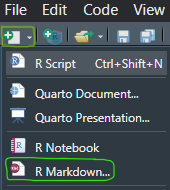
\includegraphics[width=\textwidth,height=1.45833in]{./img/rmd-click.png} \ldots{} or go to File \textgreater{} New File \textgreater{} R Markdown to create a new Rmd document.
Give it a name or keep all the defaults.
It will create a document with some demo content.
When you click the ``knit''-button below the main menu, you will need to save the file and it will create the output.
Try to play around with the text and read the demo content - it explains the basic functions!

\begin{figure}
\centering
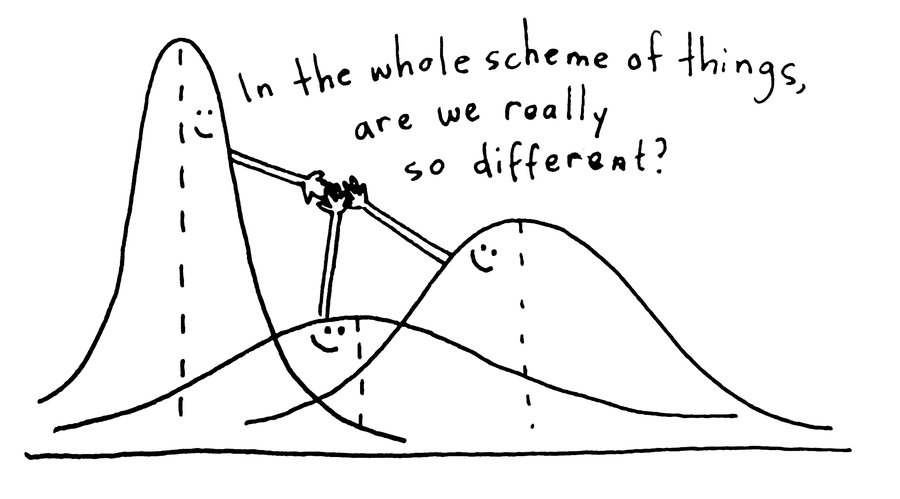
\includegraphics[width=\textwidth,height=4.47917in]{./img/sweet-anova.png}
\caption{Cute ANOVA curves}\label{id}
\end{figure}

\chapter{Creating and interpreting statistics: correlation \& regression}\label{creating-and-interpreting-statistics-correlation-regression}

\section{\texorpdfstring{Statistics Re-cap }{Statistics Re-cap }}\label{statistics-re-cap}

\begin{itemize}
\item
  What is a correlation?
\item
  What is the \emph{general linear model}, a.k.a. regression model?
\item
  What do they have in common? What makes them different?
\item
  They both give us measures of \textbf{association}
\item
  The association can be positive (the larger x, the larger y) or negative (the larger x, the smaller y)
\item
  \textbf{Correlation does not imply causation}

  \begin{itemize}
  \tightlist
  \item
    Correlation coefficient r only tells us about association, nothing about causal relation
  \item
    Regression model can check whether Y changes on the basis of X
  \end{itemize}
\end{itemize}

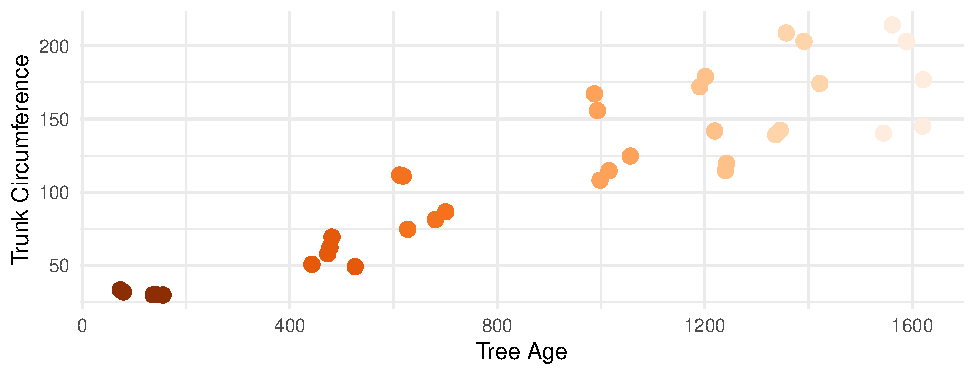
\includegraphics{_main_files/figure-latex/unnamed-chunk-73-1.pdf}

\subsection{Pre-Requisites}\label{pre-requisites-1}

\begin{itemize}
\tightlist
\item
  Load the seminar data using

  \begin{itemize}
  \tightlist
  \item
    Please make sure you are using the R dataset from the
    zip folder in ILIAS, not the original csv file we first used!
  \end{itemize}
\end{itemize}

\begin{Shaded}
\begin{Highlighting}[]
\NormalTok{seminar }\OtherTok{\textless{}{-}} \FunctionTok{readRDS}\NormalTok{(}\StringTok{"./data/seminar\_data.Rds"}\NormalTok{) }\CommentTok{\# the filepath might need adjustment for you}
\end{Highlighting}
\end{Shaded}

\begin{itemize}
\tightlist
\item
  Some of you were having trouble loading the data - please repeat the different types of data in R and the different commands used to load them! (from week 6)
\item
  \textbf{Who is having trouble opening the slides as HTML?}
\end{itemize}

\section{Correlation}\label{correlation}

\begin{itemize}
\tightlist
\item
  The pearson correlation coefficient r measures association between two numeric variables
\item
  The variables need to

  \begin{itemize}
  \tightlist
  \item
    be \emph{continuous} \& interval-scaled
  \item
    be \emph{normally distributed} \& should have \emph{no outliers}
  \item
    have a \emph{linear relationship}
  \end{itemize}
\item
  Its range is from -1 to 1

  \begin{itemize}
  \tightlist
  \item
    The closer to 0, the weaker the correlation
  \end{itemize}
\end{itemize}

\subsection{Guess the correlation!}\label{guess-the-correlation}

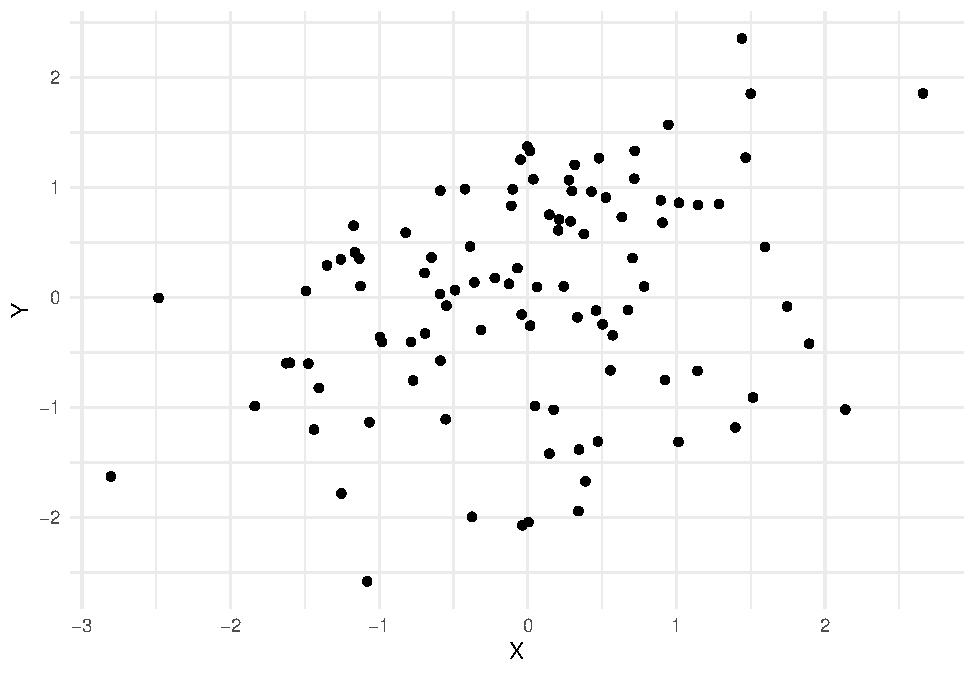
\includegraphics{_main_files/figure-latex/unnamed-chunk-75-1.pdf}

\begin{itemize}
\tightlist
\item
  r = 0.3
\end{itemize}

\section{Correlation in R}\label{correlation-in-r}

\begin{itemize}
\tightlist
\item
  Two main functions:

  \begin{itemize}
  \tightlist
  \item
    \texttt{cor()} calculates the correlation
  \item
    \texttt{cor.test()} calculates correlation and significance
  \end{itemize}
\item
  As input they both need only an x and a y variable

  \begin{itemize}
  \tightlist
  \item
    You can specify some other aspects of the calculation, such as statistical method (e.g.~``spearman'') or how to deal with missing data
  \end{itemize}
\end{itemize}

\subsection{Example}\label{example-2}

\begin{Shaded}
\begin{Highlighting}[]
\NormalTok{x }\OtherTok{\textless{}{-}} \DecValTok{1}\SpecialCharTok{:}\DecValTok{10} 
\NormalTok{y }\OtherTok{\textless{}{-}} \FunctionTok{sample}\NormalTok{(x, }\DecValTok{10}\NormalTok{)}
\FunctionTok{cor}\NormalTok{(x, y)}
\end{Highlighting}
\end{Shaded}

\begin{verbatim}
## [1] 0.1272727
\end{verbatim}

\begin{Shaded}
\begin{Highlighting}[]
\FunctionTok{cor.test}\NormalTok{(x, y)}
\end{Highlighting}
\end{Shaded}

\begin{verbatim}
## 
##  Pearson's product-moment correlation
## 
## data:  x and y
## t = 0.36293, df = 8, p-value = 0.7261
## alternative hypothesis: true correlation is not equal to 0
## 95 percent confidence interval:
##  -0.5461162  0.7007453
## sample estimates:
##       cor 
## 0.1272727
\end{verbatim}

\subsection{Handling missing data}\label{handling-missing-data}

\begin{itemize}
\item
  Many functions have an option for missing data or \texttt{NA}s

  \begin{itemize}
  \tightlist
  \item
    You can often add the argument \texttt{na.rm\ =\ TRUE} to a function for ``NA remove''
  \end{itemize}
\item
  In the \texttt{cor()} function, we define to only use complete observations
\item
\begin{Shaded}
\begin{Highlighting}[]
\NormalTok{k }\OtherTok{\textless{}{-}} \FunctionTok{c}\NormalTok{(}\DecValTok{1}\NormalTok{, }\DecValTok{2}\NormalTok{, }\DecValTok{3}\NormalTok{, }\DecValTok{4}\NormalTok{, }\DecValTok{5}\NormalTok{)}
\NormalTok{m }\OtherTok{\textless{}{-}} \FunctionTok{c}\NormalTok{(}\DecValTok{1}\NormalTok{, }\DecValTok{3}\NormalTok{, }\DecValTok{2}\NormalTok{, }\DecValTok{5}\NormalTok{, }\ConstantTok{NA}\NormalTok{) }\CommentTok{\# same length but 1 data point is missing}
\FunctionTok{cor}\NormalTok{(k, m)}
\end{Highlighting}
\end{Shaded}

\begin{verbatim}
## [1] NA
\end{verbatim}
\end{itemize}

\subsection{Handling missing data}\label{handling-missing-data-1}

\begin{itemize}
\item
  With \texttt{use\ =\ "complete.obs"} we define to only use pairs of observations that are not missing
\item
\begin{Shaded}
\begin{Highlighting}[]
\FunctionTok{cor}\NormalTok{(k, m, }\AttributeTok{use =} \StringTok{"complete.obs"}\NormalTok{)}
\end{Highlighting}
\end{Shaded}

\begin{verbatim}
## [1] 0.8315218
\end{verbatim}
\item
\begin{Shaded}
\begin{Highlighting}[]
\FunctionTok{cor}\NormalTok{(k[}\DecValTok{1}\SpecialCharTok{:}\DecValTok{4}\NormalTok{], m[}\DecValTok{1}\SpecialCharTok{:}\DecValTok{4}\NormalTok{])}
\end{Highlighting}
\end{Shaded}

\begin{verbatim}
## [1] 0.8315218
\end{verbatim}
\end{itemize}

\subsection{Exercise:}\label{exercise-8}

\subsubsection{\texorpdfstring{Is technology skill associated with seminar motivation? }{Is technology skill associated with seminar motivation?  }}\label{is-technology-skill-associated-with-seminar-motivation}

Calculate a correlation test using \texttt{cor.test()} to analyze the question.

Try to formulate an interpretation as you would report it in a thesis or paper!

\subsection{\texorpdfstring{Solution }{Solution  }}\label{solution-12}

\begin{Shaded}
\begin{Highlighting}[]
\FunctionTok{cor.test}\NormalTok{(seminar}\SpecialCharTok{$}\NormalTok{v05\_skill\_tech, seminar}\SpecialCharTok{$}\NormalTok{v10\_motivation)}
\end{Highlighting}
\end{Shaded}

\begin{verbatim}
## 
##  Pearson's product-moment correlation
## 
## data:  seminar$v05_skill_tech and seminar$v10_motivation
## t = 1.386, df = 11, p-value = 0.1932
## alternative hypothesis: true correlation is not equal to 0
## 95 percent confidence interval:
##  -0.2100186  0.7724602
## sample estimates:
##       cor 
## 0.3855856
\end{verbatim}

``With r = 0.386 there is a positive association of moderate strength between previous technological skill and motivation for the seminaR. This association is not significant (p = 0.193), likely due to the small sample size.''

\subsection{Quiz}\label{quiz}

\subsubsection{\texorpdfstring{Look at our seminar dataset by entering \texttt{str(seminar)} in the console. Which of these correlations would work?}{Look at our seminar dataset by entering str(seminar) in the console. Which of these correlations would work?}}\label{look-at-our-seminar-dataset-by-entering-strseminar-in-the-console.-which-of-these-correlations-would-work}

\begin{itemize}
\tightlist
\item
  \texttt{cor(seminar\$v02\_age,\ seminar\$v04\_bodyheight}

  \begin{itemize}
  \tightlist
  \item
    Closing bracket missing!
  \end{itemize}
\item
  \texttt{cor(seminar\$v02\_age,\ seminar\$v08\_loudness)}

  \begin{itemize}
  \tightlist
  \item
  \end{itemize}
\item
  \texttt{cor(seminar\$v08\_loudness,\ seminar\$v06\_loc)}

  \begin{itemize}
  \tightlist
  \item
  \item
    \emph{v06\_loc} has numbers, but they are recognized as characters!
  \end{itemize}
\end{itemize}

\section{Linear Regression}\label{linear-regression}

\begin{itemize}
\tightlist
\item
  Linear regression also works on numerical, normally distributed data
\item
  We assume an association, and regression can help to look for causation

  \begin{itemize}
  \tightlist
  \item
    There is one \textbf{dependent variable} y and one \textbf{independent variable} x
  \item
    In multiple linear regression, there can be several x
  \end{itemize}
\item
  Formula: \[ y = \beta_0 + \beta x + \epsilon \]
\item
  What we are essentially doing is building a model for our data and checking how well it actually fits!
\end{itemize}

\subsection{Build the model}\label{build-the-model}

\begin{itemize}
\tightlist
\item
  The R function for regression analysis is \texttt{lm()} for \emph{linear model}
\item
  It needs a ``formula'' as input - similar to the formula in the \texttt{t.test()}, we need the \textasciitilde{}

  \begin{itemize}
  \tightlist
  \item
    Read Y \textasciitilde{} X as ``Y on the basis of/ given X''
  \item
    Our dependent variable Y goes first and our independent variable(s) go after the \textasciitilde{}
  \end{itemize}
\item
  If the variables come from a data set, we need to specify data as well
\end{itemize}

\subsection{Visual Inspection}\label{visual-inspection}

\begin{Shaded}
\begin{Highlighting}[]
\FunctionTok{ggplot}\NormalTok{(Orange, }\FunctionTok{aes}\NormalTok{(}\AttributeTok{x =}\NormalTok{ age, }\AttributeTok{y =}\NormalTok{ circumference, }\AttributeTok{color =}\NormalTok{ age)) }\SpecialCharTok{+} \FunctionTok{geom\_jitter}\NormalTok{(}\AttributeTok{size =} \DecValTok{3}\NormalTok{) }\SpecialCharTok{+}
  \FunctionTok{geom\_smooth}\NormalTok{(}\AttributeTok{method =} \StringTok{"lm"}\NormalTok{, }\AttributeTok{se=}\ConstantTok{FALSE}\NormalTok{, }\AttributeTok{color=}\StringTok{"lightgray"}\NormalTok{, }
              \AttributeTok{linewidth =}\NormalTok{ .}\DecValTok{7}\NormalTok{, }\AttributeTok{formula =}\NormalTok{ y }\SpecialCharTok{\textasciitilde{}}\NormalTok{ x) }\SpecialCharTok{+} \FunctionTok{theme\_minimal}\NormalTok{() }\SpecialCharTok{+} \FunctionTok{labs}\NormalTok{(}\AttributeTok{x =} \StringTok{"Tree Age"}\NormalTok{, }\AttributeTok{y =} \StringTok{"Trunk Circumference"}\NormalTok{, }\AttributeTok{title =} \StringTok{"Do trees get thicker with age?"}\NormalTok{) }\SpecialCharTok{+} \FunctionTok{scale\_color\_distiller}\NormalTok{(}\AttributeTok{palette =} \DecValTok{7}\NormalTok{) }\SpecialCharTok{+} \FunctionTok{theme}\NormalTok{(}\AttributeTok{legend.position =} \StringTok{"none"}\NormalTok{)}
\end{Highlighting}
\end{Shaded}

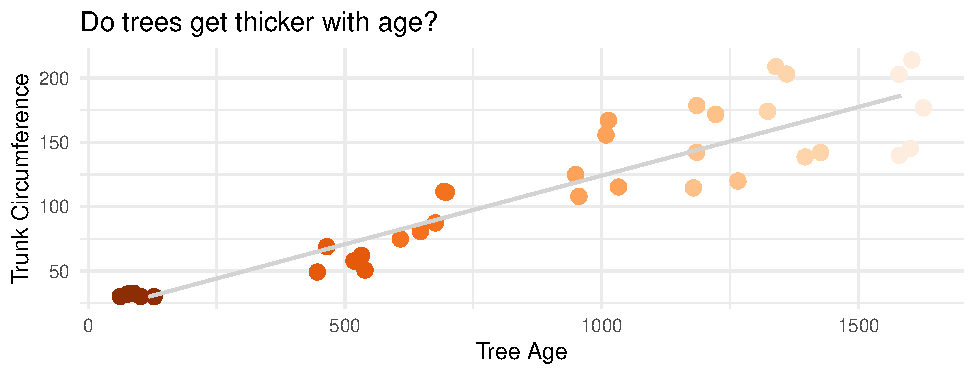
\includegraphics{_main_files/figure-latex/unnamed-chunk-81-1.pdf}

\begin{itemize}
\tightlist
\item
  What could be problematic here?

  \begin{itemize}
  \tightlist
  \item
    Heteroscedasticity
  \end{itemize}
\end{itemize}

\subsection{Build the model}\label{build-the-model-1}

\subsubsection{Do trees get thicker with age?}\label{do-trees-get-thicker-with-age}

\begin{Shaded}
\begin{Highlighting}[]
\NormalTok{Treelm }\OtherTok{\textless{}{-}} \FunctionTok{lm}\NormalTok{(}\AttributeTok{formula =}\NormalTok{ circumference }\SpecialCharTok{\textasciitilde{}}\NormalTok{ age, }\AttributeTok{data =}\NormalTok{ Orange)}
\NormalTok{Treelm}
\end{Highlighting}
\end{Shaded}

\begin{verbatim}
## 
## Call:
## lm(formula = circumference ~ age, data = Orange)
## 
## Coefficients:
## (Intercept)          age  
##     17.3997       0.1068
\end{verbatim}

\begin{itemize}
\tightlist
\item
  The lm alone gives us the mathematical formula
\item
  To look at the statistical results, we need to use another function such as \texttt{print()} or \texttt{summary()}
\end{itemize}

\subsection{Analyze the model}\label{analyze-the-model}

\begin{Shaded}
\begin{Highlighting}[]
\FunctionTok{summary}\NormalTok{(Treelm)}
\end{Highlighting}
\end{Shaded}

\begin{verbatim}
## 
## Call:
## lm(formula = circumference ~ age, data = Orange)
## 
## Residuals:
##     Min      1Q  Median      3Q     Max 
## -46.310 -14.946  -0.076  19.697  45.111 
## 
## Coefficients:
##              Estimate Std. Error t value Pr(>|t|)    
## (Intercept) 17.399650   8.622660   2.018   0.0518 .  
## age          0.106770   0.008277  12.900 1.93e-14 ***
## ---
## Signif. codes:  0 '***' 0.001 '**' 0.01 '*' 0.05 '.' 0.1 ' ' 1
## 
## Residual standard error: 23.74 on 33 degrees of freedom
## Multiple R-squared:  0.8345, Adjusted R-squared:  0.8295 
## F-statistic: 166.4 on 1 and 33 DF,  p-value: 1.931e-14
\end{verbatim}

\begin{itemize}
\tightlist
\item
  Interpretation?

  \begin{itemize}
  \tightlist
  \item
    Trees get larger circumferences the older they are, but this might be modulated by their Species, environment or other factors
  \end{itemize}
\end{itemize}

\subsection{\texorpdfstring{Exercise }{Exercise  }}\label{exercise-9}

Does the age of a person have an influence on how long they took to complete the seminar survey (session length)?

Use the \texttt{lm()} function and report the significance level of the predictor as well as the model equation.

\subsection{Solution}\label{solution-13}

\begin{Shaded}
\begin{Highlighting}[]
\NormalTok{age\_sess }\OtherTok{\textless{}{-}} \FunctionTok{lm}\NormalTok{(session\_length }\SpecialCharTok{\textasciitilde{}}\NormalTok{ v02\_age, }\AttributeTok{data =}\NormalTok{ seminar)}
\FunctionTok{summary}\NormalTok{(age\_sess)}
\end{Highlighting}
\end{Shaded}

\begin{verbatim}
## 
## Call:
## lm(formula = session_length ~ v02_age, data = seminar)
## 
## Residuals:
##     Min      1Q  Median      3Q     Max 
## -34.978  -5.605   1.209  13.395  36.141 
## 
## Coefficients:
##             Estimate Std. Error t value Pr(>|t|)  
## (Intercept)  182.706     61.517   2.970   0.0127 *
## v02_age       -4.186      2.689  -1.557   0.1478  
## ---
## Signif. codes:  0 '***' 0.001 '**' 0.01 '*' 0.05 '.' 0.1 ' ' 1
## 
## Residual standard error: 21.23 on 11 degrees of freedom
## Multiple R-squared:  0.1805, Adjusted R-squared:  0.106 
## F-statistic: 2.423 on 1 and 11 DF,  p-value: 0.1478
\end{verbatim}

\subsection{Interpretation}\label{interpretation}

``The age of a person does not significantly predict the time it took them to complete the survey (p = .148). The model equation is 182.7 -4.19X with age explaining about 18\% of the variance in session length for the survey.''

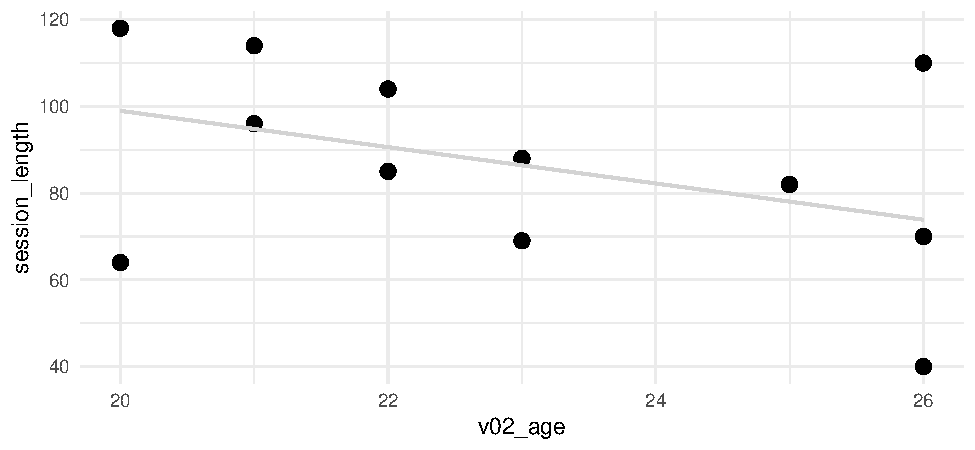
\includegraphics{_main_files/figure-latex/unnamed-chunk-85-1.pdf}

\subsection{A word to the wise}\label{a-word-to-the-wise}

\begin{itemize}
\tightlist
\item
  There is also a function called \texttt{glm()} for general linear model
\item
  In the cases I showed you, both perform the same tasks
\item
  The \texttt{glm()} can also handle other more advanced statistical analyses, including logistic regression
\item
  However, the \texttt{lm()} function will output the coefficient of determination \(R^2\)

  \begin{itemize}
  \tightlist
  \item
    It tell us the proportion of the variation in the dependent variable that is predictable from the independent variable(s)
  \item
    We \emph{could} also calculate it by hand using the \texttt{cor()} function and squaring the result
  \end{itemize}
\end{itemize}

\section{ANOVA Exercise}\label{anova-exercise}

Reminder: There are generally 3 steps to an ANOVA

\begin{Shaded}
\begin{Highlighting}[]
\NormalTok{car}\SpecialCharTok{::}\FunctionTok{leveneTest}\NormalTok{(v08\_loudness }\SpecialCharTok{\textasciitilde{}}\NormalTok{ v11\_soul, }\AttributeTok{data =}\NormalTok{ seminar) }\CommentTok{\# 1.}
\NormalTok{model }\OtherTok{\textless{}{-}} \FunctionTok{aov}\NormalTok{(v08\_loudness }\SpecialCharTok{\textasciitilde{}}\NormalTok{ v11\_soul, }\AttributeTok{data =}\NormalTok{ seminar) }\CommentTok{\# 2.}
\FunctionTok{summary}\NormalTok{(model)}
\FunctionTok{TukeyHSD}\NormalTok{(model) }\CommentTok{\# 3.}
\end{Highlighting}
\end{Shaded}

\begin{enumerate}
\def\labelenumi{\arabic{enumi}.}
\tightlist
\item
  Check assumptions with Levene Test
\item
  Build the model to perform an omnibus ANOVA
\item
  Perform post-hoc tests to check pairwise differences (usually only if the omnibus ANOVA is significant)
\end{enumerate}

\subsection{Exercise:}\label{exercise-10}

\subsubsection{\texorpdfstring{Does the preferred music volume depend on someone's soul philosophy? }{Does the preferred music volume depend on someone's soul philosophy? }}\label{does-the-preferred-music-volume-depend-on-someones-soul-philosophy}

Perform an ANOVA on our seminar data to explore the question (v08 \& v12).

Look for pairwise differences even if the overall ANOVA does not reach significance.

\subsection{\texorpdfstring{Solution }{Solution }}\label{solution-14}

\begin{Shaded}
\begin{Highlighting}[]
\NormalTok{car}\SpecialCharTok{::}\FunctionTok{leveneTest}\NormalTok{(v08\_loudness }\SpecialCharTok{\textasciitilde{}}\NormalTok{ v12\_soul\_phil, }\AttributeTok{data =}\NormalTok{ seminar)}
\end{Highlighting}
\end{Shaded}

\begin{verbatim}
## Warning in leveneTest.default(y = y, group = group, ...): group coerced to
## factor.
\end{verbatim}

\begin{verbatim}
## Levene's Test for Homogeneity of Variance (center = median)
##       Df F value Pr(>F)
## group  2  0.3112 0.7394
##       10
\end{verbatim}

\begin{Shaded}
\begin{Highlighting}[]
\NormalTok{model }\OtherTok{\textless{}{-}} \FunctionTok{aov}\NormalTok{(v08\_loudness }\SpecialCharTok{\textasciitilde{}}\NormalTok{ v12\_soul\_phil, }\AttributeTok{data =}\NormalTok{ seminar)}
\FunctionTok{summary}\NormalTok{(model)}
\end{Highlighting}
\end{Shaded}

\begin{verbatim}
##               Df Sum Sq Mean Sq F value  Pr(>F)   
## v12_soul_phil  2 1164.8   582.4   8.797 0.00625 **
## Residuals     10  662.1    66.2                   
## ---
## Signif. codes:  0 '***' 0.001 '**' 0.01 '*' 0.05 '.' 0.1 ' ' 1
\end{verbatim}

\subsection{\texorpdfstring{Solution }{Solution }}\label{solution-15}

\subsubsection{Pairwise Comparison}\label{pairwise-comparison}

\begin{Shaded}
\begin{Highlighting}[]
\FunctionTok{TukeyHSD}\NormalTok{(model)}
\end{Highlighting}
\end{Shaded}

\begin{verbatim}
##   Tukey multiple comparisons of means
##     95% family-wise confidence level
## 
## Fit: aov(formula = v08_loudness ~ v12_soul_phil, data = seminar)
## 
## $v12_soul_phil
##                      diff        lwr       upr     p adj
## dunno-dualism    9.714286  -5.678116 25.106687 0.2419042
## monism-dualism -13.666667 -31.879202  4.545868 0.1490289
## monism-dunno   -23.380952 -38.773354 -7.988551 0.0049965
\end{verbatim}

\subsection{\texorpdfstring{If there is still time: }{If there is still time: }}\label{if-there-is-still-time}

Choose and create an appropriate visualization for this data!

\subsection{\texorpdfstring{Data Viz }{Data Viz }}\label{data-viz}

\begin{Shaded}
\begin{Highlighting}[]
\FunctionTok{ggplot}\NormalTok{(seminar, }\FunctionTok{aes}\NormalTok{(}\AttributeTok{x =}\NormalTok{ v12\_soul\_phil, }\AttributeTok{y =}\NormalTok{ v08\_loudness, }
                    \AttributeTok{color =}\NormalTok{ v12\_soul\_phil, }\AttributeTok{fill =}\NormalTok{ v12\_soul\_phil)) }\SpecialCharTok{+}
  \FunctionTok{geom\_boxplot}\NormalTok{(}\AttributeTok{alpha =}\NormalTok{ .}\DecValTok{7}\NormalTok{) }\SpecialCharTok{+} \FunctionTok{theme\_minimal}\NormalTok{() }\SpecialCharTok{+} \FunctionTok{theme}\NormalTok{(}\AttributeTok{legend.position =} \StringTok{"none"}\NormalTok{) }\SpecialCharTok{+}
  \FunctionTok{labs}\NormalTok{(}\AttributeTok{x =} \StringTok{"Soul Philosophy"}\NormalTok{, }\AttributeTok{y =} \StringTok{"Preferred Volume (arbitrary units)"}\NormalTok{) }\SpecialCharTok{+}
  \FunctionTok{scale\_color\_brewer}\NormalTok{(}\AttributeTok{palette =} \DecValTok{4}\NormalTok{) }\SpecialCharTok{+} \FunctionTok{scale\_fill\_brewer}\NormalTok{(}\AttributeTok{palette =} \DecValTok{4}\NormalTok{)}
\end{Highlighting}
\end{Shaded}

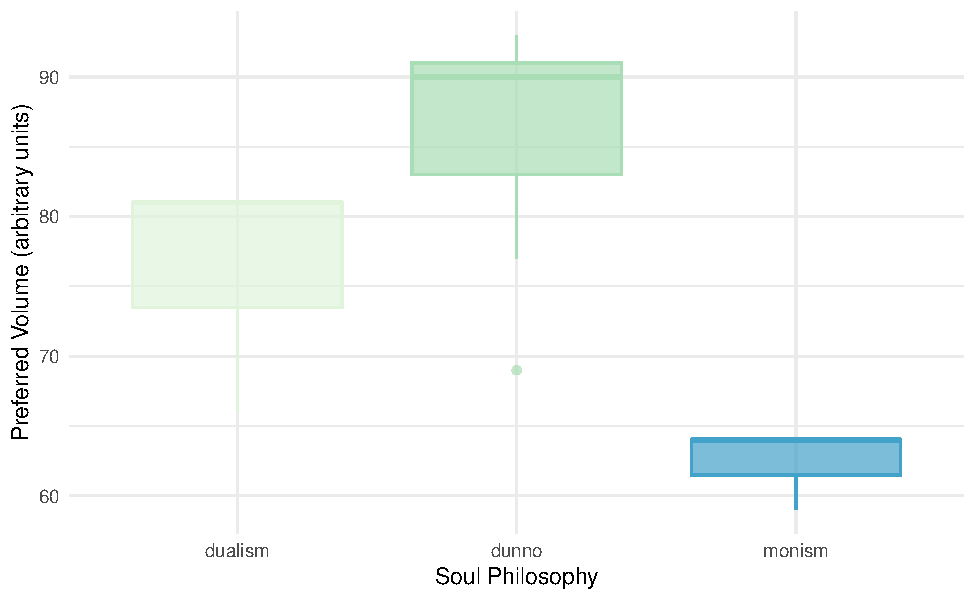
\includegraphics{_main_files/figure-latex/unnamed-chunk-89-1.pdf}

\section{Wrap-Up \& Further Resources}\label{wrap-up-further-resources-7}

Correlation coefficient \emph{r} can be determined using \texttt{cor(x,y)}

\(R^2\) is the coefficient of determination in a linear model (calculate by hand or in the model formula)

The linear model function \texttt{lm()} is used to build models for linear regression

Problems such as overfitting or heteroscedasticity reduce the interpretability of the model results

\href{https://www.guessthecorrelation.com/}{Guess the Correlation}

\href{https://statisticsbyjim.com/basics/correlation-coefficient-formula/}{Explanation: Correlation}

\href{https://www.datacamp.com/tutorial/linear-regression-R}{Linear Regression in R}

\href{https://www.codecademy.com/learn/learn-linear-regression-in-r/modules/linear-regression-in-r/cheatsheet/}{lm() cheatsheet}

\begin{Shaded}
\begin{Highlighting}[]
\FunctionTok{ggplot}\NormalTok{(Orange, }\FunctionTok{aes}\NormalTok{(}\AttributeTok{x =}\NormalTok{ age, }\AttributeTok{y =}\NormalTok{ circumference, }\AttributeTok{color =}\NormalTok{ Tree)) }\SpecialCharTok{+}
  \FunctionTok{geom\_point}\NormalTok{(}\AttributeTok{size =} \DecValTok{3}\NormalTok{) }\SpecialCharTok{+} \FunctionTok{labs}\NormalTok{(}\AttributeTok{x =} \StringTok{"Tree Age"}\NormalTok{, }\AttributeTok{y =} \StringTok{"Trunk Circumference"}\NormalTok{) }\SpecialCharTok{+}
  \FunctionTok{geom\_line}\NormalTok{(}\FunctionTok{aes}\NormalTok{(}\AttributeTok{color =}\NormalTok{ Tree)) }\SpecialCharTok{+} \FunctionTok{theme\_minimal}\NormalTok{() }\SpecialCharTok{+} \FunctionTok{theme}\NormalTok{(}\AttributeTok{legend.position =} \StringTok{"none"}\NormalTok{)}
\end{Highlighting}
\end{Shaded}

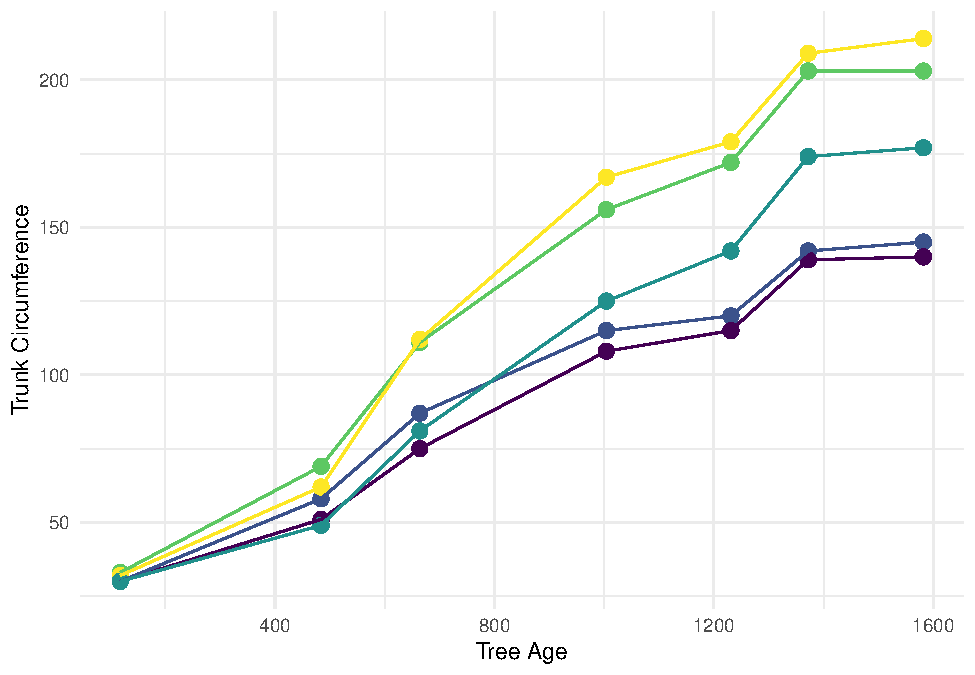
\includegraphics{_main_files/figure-latex/unnamed-chunk-90-1.pdf}

\chapter{Intro to R Markdown}\label{intro-to-r-markdown}

\begin{figure}
\centering

\includegraphics{./img/rmd.png}
\caption{R Markdown Logo}
\end{figure}

\section{Creating whole documents in R}\label{creating-whole-documents-in-r}

\begin{itemize}
\tightlist
\item
  Creating visualizations and statistics in R is great, but we need to able to show and report our work.
\item
  Results can be copied and plots can be exported, but they can also be embedded directly into a document in R
\item
  R Markdown is a text engine based on \(\LaTeX\) that allows you to create documents, presentations, reports\ldots{}
\end{itemize}

\begin{figure}
\centering
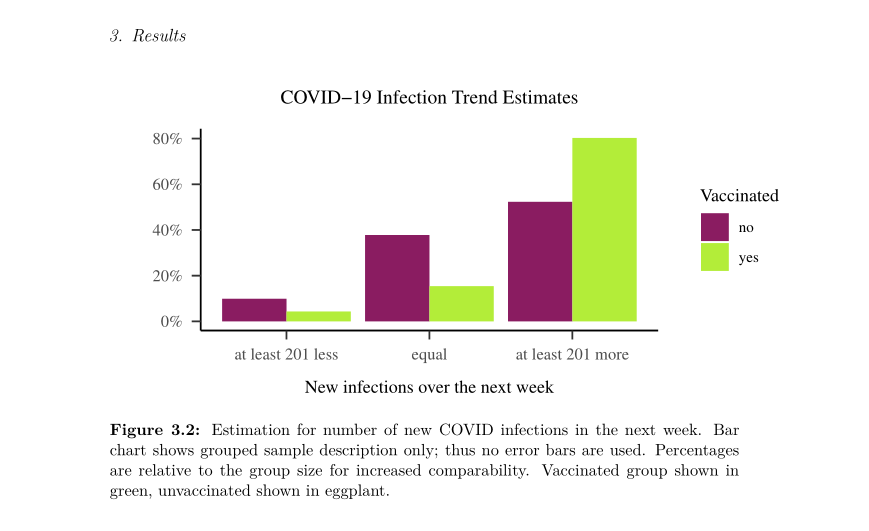
\includegraphics[width=\textwidth,height=2.60417in]{./img/MArmdex.png}
\caption{MA thesis Example}
\end{figure}

\subsection{Example}\label{example-3}

\begin{itemize}
\tightlist
\item
  You've hopefully all tried out creating your own R Markdown document as homework
\item
  We'll all create a new RMarkdown document now and augment that as we go on with this class!
\item
  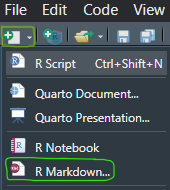
\includegraphics[width=\textwidth,height=1.45833in]{./img/rmd-click.png} \ldots{} or go to File \textgreater{} New File \textgreater{} R Markdown to create a new markdown document
\item
  \textbf{Let's try that out!}
\end{itemize}

\section{Document Basics}\label{document-basics}

\begin{itemize}
\tightlist
\item
  RMarkdown has some basics that need to be learned
\item
  It also has many features and powerful tools for layout and styling
\item
  By default, RMarkdown can create html documents - if you want a pdf, you need a special package to render \(\LaTeX\), I recommend \texttt{tinytex}

  \begin{itemize}
  \tightlist
  \item
    \texttt{install.packages("tinytex")}
  \item
    \texttt{tinytex::install\_tinytex()}
  \end{itemize}
\end{itemize}

\subsection{\texorpdfstring{YAML header (\emph{Yet Another Markdown Language})}{YAML header (Yet Another Markdown Language)}}\label{yaml-header-yet-another-markdown-language}

\begin{itemize}
\item
  This defines the output format of our document, e.g.~\texttt{html\_document}
\item
  We can set our title, subtitle, author, date\ldots{}
\item
  We can define further characteristics, e.g.~\texttt{toc} (table of content) or \texttt{self-contained} (this should be set to true, otherwise R will not copy images etc. and the document will not work properly on other devices)
\item
  The YAML header needs to be indented in a certain way, otheriwse the commands are not recognized!
\item
  In the YAML header, \texttt{true} and \texttt{false} are not capitalized, unlike in the rest of R!
\end{itemize}

\subsection{Markdown Basics}\label{markdown-basics}

Text formatting generally works with characters in the text:

\begin{itemize}
\tightlist
\item
  \emph{italics} with \_italics\_
\item
  \textbf{bold} with **bold**
\item
  \textbf{\emph{bold and cursive}} with **\_bold and cursive\_**
\item
  Unordered lists are created with -
\item
  Ordered lists with 1., 2. \ldots{}
\end{itemize}

\section{\#\# Heading Basics}\label{heading-basics}

\subsection{\#\#\# Sub Header 3. level}\label{sub-header-3.-level}

\subsubsection{\#\#\#\# 4th level}\label{th-level}

\paragraph{\#\#\#\#\# 5th level}\label{th-level-1}

\subparagraph{\#\#\#\#\#\# 6th level}\label{th-level-2}

Thats's it.

Realistically, we \emph{may} want to go down to the 4th level heading, but usually no further.

\section{Special Features}\label{special-features}

\begin{itemize}
\tightlist
\item
  Print mathematical equations
\item
  Show code and its output
\item
  Easily use automatic formatting
\item
  Profit from existing templates
\item
  General rule of thumb: Rmd documents are rendered depending on their output format

  \begin{itemize}
  \tightlist
  \item
    If you plan on creating an html, you can use plain html to make adjustments and use special features.
  \item
    If you create a pdf, they will most likely not work and you should use \(\LaTeX\) notation.
  \end{itemize}
\end{itemize}

\subsection{\texorpdfstring{\(\LaTeX\)}{\textbackslash LaTeX}}\label{latex}

Especially useful for writing equations:

\begin{itemize}
\tightlist
\item
  \$ \textbackslash{} alpha \$ \(\rightarrow\) \(\alpha\)
\item
  \$ \textbackslash{} beta \$ \(\rightarrow\) \(\beta\)
\item
  \$ R\^{}2 \$ \(\rightarrow\) \(R^2\)
\item
  and, by the way, \$ \textbackslash{} rightarrow \$ becomes \(\rightarrow\)
\item
  and \$ \textbackslash{} LaTeX \$ becomes \(\LaTeX\)
\item
  \textbackslash{} newline creates a new line and \textbackslash{} newpage creates a new page
\end{itemize}

\subsection{HTML}\label{html}

Remember these tags should only be used when creating a html document!

\begin{itemize}
\tightlist
\item
  \textless{} br \textgreater{} creates a new line (stands for ``line break'')
\item
  \textless span style=``color: purple;''\textgreater{} This text will appear purple. \textless/span\textgreater{}

  \begin{itemize}
  \tightlist
  \item
    { This text will appear purple. }
  \end{itemize}
\item
  Simple tables can be created with html notation in most documents

  \begin{itemize}
  \tightlist
  \item
    Header 1 \textbar{} Header 2
  \item
    \emph{then a row of - - - \textbar{} - - - to represent the lines}
  \item
    And the content separated \textbar{} into as many columns as defined
  \end{itemize}
\end{itemize}

\subsection{Table Example}\label{table-example}

Header 1 \textbar{} Header 2
-----\textbar-----
Great content \textbar{} Fantastic content

Becomes:

\begin{longtable}[]{@{}ll@{}}
\toprule\noalign{}
Header 1 & Header 2 \\
\midrule\noalign{}
\endhead
\bottomrule\noalign{}
\endlastfoot
Great content & Fantastic content \\
\end{longtable}

\section{Including R}\label{including-r}

\begin{itemize}
\tightlist
\item
  Including R code can be achieved by either inserting so-called code chunks or using inline code
\item
  Code chunks are useful if several lines of code need to be evaluated and/ or shown

  \begin{itemize}
  \tightlist
  \item
    There are many options for code chunks
  \end{itemize}
\item
  Inline code is useful if single outputs are to be shown

  \begin{itemize}
  \tightlist
  \item
    E.g. with functions you already know such as \texttt{apa\_print()}
  \end{itemize}
\end{itemize}

\subsection{Code Chunks}\label{code-chunks}

\begin{itemize}
\item
  Code chunks are inserted via the menu Code \textgreater{} Insert Chunk and should look like this:
\item
  ```\{r\}
  \# \emph{code goes here}
  ```
\item
\begin{Shaded}
\begin{Highlighting}[]
\CommentTok{\# code goes here}
\end{Highlighting}
\end{Shaded}
\item
  Or you can use the keyboard shortcut ctrl + alt + i / command + option + i
\end{itemize}

\subsection{Chunk Options}\label{chunk-options}

\begin{itemize}
\item
  Inside the curly brackets, you can specify many different options, for example:

  \begin{itemize}
  \tightlist
  \item
    \texttt{fig.height\ =\ 3} will output a plot to a certain height (3 inches)
  \item
    \texttt{echo\ =\ F} will show code output, but not the code
  \item
    \texttt{eval\ =\ F} will show the code, but not its' output\ldots{}
  \end{itemize}
\item
  eval = F:

\begin{Shaded}
\begin{Highlighting}[]
\FunctionTok{head}\NormalTok{(iris, }\DecValTok{1}\NormalTok{) }
\end{Highlighting}
\end{Shaded}
\item
  echo = F:

\begin{verbatim}
##   Sepal.Length Sepal.Width Petal.Length Petal.Width Species
## 1          5.1         3.5          1.4         0.2  setosa
\end{verbatim}
\end{itemize}

\subsection{Chunk Options:}\label{chunk-options-1}

\subsubsection{\texorpdfstring{\texttt{error\ =\ TRUE}}{error = TRUE}}\label{error-true}

\begin{itemize}
\tightlist
\item
  This option allows us to include erroneous code in our script
\item
  It will output the error message just like you would see in your R Studio console
\item
  By default, \texttt{error\ =\ FALSE} which means that your script cannot be rendered with errors in code chunks
\end{itemize}

\begin{Shaded}
\begin{Highlighting}[]
\FunctionTok{mean}\NormalTok{(y)}
\end{Highlighting}
\end{Shaded}

\begin{verbatim}
## [1] 5.5
\end{verbatim}

\section{Wrap-Up \& Further Resources}\label{wrap-up-further-resources-8}

RMarkdown allows you to create professional documents

You can use it like other text-generating programs (e.g.~MS Word)

Embed plots, code and statistical results directly in your document

Show equations and use other special features

\href{https://www.youtube.com/watch?v=asHhuHRxhvo&ab_channel=EquitableEquations/}{YouTube: What is R Markdown?}

\href{https://wch.github.io/latexsheet/}{LaTeX Cheatsheet}

\href{https://web.stanford.edu/group/csp/cs21/htmlcheatsheet.pdf}{HTML Cheatsheet}

\href{https://bookdown.org/yihui/rmarkdown-cookbook/}{RMarkdown Cookbook}

\href{https://yihui.org/knitr/options/}{RMarkdown Chunk Options}

\href{https://www.youtube.com/watch?v=01KifhHDkFk&ab_channel=EquitableEquations}{YouTube: Presentations with Quarto}

\begin{figure}
\centering

\includegraphics[width=\textwidth,height=5.72917in]{img/shakespeare.jpg}
\caption{Shakespeare writing RMarkdown}
\end{figure}

\chapter{Taking full Advantage of R and R Markdown}\label{taking-full-advantage-of-r-and-r-markdown}

\begin{figure}
\centering

\includegraphics{./img/papaja.png}
\caption{Happy Papaya Logo}
\end{figure}

\section{Quiz - Rmd specific}\label{quiz---rmd-specific}

\begin{enumerate}
\def\labelenumi{\arabic{enumi}.}
\tightlist
\item
  What do I need to do to make my text \textbf{\emph{look like this}}?

  \begin{itemize}
  \tightlist
  \item
    **\_look like this\_**
  \end{itemize}
\item
  I want to add a subtitle to my document, where might I do that?

  \begin{itemize}
  \tightlist
  \item
    Add `subtitle: ``A great subtitle''\,' to the \textbf{YAML header}
  \end{itemize}
\item
  How do I generate a section header in my document?

  \begin{itemize}
  \tightlist
  \item
    With the pound sign \# Header
  \end{itemize}
\item
  Oh no, my header isn't showing up right! What could have happened?

  \begin{itemize}
  \tightlist
  \item
    There needs to be a space between the \# and the header
  \end{itemize}
\end{enumerate}

\subsection{Quiz - general R}\label{quiz---general-r}

\begin{enumerate}
\def\labelenumi{\arabic{enumi}.}
\item
  What package contains the functions \texttt{select,\ filter\ \&\ mutate}?

  \begin{itemize}
  \tightlist
  \item
    \texttt{dplyr} (or \texttt{tidyverse})
  \end{itemize}
\item
  Assume I have created some R project and I read a file with the following command - what does this tell you about the folder on my computer?

\begin{Shaded}
\begin{Highlighting}[]
\NormalTok{greatdata }\OtherTok{\textless{}{-}}\NormalTok{ readr}\SpecialCharTok{::}\FunctionTok{read\_csv}\NormalTok{(}\AttributeTok{file =} \StringTok{"./data/somefile.CSV"}\NormalTok{)}
\end{Highlighting}
\end{Shaded}

  \begin{itemize}
  \tightlist
  \item
    The folder containing the R project contains a subfolder called ``data'' and in there is a CSV file called ``somefile.csv''.
  \end{itemize}
\end{enumerate}

\subsection{Quiz - general R}\label{quiz---general-r-1}

\begin{enumerate}
\def\labelenumi{\arabic{enumi}.}
\setcounter{enumi}{2}
\tightlist
\item
  I want to load a csv file into R with \texttt{readRDS()}. Why isn't it working?

  \begin{itemize}
  \tightlist
  \item
    The read commands are specific to the file format. readRDS() is for R files, read.csv() or readr::read\_csv() are needed for csv files
  \end{itemize}
\item
  What do you know when you look at the command \texttt{bigfive\$extraversion}?

  \begin{itemize}
  \tightlist
  \item
    There is a data set called \texttt{bigfive} and we're accessing a variable called \texttt{extraversion}
  \end{itemize}
\end{enumerate}

\subsection{Quiz - general R}\label{quiz---general-r-2}

\begin{enumerate}
\def\labelenumi{\arabic{enumi}.}
\setcounter{enumi}{4}
\item
  What keywords for loops and conditionals do you remember?

  \begin{itemize}
  \tightlist
  \item
    \emph{for, while, if, else, ifelse}\ldots{}
  \end{itemize}
\item
  I want to calculate a t-test on soul-belief (yes or no) and age in our seminar data. Why won't this command work?

\begin{Shaded}
\begin{Highlighting}[]
\FunctionTok{t.test}\NormalTok{(v02\_age, soul\_dummy, }\AttributeTok{data =}\NormalTok{ seminar)}
\end{Highlighting}
\end{Shaded}

  \begin{itemize}
  \tightlist
  \item
    When we have a grouping variable like soul\_dummy, we need to use formula notation: \texttt{v02\_age\ \textasciitilde{}\ soul\_dummy}
  \end{itemize}
\end{enumerate}

\section{Back to Rmd: Last session}\label{back-to-rmd-last-session}

\begin{itemize}
\tightlist
\item
  First off: the option of formatting the table of contents to float in html is \textbf{toc\_float: true}
\item
  Create Rmd: 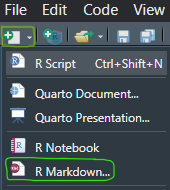
\includegraphics[width=\textwidth,height=1.04167in]{./img/rmd-click.png} or File \textgreater{} New File \textgreater{} R Markdown
\item
  \textbf{YAML header} defines format of the document as well as key info such as title, date, etc.
\item
  Text formatting:

  \begin{itemize}
  \tightlist
  \item
    \emph{italics} with \_italics\_
  \item
    \textbf{bold} with **bold**
  \item
    Unordered lists are created with -
  \item
    Ordered lists with 1., 2. \ldots{}
  \end{itemize}
\end{itemize}

\subsection{Last session}\label{last-session}

\begin{itemize}
\tightlist
\item
  Code chunks are inserted via the menu Code \textgreater{} Insert Chunk and should look like this:
\item
  ```\{r\}
  \# \emph{code goes here}
  ```

  \begin{itemize}
  \tightlist
  \item
    keyboard shortcut ctrl + alt + i / command + option + i
  \item
    Chunk options can specify how to treat code, e.g.~\texttt{echo\ =\ FALSE} only shows output but does not ``echo'' the actual code
  \end{itemize}
\item
  Indentation and spacing is very important! In the text, it is better to add more. In the YAML header, it may not be recognized properly with improper spacing
\end{itemize}

\subsection{Including Links \& Images}\label{including-links-images}

\begin{itemize}
\item
  An image to R Markdown is essentially a \textbf{link to an image file on your computer}

  \begin{itemize}
  \tightlist
  \item
    That's why they share similar notation
  \end{itemize}
\item
  \begin{longtable}[]{@{}l@{}}
  \toprule\noalign{}
  Web Link:** \\
  \midrule\noalign{}
  \endhead
  \bottomrule\noalign{}
  \endlastfoot
  ``\href{www.google.com}{Google Link}'' \\
  \end{longtable}

  \begin{itemize}
  \tightlist
  \item
    Becomes: \href{https://www.google.com/}{Google Link} (clickable Link)
  \end{itemize}
\item
  \textbf{Image:}

  \begin{itemize}
  \tightlist
  \item
    ``\includegraphics{C:/path/to/your/image.png}''
  \item
    Different file formats, such as JPG, PNG, SVG or GIF
  \end{itemize}
\item
  When including an image, make sure you are using the right file path, image name \& file extension! So that\ldots{}
\item
  ``
\includegraphics{"./img/rmd.png"}''
\item
  \ldots becomes\ldots{}
\item
  \begin{figure}
  \centering
  
\includegraphics{./img/rmd.png}
  \caption{RMarkdown Logo}
  \end{figure}
\end{itemize}

\subsection{Inline Code}\label{inline-code}

\begin{itemize}
\tightlist
\item
  To simply include variables or values in text, we can use inline code `\emph{r code} `
\item
  Simply type one back tick ` and r - the program will auto complete the command
\item
  Examples:

  \begin{itemize}
  \tightlist
  \item
    The average sepal length of iris flowers is
    `\emph{r mean(iris\$Sepal.Length)}` \(\rightarrow\) 5.843
  \end{itemize}
\end{itemize}

\section{Taking full advantage of R}\label{taking-full-advantage-of-r}

\begin{enumerate}
\def\labelenumi{\arabic{enumi}.}
\tightlist
\item
  Conduct Analysis, e.g.~an ANOVA
\item
  Write about your analysis \& report results (with proper statistics)
\item
  Choose and create an appropriate visualization, e.g.~a boxplot
\end{enumerate}

\subsection{Walkthrough}\label{walkthrough}

We will use the package \texttt{palmerpenguins} (\texttt{install.packages("palmerpenguins")}) and see whether penguins from different islands have different body mass.

\begin{Shaded}
\begin{Highlighting}[]
\FunctionTok{library}\NormalTok{(palmerpenguins)}

\CommentTok{\# Test assumption of homoscedasticity}
\NormalTok{car}\SpecialCharTok{::}\FunctionTok{leveneTest}\NormalTok{(}\FunctionTok{aov}\NormalTok{(bill\_length\_mm }\SpecialCharTok{\textasciitilde{}}\NormalTok{ species, }\AttributeTok{data =}\NormalTok{ penguins)) }\CommentTok{\# yay}
\end{Highlighting}
\end{Shaded}

\begin{verbatim}
## Levene's Test for Homogeneity of Variance (center = median)
##        Df F value Pr(>F)
## group   2  2.2425 0.1078
##       339
\end{verbatim}

\begin{Shaded}
\begin{Highlighting}[]
\CommentTok{\# Run \& save ANOVA}
\NormalTok{penguinmodel }\OtherTok{\textless{}{-}} \FunctionTok{aov}\NormalTok{(bill\_length\_mm }\SpecialCharTok{\textasciitilde{}}\NormalTok{ species, }\AttributeTok{data =}\NormalTok{ penguins)}
\end{Highlighting}
\end{Shaded}

\subsection{Walkthrough}\label{walkthrough-1}

\begin{Shaded}
\begin{Highlighting}[]
\CommentTok{\# Run \& save post{-}hoc Tests}
\FunctionTok{TukeyHSD}\NormalTok{(penguinmodel)}
\end{Highlighting}
\end{Shaded}

\begin{verbatim}
##   Tukey multiple comparisons of means
##     95% family-wise confidence level
## 
## Fit: aov(formula = bill_length_mm ~ species, data = penguins)
## 
## $species
##                       diff       lwr        upr     p adj
## Chinstrap-Adelie 10.042433  9.024859 11.0600064 0.0000000
## Gentoo-Adelie     8.713487  7.867194  9.5597807 0.0000000
## Gentoo-Chinstrap -1.328945 -2.381868 -0.2760231 0.0088993
\end{verbatim}

\begin{itemize}
\item
  For anova, we want to report the full statistics, a.k.a ``full\_result'' from \texttt{papaja::apa\_print()}
\item
\begin{Shaded}
\begin{Highlighting}[]
\FunctionTok{library}\NormalTok{(papaja)}
\NormalTok{apa\_result }\OtherTok{\textless{}{-}} \FunctionTok{apa\_print}\NormalTok{(penguinmodel)}\SpecialCharTok{$}\NormalTok{full\_result}
\end{Highlighting}
\end{Shaded}
\end{itemize}

\subsection{Walkthrough}\label{walkthrough-2}

Create a boxplot and add results right in the caption!

\begin{Shaded}
\begin{Highlighting}[]
\FunctionTok{library}\NormalTok{(ggplot2)}
\FunctionTok{ggplot}\NormalTok{(penguins, }\FunctionTok{aes}\NormalTok{(}\AttributeTok{x=}\NormalTok{species, }\AttributeTok{y=}\NormalTok{bill\_length\_mm, }\AttributeTok{color=}\NormalTok{species, }\AttributeTok{fill=}\NormalTok{species), }\AttributeTok{na.rm=}\NormalTok{T) }\SpecialCharTok{+}
  \FunctionTok{geom\_boxplot}\NormalTok{(}\AttributeTok{alpha =}\NormalTok{ .}\DecValTok{7}\NormalTok{) }\SpecialCharTok{+} \FunctionTok{theme\_apa}\NormalTok{() }\SpecialCharTok{+} \FunctionTok{theme}\NormalTok{(}\AttributeTok{legend.position =} \StringTok{"none"}\NormalTok{) }\SpecialCharTok{+}
  \FunctionTok{labs}\NormalTok{(}\AttributeTok{x =} \StringTok{"Penguin Species"}\NormalTok{, }\AttributeTok{y =} \StringTok{"Bill Length (mm)"}\NormalTok{, }
       \AttributeTok{caption =}\NormalTok{ latex2exp}\SpecialCharTok{::}\FunctionTok{TeX}\NormalTok{(}\FunctionTok{unlist}\NormalTok{(apa\_result))) }\SpecialCharTok{+}
  \FunctionTok{scale\_color\_brewer}\NormalTok{(}\AttributeTok{palette =} \DecValTok{5}\NormalTok{) }\SpecialCharTok{+}
  \FunctionTok{scale\_fill\_brewer}\NormalTok{(}\AttributeTok{palette =} \DecValTok{5}\NormalTok{)}
\end{Highlighting}
\end{Shaded}

\includegraphics{_main_files/figure-latex/unnamed-chunk-104-1.pdf}

\subsection{Walkthrough}\label{walkthrough-3}

\begin{itemize}
\tightlist
\item
  Note that it is a little complex to include the result right in the caption

  \begin{itemize}
  \tightlist
  \item
    ggplot2 cannot handle \(\LaTeX\) notation so we need to use package latex2exp
  \item
    the TeX function from that package cannot handle the list-output from apa\_print()\$full\_result so we need to ``unlist'' that
  \end{itemize}
\item
  Using RMarkdown, it is much easier to include the statistic right in the text with inline code:

  \begin{itemize}
  \tightlist
  \item
    `\emph{r apa\_print(penguinmodel)\$full\_result}`
  \item
    \(\rightarrow\) { \(F(2, 339) = 410.60\), \(p < .001\), \(\hat{\eta}^2_G = .708\), 90\% CI \([.669, .740]\) }
  \end{itemize}
\end{itemize}

\section{Exercise}\label{exercise-11}

Create an R Markdown Document that includes the same type of analyses of variance with all steps that we have conducted before.
Please use the \texttt{penguins} dataset from the \texttt{palmerpenguins} package and take ``species'' as the independet variable and ``flipper\_length\_mm'' as the dependent variable.

\subsection{Exercise}\label{exercise-12}

\subsubsection{Code Solution}\label{code-solution}

\begin{Shaded}
\begin{Highlighting}[]
\FunctionTok{leveneTest}\NormalTok{(}\FunctionTok{aov}\NormalTok{(flipper\_length\_mm }\SpecialCharTok{\textasciitilde{}}\NormalTok{ species, }\AttributeTok{data =}\NormalTok{ penguins))}
\NormalTok{penguinmodel2 }\OtherTok{\textless{}{-}} \FunctionTok{aov}\NormalTok{(bill\_length\_mm }\SpecialCharTok{\textasciitilde{}}\NormalTok{ species, }\AttributeTok{data =}\NormalTok{ penguins)}
\NormalTok{posthoc }\OtherTok{\textless{}{-}} \FunctionTok{TukeyHSD}\NormalTok{(penguinmodel2)}
\NormalTok{apa\_result }\OtherTok{\textless{}{-}} \FunctionTok{apa\_print}\NormalTok{(penguinmodel2)}\SpecialCharTok{$}\NormalTok{full\_result}

\FunctionTok{ggplot}\NormalTok{(penguins) }\SpecialCharTok{+}
  \FunctionTok{geom\_boxplot}\NormalTok{(}\FunctionTok{aes}\NormalTok{(}\AttributeTok{x =}\NormalTok{ species, }\AttributeTok{y =}\NormalTok{ flipper\_length\_mm, }\AttributeTok{color =}\NormalTok{ species, }\AttributeTok{fill =}\NormalTok{ species), }
               \AttributeTok{alpha =}\NormalTok{ .}\DecValTok{7}\NormalTok{, }\AttributeTok{na.rm =} \ConstantTok{TRUE}\NormalTok{) }\SpecialCharTok{+}
  \FunctionTok{theme\_apa}\NormalTok{() }\SpecialCharTok{+} 
  \FunctionTok{theme}\NormalTok{(}\AttributeTok{legend.position =} \StringTok{"none"}\NormalTok{) }\SpecialCharTok{+}
  \FunctionTok{labs}\NormalTok{(}\AttributeTok{x =} \StringTok{"Penguin Species"}\NormalTok{, }\AttributeTok{y =} \StringTok{"Flipper Length (mm)"}\NormalTok{) }\SpecialCharTok{+}
  \FunctionTok{scale\_color\_brewer}\NormalTok{(}\AttributeTok{palette =} \DecValTok{5}\NormalTok{) }\SpecialCharTok{+}
  \FunctionTok{scale\_fill\_brewer}\NormalTok{(}\AttributeTok{palette =} \DecValTok{5}\NormalTok{)}
\end{Highlighting}
\end{Shaded}

\section{Wrap-Up \& Further Resources}\label{wrap-up-further-resources-9}

Wrap-Up

Rmd offers many options for customization

Analyses can be conducted and reported in the same document

We can profit from many automatizations, e.g.~chapter numbering

Single values/ results can be reported with inline code

Further Resources

\href{https://www.markdownguide.org/basic-syntax/}{MarkdownGuide}

\href{https://www.markdownguide.org/cheat-sheet/}{Another Markdown Cheatsheet}

\href{https://statisticsglobe.com/ggsignif-package-r}{ggsignif package example}

\href{https://bookdown.org/yihui/rmarkdown-cookbook/bibliography.html}{Bibliography and Citation}

\begin{figure}
\centering
\includegraphics[width=\textwidth,height=4.6875in]{./img/palmer_penguins.png}
\caption{Palmer Penguins}\label{id}
\end{figure}

\chapter{Wrap Up}\label{wrap-up}

\section{Discussion of Self-Study Materials}\label{discussion-of-self-study-materials}

\begin{itemize}
\tightlist
\item
  Solutions to the quiz will be uploaded on ILIAS
\item
  Specific questions, Fibonacci task, the template HTML and any additional questions
\end{itemize}

\begin{figure}
\centering
\includegraphics[width=\textwidth,height=3.125in]{./img/fibonacci.jpg}
\caption{Fibonacci Spiral}
\end{figure}

\subsection{Fibonacci Task}\label{fibonacci-task}

\begin{itemize}
\tightlist
\item
  Thanks to whoever the rest of you copied! ;)
\item
  Most of you used \texttt{numeric(15)} to create a variable with 15 zeros

  \begin{itemize}
  \tightlist
  \item
    This is fair enough, but can lead to errors: If it contains numbers already, it is harder to detect calculation mistakes (0 is often a valid possibility)
  \item
    Better to use NAs to create a placeholder variable: \texttt{rep(NA,\ X)}
  \item
  \end{itemize}

\begin{Shaded}
\begin{Highlighting}[]
\FunctionTok{rep}\NormalTok{(}\ConstantTok{NA}\NormalTok{, }\DecValTok{15}\NormalTok{)}
\end{Highlighting}
\end{Shaded}

\begin{verbatim}
##  [1] NA NA NA NA NA NA NA NA NA NA NA NA NA NA NA
\end{verbatim}
\end{itemize}

\subsection{Fibonacci Task}\label{fibonacci-task-1}

\begin{Shaded}
\begin{Highlighting}[]
\NormalTok{n }\OtherTok{\textless{}{-}} \DecValTok{15}

\NormalTok{fibonacci }\OtherTok{\textless{}{-}} \FunctionTok{c}\NormalTok{(}\DecValTok{1}\NormalTok{, }\DecValTok{1}\NormalTok{, }\FunctionTok{rep}\NormalTok{(}\ConstantTok{NA}\NormalTok{, n}\DecValTok{{-}2}\NormalTok{))}

\ControlFlowTok{for}\NormalTok{(i }\ControlFlowTok{in} \DecValTok{3}\SpecialCharTok{:}\NormalTok{n)\{}
\NormalTok{  fibonacci[i] }\OtherTok{\textless{}{-}}\NormalTok{ fibonacci[i}\DecValTok{{-}1}\NormalTok{] }\SpecialCharTok{+}\NormalTok{ fibonacci[i}\DecValTok{{-}2}\NormalTok{]}
\NormalTok{\}}

\NormalTok{fibonacci}
\end{Highlighting}
\end{Shaded}

\begin{verbatim}
##  [1]   1   1   2   3   5   8  13  21  34  55  89 144 233 377 610
\end{verbatim}

\subsection{\texorpdfstring{Alternative with \texttt{while}}{Alternative with while}}\label{alternative-with-while}

\begin{Shaded}
\begin{Highlighting}[]
\NormalTok{fibonacci }\OtherTok{=} \FunctionTok{c}\NormalTok{(}\DecValTok{1}\NormalTok{, }\DecValTok{1}\NormalTok{)}


\ControlFlowTok{while}\NormalTok{(}\FunctionTok{length}\NormalTok{(fibonacci) }\SpecialCharTok{\textless{}} \DecValTok{15}\NormalTok{)\{}
\NormalTok{  new\_num }\OtherTok{\textless{}{-}}\NormalTok{ fibonacci[}\FunctionTok{length}\NormalTok{(fibonacci)] }\SpecialCharTok{+}\NormalTok{ fibonacci[}\FunctionTok{length}\NormalTok{(fibonacci) }\SpecialCharTok{{-}} \DecValTok{1}\NormalTok{]}
\NormalTok{  fibonacci }\OtherTok{\textless{}{-}} \FunctionTok{c}\NormalTok{(fibonacci, new\_num)}
\NormalTok{\}}

\FunctionTok{print}\NormalTok{(fibonacci)}
\end{Highlighting}
\end{Shaded}

\begin{verbatim}
##  [1]   1   1   2   3   5   8  13  21  34  55  89 144 233 377 610
\end{verbatim}

\section{Template HTML}\label{template-html}

\begin{figure}
\centering
\includegraphics[width=\textwidth,height=6.25in]{./img/Rmd-exc1.png}
\caption{Rmd Example Template}
\end{figure}

\begin{verbatim}
## 
##  ----- 
## What the duck is this? 
##  ------ 
##     \   
##      \  
##       \
##          __
##         /o \
##       <=   |         ==
##         |__|        /===
##         |   \______/  =
##         \     ====   /
##          \__________/     [ab]
\end{verbatim}

\section{Lessons from the useR!}\label{lessons-from-the-user}

Many people are working on many great projects.

\begin{Shaded}
\begin{Highlighting}[]
\NormalTok{ohwhaley}\SpecialCharTok{::}\FunctionTok{say}\NormalTok{()}
\end{Highlighting}
\end{Shaded}

\begin{verbatim}
## 
##             ------ 
##            How are you? I'm whaley good! 
##             ------ 
##                \   
##                 \  
##                  \
##      .-'
## '--./ /     _.---.
## '-,  (__..-`       \
##    \          .     |
##     `,.__.   ,__.--/
##      '._/_.'___.-`
\end{verbatim}

R can be hard.

\ldots{} but it's worth it.

Data Analysis is important in so many fields.

R is really fun!

\subsection{Work with a scientifically sound AI}\label{work-with-a-scientifically-sound-ai}

\url{cs50.ai}

\begin{figure}
\centering
\includegraphics{./img/cs50ai.png}
\caption{CS50.ai example chat}
\end{figure}

\section{``Pub'' Quiz - Which function is missing? \& Logos}\label{pub-quiz---which-function-is-missing-logos}

Work in groups of 2-3 and submit your answers via kahoot.

You will see some code snippets where the function name is missing - which is it?

Afterwards you need to judge which package logo is the right way round!

Big Thanks to Deepansh Khurana for providing materials and inspiration!

\section{Outlook}\label{outlook}

Keep teaching yourself R - you have a lot of great resources!

\begin{Shaded}
\begin{Highlighting}[]
\CommentTok{\# Keep finding cool features (like the emphatic package)}
\NormalTok{iris }\SpecialCharTok{|\textgreater{}} 
  \FunctionTok{group\_by}\NormalTok{(Species) }\SpecialCharTok{|\textgreater{}} 
  \FunctionTok{summarize}\NormalTok{(}\AttributeTok{Mean\_Sepal\_Length =} \FunctionTok{mean}\NormalTok{(Sepal.Length)) }\SpecialCharTok{|\textgreater{}} 
\NormalTok{  emphatic}\SpecialCharTok{::}\FunctionTok{hl}\NormalTok{(}\FunctionTok{c}\NormalTok{(}\StringTok{"purple"}\NormalTok{, }\StringTok{"violet"}\NormalTok{, }\StringTok{"hotpink"}\NormalTok{))}
\end{Highlighting}
\end{Shaded}

\begingroup
\setlength{\fboxsep}{0pt}

\texttt{
\underline{\hspace*{0.52em}\hspace*{0.52em}\hspace*{0.52em}\hspace*{0.52em}\hspace*{0.52em}\hspace*{0.52em}\hspace*{0.52em}Species\hspace*{0.52em}Mean\_Sepal\_Length}\\
1\hspace*{0.52em}\hspace*{0.52em}\textcolor[HTML]{FFFFFF}{\colorbox[HTML]{A020F0}{\hspace*{0.52em}\hspace*{0.52em}\hspace*{0.52em}\hspace*{0.52em}\hspace*{0.52em}setosa\vrule height 3mm depth 1.25mm width 0mm}}\textcolor[HTML]{FFFFFF}{\colorbox[HTML]{A020F0}{\hspace*{0.52em}\hspace*{0.52em}\hspace*{0.52em}\hspace*{0.52em}\hspace*{0.52em}\hspace*{0.52em}\hspace*{0.52em}\hspace*{0.52em}\hspace*{0.52em}\hspace*{0.52em}\hspace*{0.52em}\hspace*{0.52em}\hspace*{0.52em}5.006\vrule height 3mm depth 1.25mm width 0mm}}\\
2\hspace*{0.52em}\hspace*{0.52em}\textcolor[HTML]{000000}{\colorbox[HTML]{EE82EE}{\hspace*{0.52em}versicolor\vrule height 3mm depth 1.25mm width 0mm}}\textcolor[HTML]{000000}{\colorbox[HTML]{EE82EE}{\hspace*{0.52em}\hspace*{0.52em}\hspace*{0.52em}\hspace*{0.52em}\hspace*{0.52em}\hspace*{0.52em}\hspace*{0.52em}\hspace*{0.52em}\hspace*{0.52em}\hspace*{0.52em}\hspace*{0.52em}\hspace*{0.52em}\hspace*{0.52em}5.936\vrule height 3mm depth 1.25mm width 0mm}}\\
3\hspace*{0.52em}\hspace*{0.52em}\textcolor[HTML]{000000}{\colorbox[HTML]{FF69B4}{\hspace*{0.52em}\hspace*{0.52em}virginica\vrule height 3mm depth 1.25mm width 0mm}}\textcolor[HTML]{000000}{\colorbox[HTML]{FF69B4}{\hspace*{0.52em}\hspace*{0.52em}\hspace*{0.52em}\hspace*{0.52em}\hspace*{0.52em}\hspace*{0.52em}\hspace*{0.52em}\hspace*{0.52em}\hspace*{0.52em}\hspace*{0.52em}\hspace*{0.52em}\hspace*{0.52em}\hspace*{0.52em}6.588\vrule height 3mm depth 1.25mm width 0mm}}\\

}
\endgroup

\subsection{Anything left unclear?}\label{anything-left-unclear}

\begin{figure}
\centering
\includegraphics[width=\textwidth,height=3.125in]{./img/hexagons.png}
\caption{Hex Logos}
\end{figure}

Wrap-Up

R helps you to get an overview of your data

R gives your tools for data analysis \& visualization

R lets you create reports, presentations, app dashboards\ldots{}

Keep R weird! Do silly things in R!

Use the slides from this course as templates to learn from.

Further Resources

\href{https://solo-fsw.shinyapps.io/NewStatLearning/}{StatLearning Shiny App (Uni Leiden)}

\href{https://github.com/fontikar/ohwhaley}{GitHub: Ohwhaley package}

\href{https://www.youtube.com/@useRConference_global}{YouTube: useR! conference}

Hadley Wickham GIFfrom Hadley GIFs

  \bibliography{book.bib,packages.bib}

\end{document}
